\documentclass[]{article}
\usepackage{lmodern}
\usepackage{amssymb,amsmath}
\usepackage{ifxetex,ifluatex}
\usepackage{fixltx2e} % provides \textsubscript
\ifnum 0\ifxetex 1\fi\ifluatex 1\fi=0 % if pdftex
  \usepackage[T1]{fontenc}
  \usepackage[utf8]{inputenc}
\else % if luatex or xelatex
  \ifxetex
    \usepackage{mathspec}
  \else
    \usepackage{fontspec}
  \fi
  \defaultfontfeatures{Ligatures=TeX,Scale=MatchLowercase}
\fi
% use upquote if available, for straight quotes in verbatim environments
\IfFileExists{upquote.sty}{\usepackage{upquote}}{}
% use microtype if available
\IfFileExists{microtype.sty}{%
\usepackage{microtype}
\UseMicrotypeSet[protrusion]{basicmath} % disable protrusion for tt fonts
}{}
\usepackage[margin=1in]{geometry}
\usepackage{hyperref}
\hypersetup{unicode=true,
            pdftitle={NYU APSTA GE 2014 Final Project},
            pdfauthor={Claire Willeck},
            pdfborder={0 0 0},
            breaklinks=true}
\urlstyle{same}  % don't use monospace font for urls
\usepackage{color}
\usepackage{fancyvrb}
\newcommand{\VerbBar}{|}
\newcommand{\VERB}{\Verb[commandchars=\\\{\}]}
\DefineVerbatimEnvironment{Highlighting}{Verbatim}{commandchars=\\\{\}}
% Add ',fontsize=\small' for more characters per line
\usepackage{framed}
\definecolor{shadecolor}{RGB}{248,248,248}
\newenvironment{Shaded}{\begin{snugshade}}{\end{snugshade}}
\newcommand{\KeywordTok}[1]{\textcolor[rgb]{0.13,0.29,0.53}{\textbf{#1}}}
\newcommand{\DataTypeTok}[1]{\textcolor[rgb]{0.13,0.29,0.53}{#1}}
\newcommand{\DecValTok}[1]{\textcolor[rgb]{0.00,0.00,0.81}{#1}}
\newcommand{\BaseNTok}[1]{\textcolor[rgb]{0.00,0.00,0.81}{#1}}
\newcommand{\FloatTok}[1]{\textcolor[rgb]{0.00,0.00,0.81}{#1}}
\newcommand{\ConstantTok}[1]{\textcolor[rgb]{0.00,0.00,0.00}{#1}}
\newcommand{\CharTok}[1]{\textcolor[rgb]{0.31,0.60,0.02}{#1}}
\newcommand{\SpecialCharTok}[1]{\textcolor[rgb]{0.00,0.00,0.00}{#1}}
\newcommand{\StringTok}[1]{\textcolor[rgb]{0.31,0.60,0.02}{#1}}
\newcommand{\VerbatimStringTok}[1]{\textcolor[rgb]{0.31,0.60,0.02}{#1}}
\newcommand{\SpecialStringTok}[1]{\textcolor[rgb]{0.31,0.60,0.02}{#1}}
\newcommand{\ImportTok}[1]{#1}
\newcommand{\CommentTok}[1]{\textcolor[rgb]{0.56,0.35,0.01}{\textit{#1}}}
\newcommand{\DocumentationTok}[1]{\textcolor[rgb]{0.56,0.35,0.01}{\textbf{\textit{#1}}}}
\newcommand{\AnnotationTok}[1]{\textcolor[rgb]{0.56,0.35,0.01}{\textbf{\textit{#1}}}}
\newcommand{\CommentVarTok}[1]{\textcolor[rgb]{0.56,0.35,0.01}{\textbf{\textit{#1}}}}
\newcommand{\OtherTok}[1]{\textcolor[rgb]{0.56,0.35,0.01}{#1}}
\newcommand{\FunctionTok}[1]{\textcolor[rgb]{0.00,0.00,0.00}{#1}}
\newcommand{\VariableTok}[1]{\textcolor[rgb]{0.00,0.00,0.00}{#1}}
\newcommand{\ControlFlowTok}[1]{\textcolor[rgb]{0.13,0.29,0.53}{\textbf{#1}}}
\newcommand{\OperatorTok}[1]{\textcolor[rgb]{0.81,0.36,0.00}{\textbf{#1}}}
\newcommand{\BuiltInTok}[1]{#1}
\newcommand{\ExtensionTok}[1]{#1}
\newcommand{\PreprocessorTok}[1]{\textcolor[rgb]{0.56,0.35,0.01}{\textit{#1}}}
\newcommand{\AttributeTok}[1]{\textcolor[rgb]{0.77,0.63,0.00}{#1}}
\newcommand{\RegionMarkerTok}[1]{#1}
\newcommand{\InformationTok}[1]{\textcolor[rgb]{0.56,0.35,0.01}{\textbf{\textit{#1}}}}
\newcommand{\WarningTok}[1]{\textcolor[rgb]{0.56,0.35,0.01}{\textbf{\textit{#1}}}}
\newcommand{\AlertTok}[1]{\textcolor[rgb]{0.94,0.16,0.16}{#1}}
\newcommand{\ErrorTok}[1]{\textcolor[rgb]{0.64,0.00,0.00}{\textbf{#1}}}
\newcommand{\NormalTok}[1]{#1}
\usepackage{graphicx,grffile}
\makeatletter
\def\maxwidth{\ifdim\Gin@nat@width>\linewidth\linewidth\else\Gin@nat@width\fi}
\def\maxheight{\ifdim\Gin@nat@height>\textheight\textheight\else\Gin@nat@height\fi}
\makeatother
% Scale images if necessary, so that they will not overflow the page
% margins by default, and it is still possible to overwrite the defaults
% using explicit options in \includegraphics[width, height, ...]{}
\setkeys{Gin}{width=\maxwidth,height=\maxheight,keepaspectratio}
\IfFileExists{parskip.sty}{%
\usepackage{parskip}
}{% else
\setlength{\parindent}{0pt}
\setlength{\parskip}{6pt plus 2pt minus 1pt}
}
\setlength{\emergencystretch}{3em}  % prevent overfull lines
\providecommand{\tightlist}{%
  \setlength{\itemsep}{0pt}\setlength{\parskip}{0pt}}
\setcounter{secnumdepth}{0}
% Redefines (sub)paragraphs to behave more like sections
\ifx\paragraph\undefined\else
\let\oldparagraph\paragraph
\renewcommand{\paragraph}[1]{\oldparagraph{#1}\mbox{}}
\fi
\ifx\subparagraph\undefined\else
\let\oldsubparagraph\subparagraph
\renewcommand{\subparagraph}[1]{\oldsubparagraph{#1}\mbox{}}
\fi

%%% Use protect on footnotes to avoid problems with footnotes in titles
\let\rmarkdownfootnote\footnote%
\def\footnote{\protect\rmarkdownfootnote}

%%% Change title format to be more compact
\usepackage{titling}

% Create subtitle command for use in maketitle
\newcommand{\subtitle}[1]{
  \posttitle{
    \begin{center}\large#1\end{center}
    }
}

\setlength{\droptitle}{-2em}

  \title{NYU APSTA GE 2014 Final Project}
    \pretitle{\vspace{\droptitle}\centering\huge}
  \posttitle{\par}
    \author{Claire Willeck}
    \preauthor{\centering\large\emph}
  \postauthor{\par}
      \predate{\centering\large\emph}
  \postdate{\par}
    \date{12/16/2019}

\usepackage{dcolumn}
\usepackage{rotating}
\usepackage{booktabs}
\usepackage{longtable}
\usepackage{array}
\usepackage{multirow}
\usepackage{wrapfig}
\usepackage{float}
\usepackage{colortbl}
\usepackage{pdflscape}
\usepackage{tabu}
\usepackage{threeparttable}
\usepackage{threeparttablex}
\usepackage[normalem]{ulem}
\usepackage{makecell}
\usepackage{xcolor}

\usepackage{float} \usepackage{lipsum} \floatplacement{figure}{H}

\begin{document}
\maketitle

\subsection{Overview}\label{overview}

In this project, I am interested in the network of campaign donors
within a state for House elections. First, I look at descriptive
statistics and visuals of the networks. Then, I simulate different
networks based on different scenarios of the number of Democratic and
Republican candidates running in an election and scenarios of the
probability of a donor donating to either a Republican or Democratic
candidate. The network data that I have is a one-mode network (described
more below) with donor groups as the nodes. The original network was a
bipartite network with candidates and donor groups. I don't have the
bipartite network, but I do have data on the candidates that ran for the
House elections in each district, for each state, for each election. I
also have data on the percentage of donations given to Republican and
Democratic candidates by each donor group. I use these percentages as
the probability of a donor group to donate to a Republican or a
Democratic candidate. For example, if a donor group donated 100\% of
their donations to a Democratic candidate then this donor group has a
100\% probability of donating to Democratic candidates and 0\%
probability of donating to Republican candidates. This is clearly a
rough approximation of the probability of a donor group to donate to a
candidate. Donor groups likely do not donate to a candidate simply based
on party, but also based on other strategy measures such as probability
of winning, ideology, historical behavior, etc. Further, a donor group
in reality can donate 100\% of it's donations to Democratic candidates,
but that does not mean that the group donates evenly to all candidates
or to some Democratic candidates at all; whereas, a donor group that
donates 100\% to Democratic candidates will donate to all Democratic
candidates available in my simulations. In my first set of simulations,
I vary the makeup of the candidates, and in my second set of
simulations, I vary the probability of donor groups to donate to
candidates.

\subsubsection{First Set}\label{first-set}

The first set of simulations includes five scenarios. In the first
scenario, I use the realized number of Republican and Democratic
candidates running in each state for each election. Each donor group has
a probability of donating to each candidate based on the percentage of
donations given to Democratic and Republican candidates, and this
probability remains fixed across all scenarios. The donor group then has
a tie with a candidate if the donor group donates to the candidate and
does not have a tie with a candidate if the donor group does not donate
to that candidate. This produces an incidence matrix for a bipartite
network with candidates and donor groups as the two modes. I then
project this matrix to get a one-mode network with donor groups as the
nodes, similar to the original network, to calculate measures of
centrality. I simulate this scenario 100 times and retrieve a
distribution of centrality measures. From this distribution, I take the
mean centrality measures for the means of easy comparison with the other
scenarios.

For the four remaining scenarios, I use the same methodology, except the
number of candidates available to donate to changes. In the second
scenario, there is one additional Republican candidate and the same
number of Democratic candidates as there are in reality. In the third
scenario, there is one additional Democratic candidate and the same
number of Republican candidates as there are in reality. In the fourth
scenario, there is one fewer Republican candidate and the same number of
Democratic candidates as there are in reality. In the fifth scenario,
there is one fewer Democratic candidate and the same number of
Republican candidates as there are in reality. The mean centrality
measures calculated in these scenarios will indicate whether the
centrality of the donor network changes as the makeup of the candidates
change. They will explore whether the donor group network centrality
changes as an additional Republican or Democratic candidate either runs
or drops out of the race.

\subsection{Second Set}\label{second-set}

In the second set of scenarios, I keep the number of Republican and
Democratic candidates running in each election fixed. I vary the
probability of donor groups donating to Democratic and Republican
candidates. In the first scenario, I change the probability of any donor
group that donated 100\% of donations to Republican candidates to 90\%
probability to Republican candidates and 10\% to Democratic candidates.
In the second scenario, I change the probability of any donor group that
donated 100\% of donations to Democratic candidates to 90\% probability
to Democratic candidates and 10\% to Republican candidates. In the third
scenario, I change any donor group that donated to both Republican and
Democratic candidates to donate 100\% to Republican candidates. In the
fourth scenario, I change any donor group that donated to both
Republican and Democratic candidates to donate 100\% to Democratic
candidates. As before, each scenario will be simulated 100 times and
centrality measures will be calculated for each simulation. For ease of
comparison, the mean centrality measure will be shown for each scenario.

The first two scenarios lessen the polarization in donor group donations
to candidates. The latter two scenarios increase the polarization in the
donor group donations to candidates. These scenarios explore how the
centrality of the donor group network changes when donor groups become
more or less polarized in their donations.

\subsection{Data}\label{data}

For this project, I use two data sources. The first dataset that
includes the network information is a dataset provided by Reuning
(2019).The original data was in the form of a bipartite network where
candidates and donating groups were the modes-CxG matrix. Reuning used a
methodology proposed by Neal (2014) The backboning of a bipartite
network creates edge weights to project the bipartite network CxG matrix
to a GxG matrix network where the nodes are groups. The method involves
finding a null distribution of edge weights by finding the propensity of
a group to donate to a candidate, the propensity of a candidate to
receive a donation, and the interaction of those two. Reuning had done
this process and the resulting dataset includes the edgelist for the
groups. Reuning used a 97.5\% threshold for the observed edgeweight
values in terms of the empirical null distribution of edgeweights.
Reuning includes edges with a 90\% threshold, but in the following
analyses, I also exclude below the threshold of 97.5\% to preserve
computational capabilities. The data includes both House and Senate
elections from 2000 to 2016. I only use data on House elections for this
project. Further, for the sake of computational capacity, I only look at
House elections for 2016 for each state. This dataset includes the
percentage of a donor's donations given to a Democratic candidate and a
Republican candidate. I will use these percentages as probabilities in
the scenarios.

The second data set used in this project comes from the MIT Election
Data and Science Lab. The dataset includes all of the candidates running
for house districts from 1976 to 2018. Given the data availability of
the donations, I only use data for house elections for 2016. To count
the total number of Democratic and Republican candidates running in each
state, I first have to classify candidates as either a Repubican,
Democrat or Other. Some states, such as Minnesota which has the
Democratic Farmer Labor Party, have different names for the Democrat or
Republican party. To account for this, I label any candidate running for
a party that includes ``republican'' as Republican and any candidate
running for a party that includes ``democrat'' as Democrat. Since I only
have data on the percentage of donations given to a Democratic or
Republican candidate, I exclude candidates running in the election that
are not associated with either of those parties.

\subsection{Importing Data and Cleaning
Process}\label{importing-data-and-cleaning-process}

First, I load in the two datasets that will be required for the
analyses.

\begin{Shaded}
\begin{Highlighting}[]
\KeywordTok{setwd}\NormalTok{(}\StringTok{"/Users/clairewilleck/Documents/PhD Courses/NYU APSTA GE 2014 /Final Project/"}\NormalTok{)}
\KeywordTok{set.seed}\NormalTok{(}\StringTok{"573"}\NormalTok{)}
\NormalTok{read_plus <-}\StringTok{ }\ControlFlowTok{function}\NormalTok{(flnm) \{}
    \KeywordTok{read_csv}\NormalTok{(flnm) }\OperatorTok\StringTok{ }
\StringTok{        }\KeywordTok{mutate}\NormalTok{(}\DataTypeTok{filename =}\NormalTok{ flnm)}
\NormalTok{\}}

\NormalTok{read_plusdta <-}\StringTok{ }\ControlFlowTok{function}\NormalTok{(flnm) \{}
    \KeywordTok{read.dta}\NormalTok{(flnm) }\OperatorTok\StringTok{ }
\StringTok{        }\KeywordTok{mutate}\NormalTok{(}\DataTypeTok{filename =}\NormalTok{ flnm)}
\NormalTok{\}}

\NormalTok{##Load network data}
\NormalTok{md <-}
\StringTok{    }\KeywordTok{list.files}\NormalTok{(}\DataTypeTok{path =} \StringTok{"./Election_Networks/Metadata/"}\NormalTok{,}
               \DataTypeTok{pattern =} \StringTok{"*.csv"}\NormalTok{, }
               \DataTypeTok{full.names =}\NormalTok{ T) }\OperatorTok\StringTok{ }
\StringTok{    }\KeywordTok{map_df}\NormalTok{(}\OperatorTok{~}\KeywordTok{read_plus}\NormalTok{(.))}

\NormalTok{el <-}
\StringTok{    }\KeywordTok{list.files}\NormalTok{(}\DataTypeTok{path =} \StringTok{"./Election_Networks/Edge_Lists/"}\NormalTok{,}
               \DataTypeTok{pattern =} \StringTok{"*.csv"}\NormalTok{, }
               \DataTypeTok{full.names =}\NormalTok{ T) }\OperatorTok\StringTok{ }
\StringTok{    }\KeywordTok{map_df}\NormalTok{(}\OperatorTok{~}\KeywordTok{read_plus}\NormalTok{(.))}

\NormalTok{##load vote data}
\NormalTok{vote <-}\StringTok{ }\KeywordTok{read_csv}\NormalTok{(}\StringTok{"./Election_Networks/1976-2018-house.csv"}\NormalTok{)}
\end{Highlighting}
\end{Shaded}

Below I clean the edgelist data.

\begin{Shaded}
\begin{Highlighting}[]
\NormalTok{##Remove edges with a values less than 3 based on the threshold calculations done by the creator of the dataset}
\NormalTok{el <-}\StringTok{ }\NormalTok{el[el}\OperatorTok{$}\NormalTok{edge}\OperatorTok{>=}\DecValTok{3}\NormalTok{,]}
\end{Highlighting}
\end{Shaded}

Below I clean the metadata for the network.

\begin{Shaded}
\begin{Highlighting}[]
\NormalTok{##Create year and state variables in metadata dataframe}
\NormalTok{md_house <-}\StringTok{ }\NormalTok{md[}\KeywordTok{str_detect}\NormalTok{(md}\OperatorTok{$}\NormalTok{filename,}\StringTok{"House"}\NormalTok{,}\DataTypeTok{negate=}\OtherTok{FALSE}\NormalTok{)}\OperatorTok{==}\OtherTok{TRUE}\NormalTok{,]}
\NormalTok{md_house}\OperatorTok{$}\NormalTok{year <-}\StringTok{ }\KeywordTok{gsub}\NormalTok{(}\StringTok{'.\{10\}$'}\NormalTok{, }\StringTok{''}\NormalTok{, md_house}\OperatorTok{$}\NormalTok{filename)}
\NormalTok{md_house}\OperatorTok{$}\NormalTok{year <-}\StringTok{ }\KeywordTok{substr}\NormalTok{(md_house}\OperatorTok{$}\NormalTok{year,}\DecValTok{39}\NormalTok{,}\DecValTok{42}\NormalTok{)}
\NormalTok{md_house <-}\StringTok{ }\NormalTok{md_house[md_house}\OperatorTok{$}\NormalTok{year}\OperatorTok{==}\StringTok{"2016"}\NormalTok{,]}
\NormalTok{md_house}\OperatorTok{$}\NormalTok{state <-}\StringTok{ }\KeywordTok{substr}\NormalTok{(md_house}\OperatorTok{$}\NormalTok{filename,}\DecValTok{31}\NormalTok{,}\DecValTok{32}\NormalTok{)}
\NormalTok{md_house}\OperatorTok{$}\NormalTok{cat <-}\StringTok{ }\KeywordTok{paste0}\NormalTok{(md_house}\OperatorTok{$}\NormalTok{state, md_house}\OperatorTok{$}\NormalTok{year)}
\NormalTok{x <-}\StringTok{ }\KeywordTok{sub}\NormalTok{(}\StringTok{".*//"}\NormalTok{, }\StringTok{""}\NormalTok{, }\KeywordTok{unique}\NormalTok{(md_house}\OperatorTok{$}\NormalTok{filename))}
\end{Highlighting}
\end{Shaded}

Now, I clean the voting data.

\begin{Shaded}
\begin{Highlighting}[]
\NormalTok{##Keep only observations from 2000 to 2016 elections. }
\NormalTok{vote_sub <-}\StringTok{ }\NormalTok{vote[vote}\OperatorTok{$}\NormalTok{year}\OperatorTok{>=}\DecValTok{2000}\NormalTok{,]}

\NormalTok{##Remove candidate NA rows-these are write-ins}
\NormalTok{vote_sub <-}\StringTok{ }\NormalTok{vote_sub[}\KeywordTok{complete.cases}\NormalTok{(vote_sub}\OperatorTok{$}\NormalTok{candidate),]}

\NormalTok{##Create a variable for merging}
\NormalTok{vote_sub}\OperatorTok{$}\NormalTok{cat <-}\StringTok{ }\KeywordTok{paste0}\NormalTok{(vote_sub}\OperatorTok{$}\NormalTok{state_po,vote_sub}\OperatorTok{$}\NormalTok{year)}
\end{Highlighting}
\end{Shaded}

\begin{Shaded}
\begin{Highlighting}[]
\NormalTok{uniquep <-}\StringTok{ }\KeywordTok{length}\NormalTok{(}\KeywordTok{unique}\NormalTok{(vote_sub}\OperatorTok{$}\NormalTok{party))}
\end{Highlighting}
\end{Shaded}

The 213 unique parties that candidates ran under.

Clearly, there's a lot of parties that people are running under and it's
difficult to ascertain whether these parties fall on the ideological
unidimensional liberal-conservative scale. For simplicity, I will code
any party that includes ``democrat'' as Democrat and any party that
includes ``republican'' as Republican and all other parties as Other.
This simplification can also be justified by the fact that out of the
candidates that won the election, only 4 were not Republican or Democrat
and also that the US system is typically viewed as a two party system.

Below I recode the party to Democrat, Republican, and Other:

\begin{Shaded}
\begin{Highlighting}[]
\NormalTok{##Re-label candidate party. If party includes "republican"-label as republican. If party includes "democrat"-label as democrat.}
\NormalTok{vote_sub}\OperatorTok{$}\NormalTok{party <-}\StringTok{ }\KeywordTok{tolower}\NormalTok{(vote_sub}\OperatorTok{$}\NormalTok{party)}
\NormalTok{vote_sub}\OperatorTok{$}\NormalTok{party_adj <-}\StringTok{ }\KeywordTok{ifelse}\NormalTok{(}\KeywordTok{str_detect}\NormalTok{(vote_sub}\OperatorTok{$}\NormalTok{party,}\StringTok{"democrat"}\NormalTok{,}\DataTypeTok{negate=}\OtherTok{FALSE}\NormalTok{)}\OperatorTok{==}\OtherTok{TRUE}\NormalTok{, }\StringTok{"democrat"}\NormalTok{,}\KeywordTok{ifelse}\NormalTok{(}\KeywordTok{str_detect}\NormalTok{(vote_sub}\OperatorTok{$}\NormalTok{party,}\StringTok{"republican"}\NormalTok{,}\DataTypeTok{negate=}\OtherTok{FALSE}\NormalTok{)}\OperatorTok{==}\OtherTok{TRUE}\NormalTok{,}\StringTok{"republican"}\NormalTok{,}\StringTok{"other"}\NormalTok{))}

\NormalTok{##Find the number of candidates per party per district}
\NormalTok{vote_sub}\OperatorTok{$}\NormalTok{cat <-}\StringTok{ }\KeywordTok{paste0}\NormalTok{(vote_sub}\OperatorTok{$}\NormalTok{state_po,vote_sub}\OperatorTok{$}\NormalTok{year)}
\NormalTok{vote_sub <-}\StringTok{ }\NormalTok{vote_sub }\OperatorTok
\StringTok{  }\KeywordTok{group_by}\NormalTok{(cat) }\OperatorTok
\StringTok{  }\KeywordTok{mutate}\NormalTok{(}\DataTypeTok{num_rep=}\KeywordTok{length}\NormalTok{(}\KeywordTok{which}\NormalTok{(party_adj}\OperatorTok{==}\StringTok{"republican"}\NormalTok{))) }\OperatorTok
\StringTok{  }\KeywordTok{mutate}\NormalTok{(}\DataTypeTok{num_dem=}\KeywordTok{length}\NormalTok{(}\KeywordTok{which}\NormalTok{(party_adj}\OperatorTok{==}\StringTok{"democrat"}\NormalTok{))) }\OperatorTok
\StringTok{  }\KeywordTok{mutate}\NormalTok{(}\DataTypeTok{num_other=}\KeywordTok{length}\NormalTok{(}\KeywordTok{which}\NormalTok{(party_adj}\OperatorTok{==}\StringTok{"other"}\NormalTok{)))}

\NormalTok{vote_cand <-}\StringTok{ }\NormalTok{vote_sub }\OperatorTok
\StringTok{  }\KeywordTok{group_by}\NormalTok{(cat) }\OperatorTok
\StringTok{  }\KeywordTok{distinct}\NormalTok{(num_rep, }\DataTypeTok{.keep_all=}\OtherTok{TRUE}\NormalTok{)}
\end{Highlighting}
\end{Shaded}

Below is the code to see how many districts had a winner that was not a
Republican or Democrat

\begin{Shaded}
\begin{Highlighting}[]
\NormalTok{vote_sub}\OperatorTok{$}\NormalTok{candidatevotes <-}\StringTok{ }\KeywordTok{as.numeric}\NormalTok{(vote_sub}\OperatorTok{$}\NormalTok{candidatevotes)}
\NormalTok{vote_win <-}\StringTok{ }\NormalTok{vote_sub }\OperatorTok
\StringTok{  }\KeywordTok{group_by}\NormalTok{(cat,district) }\OperatorTok
\StringTok{  }\KeywordTok{filter}\NormalTok{(candidatevotes}\OperatorTok{==}\KeywordTok{max}\NormalTok{(candidatevotes))}

\NormalTok{##See how many elections had a non republican or democrat winner}
\NormalTok{other <-}\StringTok{ }\NormalTok{vote_win[vote_win}\OperatorTok{$}\NormalTok{party_adj}\OperatorTok{==}\StringTok{"other"}\NormalTok{,]}
\NormalTok{other[}\KeywordTok{complete.cases}\NormalTok{(other}\OperatorTok{$}\NormalTok{year),}\KeywordTok{c}\NormalTok{(}\StringTok{"year"}\NormalTok{,}\StringTok{"state"}\NormalTok{,}\StringTok{"party"}\NormalTok{)]}
\end{Highlighting}
\end{Shaded}

\begin{verbatim}
# A tibble: 4 x 3
   year state    party      
  <dbl> <chr>    <chr>      
1  2000 Vermont  independent
2  2000 Virginia independent
3  2002 Vermont  independent
4  2004 Vermont  independent
\end{verbatim}

The number of Democrat, Republican, and Other candidates running in each
election in each state will serve as a baseline. I will now re-create
the bipartite network using different numbers of candidates that deviate
from the observed numbers.

For this analysis, I will have four scenarios. One with an additional
Republican candidate-all other candidates equal, one with an additional
Democratic candidate-all other candidates equal, one with one less
Republican candidate-all other candidates equal, and one with one less
Democratic candidate-all other candidates equal.

For this analysis, I am ignoring the amount of money available to each
donor to give. Instead, I am going to use the percentage of money
donated to a Democratic candidate as the probability of donating to a
Democratic candidate and the percentage of money donated to a Republican
candidate as the probability of donating to a Republican candidate. The
number of donors in each state and election will remain constant.

\subsection{Descriptive Statistics and
Visualization}\label{descriptive-statistics-and-visualization}

\begin{Shaded}
\begin{Highlighting}[]
\NormalTok{y <-}\StringTok{ }\NormalTok{x[}\KeywordTok{str_detect}\NormalTok{(x,}\StringTok{"House"}\NormalTok{,}\DataTypeTok{negate=}\OtherTok{FALSE}\NormalTok{)}\OperatorTok{==}\OtherTok{TRUE}\NormalTok{]}
\NormalTok{p <-}\StringTok{ }\KeywordTok{length}\NormalTok{(y)}
\NormalTok{seq <-}\StringTok{ }\KeywordTok{seq}\NormalTok{(}\DecValTok{1}\NormalTok{,}\DataTypeTok{by=}\DecValTok{1}\NormalTok{, }\DataTypeTok{len=}\NormalTok{p)}
\NormalTok{density <-}\StringTok{ }\KeywordTok{list}\NormalTok{()}
\NormalTok{diameter <-}\StringTok{ }\KeywordTok{list}\NormalTok{()}
\NormalTok{mean_dist <-}\StringTok{ }\KeywordTok{list}\NormalTok{()}
\NormalTok{cd <-}\StringTok{ }\KeywordTok{list}\NormalTok{()}
\NormalTok{cb <-}\StringTok{ }\KeywordTok{list}\NormalTok{()}
\NormalTok{ce <-}\StringTok{ }\KeywordTok{list}\NormalTok{()}


\NormalTok{##subset data}
\NormalTok{el_subdata <-}\StringTok{ }\KeywordTok{lapply}\NormalTok{(seq, }\ControlFlowTok{function}\NormalTok{(k) el[}\KeywordTok{endsWith}\NormalTok{(el}\OperatorTok{$}\NormalTok{filename,y[k]),] )}
\NormalTok{md_subdata <-}\StringTok{ }\KeywordTok{lapply}\NormalTok{(seq, }\ControlFlowTok{function}\NormalTok{(k) md_house[}\KeywordTok{endsWith}\NormalTok{(md_house}\OperatorTok{$}\NormalTok{filename,y[k]),] )}
\NormalTok{##create network graph}
\NormalTok{g <-}\StringTok{ }\KeywordTok{lapply}\NormalTok{(}\DecValTok{1}\OperatorTok{:}\KeywordTok{length}\NormalTok{(el_subdata), }\ControlFlowTok{function}\NormalTok{(x) }\KeywordTok{graph.data.frame}\NormalTok{(el_subdata[[x]],}\DataTypeTok{vertices=}\NormalTok{md_subdata[[x]], }\DataTypeTok{directed=}\OtherTok{FALSE}\NormalTok{))}

\ControlFlowTok{for}\NormalTok{(i }\ControlFlowTok{in} \DecValTok{1}\OperatorTok{:}\KeywordTok{length}\NormalTok{(el_subdata))\{}
\KeywordTok{V}\NormalTok{(g[[i]])}\OperatorTok{$}\NormalTok{color <-}\StringTok{ }\NormalTok{md_subdata[[i]]}\OperatorTok{$}\NormalTok{DemCol}
\KeywordTok{V}\NormalTok{(g[[i]])}\OperatorTok{$}\NormalTok{attr <-}\StringTok{ }\NormalTok{md_subdata[[i]]}\OperatorTok{$}\NormalTok{PerDem}
\NormalTok{\}}

\NormalTok{##calculate centrality measures}
\NormalTok{density <-}\StringTok{ }\KeywordTok{lapply}\NormalTok{(}\DecValTok{1}\OperatorTok{:}\KeywordTok{length}\NormalTok{(el_subdata), }\ControlFlowTok{function}\NormalTok{(x) }\KeywordTok{edge_density}\NormalTok{(g[[x]], }\DataTypeTok{loops =} \OtherTok{FALSE}\NormalTok{))}
\NormalTok{diameter <-}\StringTok{ }\KeywordTok{lapply}\NormalTok{(}\DecValTok{1}\OperatorTok{:}\KeywordTok{length}\NormalTok{(el_subdata), }\ControlFlowTok{function}\NormalTok{(x) }\KeywordTok{diameter}\NormalTok{(g[[x]]))}
\NormalTok{mean_dist <-}\StringTok{ }\KeywordTok{lapply}\NormalTok{(}\DecValTok{1}\OperatorTok{:}\KeywordTok{length}\NormalTok{(el_subdata), }\ControlFlowTok{function}\NormalTok{(x) }\KeywordTok{mean_distance}\NormalTok{(g[[x]]))}
\NormalTok{cd <-}\StringTok{ }\KeywordTok{lapply}\NormalTok{(}\DecValTok{1}\OperatorTok{:}\KeywordTok{length}\NormalTok{(el_subdata), }\ControlFlowTok{function}\NormalTok{(x) }\KeywordTok{centr_degree}\NormalTok{(g[[x]])}\OperatorTok{$}\NormalTok{centralization)}
\NormalTok{cb <-}\StringTok{ }\KeywordTok{lapply}\NormalTok{(}\DecValTok{1}\OperatorTok{:}\KeywordTok{length}\NormalTok{(el_subdata), }\ControlFlowTok{function}\NormalTok{(x) }\KeywordTok{centr_betw}\NormalTok{(g[[x]])}\OperatorTok{$}\NormalTok{centralization)}
\NormalTok{ce <-}\StringTok{ }\KeywordTok{lapply}\NormalTok{(}\DecValTok{1}\OperatorTok{:}\KeywordTok{length}\NormalTok{(el_subdata), }\ControlFlowTok{function}\NormalTok{(x) }\KeywordTok{centr_eigen}\NormalTok{(g[[x]])}\OperatorTok{$}\NormalTok{centralization)}
\NormalTok{##create plot}
\NormalTok{colors =}\StringTok{ }\KeywordTok{c}\NormalTok{(}\StringTok{"#0000FFAF"}\NormalTok{,}\StringTok{"#140000AF"}\NormalTok{,}\StringTok{"#FF0000AF"}\NormalTok{)}
\NormalTok{labels =}\StringTok{ }\KeywordTok{c}\NormalTok{(}\StringTok{"100% Democrat"}\NormalTok{,}\StringTok{"50% Republican; 50% Democrat"}\NormalTok{,}\StringTok{"100% Repbulican"}\NormalTok{)}
\NormalTok{makeplots <-}\StringTok{ }\ControlFlowTok{function}\NormalTok{(x)\{}
  \KeywordTok{plot}\NormalTok{(g[[x]], }\DataTypeTok{vertex.label=}\OtherTok{NA}\NormalTok{,}\DataTypeTok{main=}\KeywordTok{gsub}\NormalTok{(}\StringTok{'.\{4\}$'}\NormalTok{, }\StringTok{''}\NormalTok{, y[x]))}
  \KeywordTok{legend}\NormalTok{(}\StringTok{"bottomleft"}\NormalTok{,}\DataTypeTok{legend=}\NormalTok{labels, }\DataTypeTok{col=}\NormalTok{colors, }\DataTypeTok{pch=}\DecValTok{19}\NormalTok{,}\DataTypeTok{horiz=}\OtherTok{FALSE}\NormalTok{,}\DataTypeTok{cex=}\NormalTok{.}\DecValTok{6}\NormalTok{,}\DataTypeTok{yjust=}\DecValTok{0}\NormalTok{,}\DataTypeTok{x.intersp =}\NormalTok{ .}\DecValTok{3}\NormalTok{,}\DataTypeTok{bty=}\StringTok{"n"}\NormalTok{)}
\NormalTok{\}}
\end{Highlighting}
\end{Shaded}

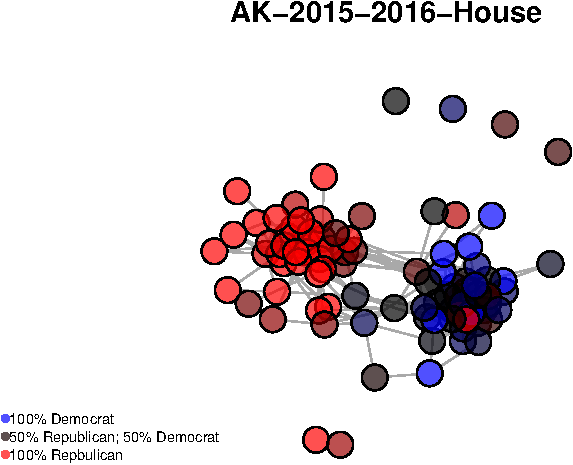
\includegraphics{Final_Project_RMarkdown_Updated_files/figure-latex/unnamed-chunk-10-1.pdf}
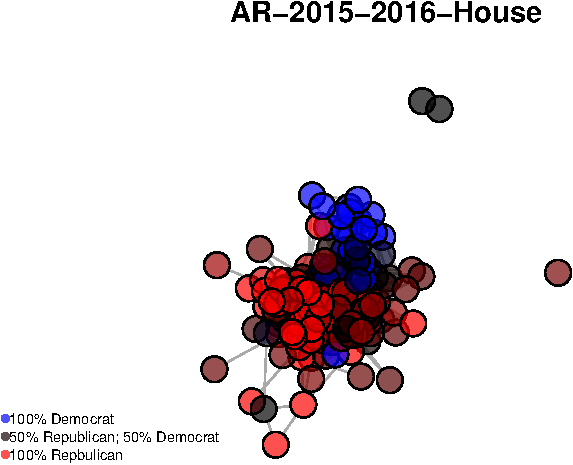
\includegraphics{Final_Project_RMarkdown_Updated_files/figure-latex/unnamed-chunk-10-2.pdf}
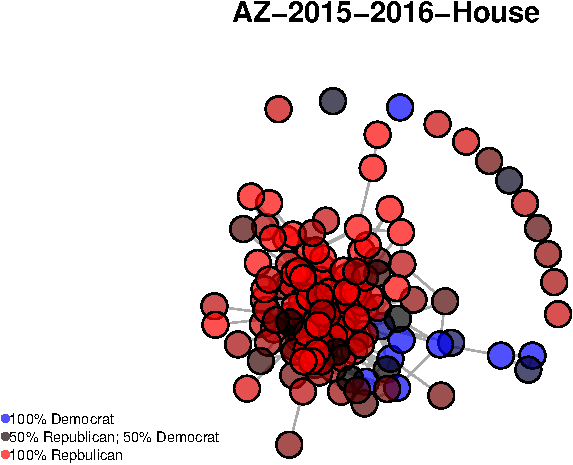
\includegraphics{Final_Project_RMarkdown_Updated_files/figure-latex/unnamed-chunk-10-3.pdf}
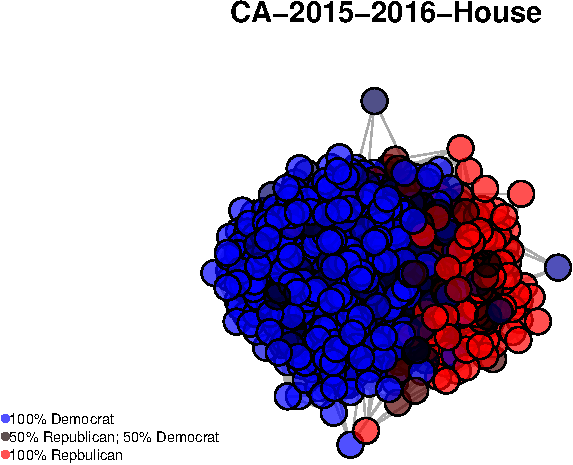
\includegraphics{Final_Project_RMarkdown_Updated_files/figure-latex/unnamed-chunk-10-4.pdf}
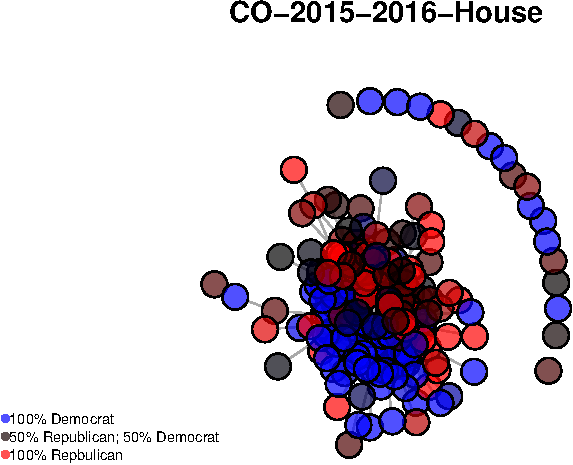
\includegraphics{Final_Project_RMarkdown_Updated_files/figure-latex/unnamed-chunk-10-5.pdf}
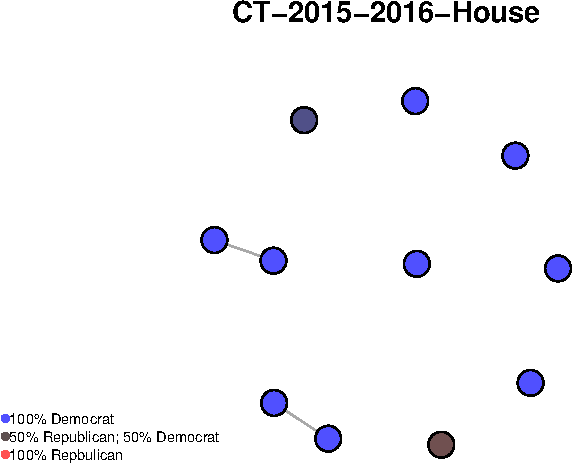
\includegraphics{Final_Project_RMarkdown_Updated_files/figure-latex/unnamed-chunk-10-6.pdf}
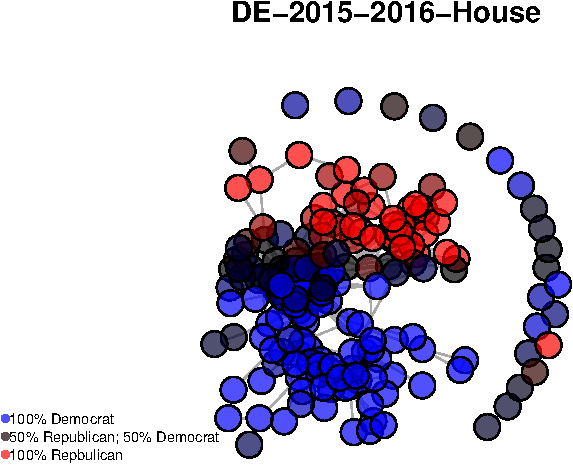
\includegraphics{Final_Project_RMarkdown_Updated_files/figure-latex/unnamed-chunk-10-7.pdf}
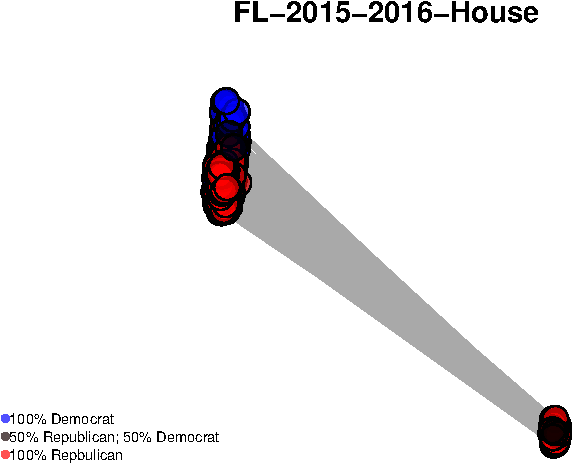
\includegraphics{Final_Project_RMarkdown_Updated_files/figure-latex/unnamed-chunk-10-8.pdf}
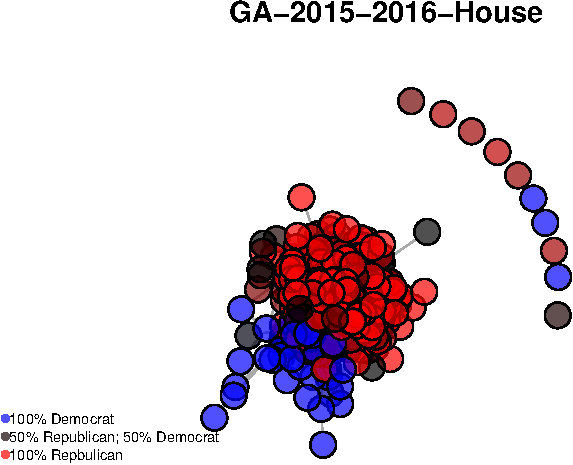
\includegraphics{Final_Project_RMarkdown_Updated_files/figure-latex/unnamed-chunk-10-9.pdf}
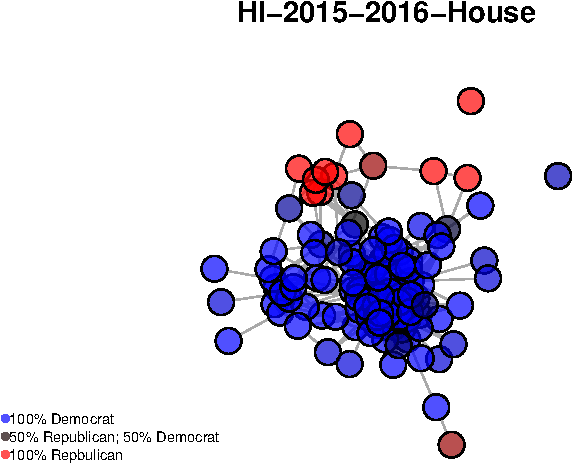
\includegraphics{Final_Project_RMarkdown_Updated_files/figure-latex/unnamed-chunk-10-10.pdf}
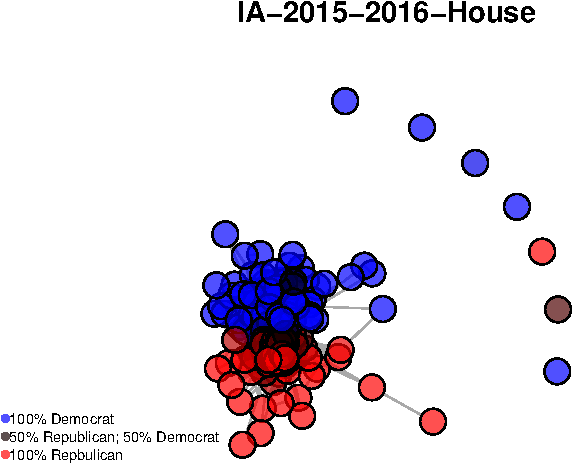
\includegraphics{Final_Project_RMarkdown_Updated_files/figure-latex/unnamed-chunk-10-11.pdf}
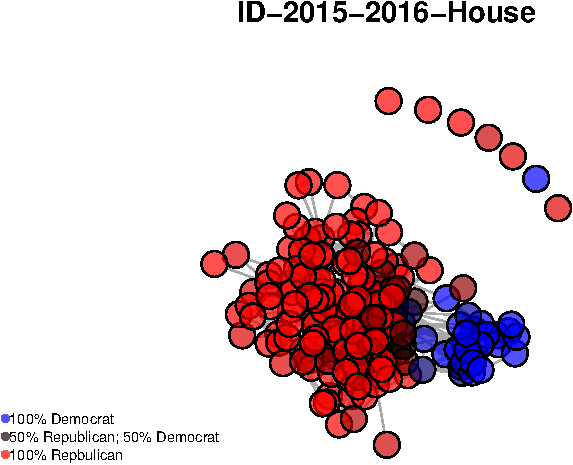
\includegraphics{Final_Project_RMarkdown_Updated_files/figure-latex/unnamed-chunk-10-12.pdf}
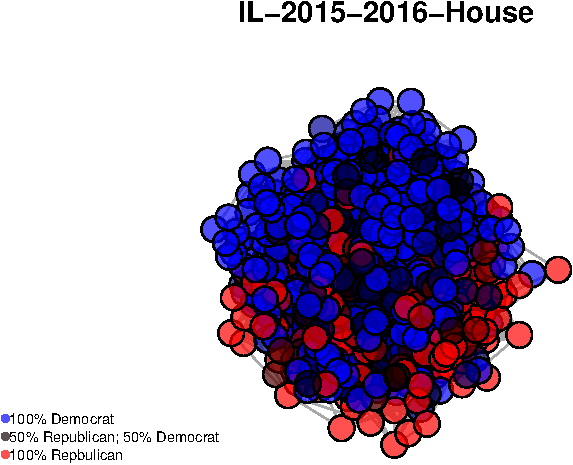
\includegraphics{Final_Project_RMarkdown_Updated_files/figure-latex/unnamed-chunk-10-13.pdf}
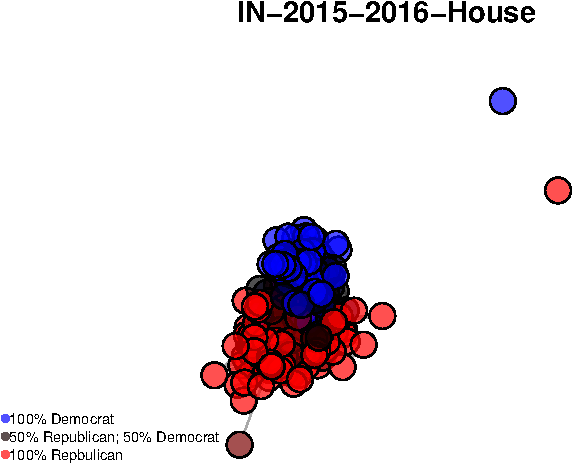
\includegraphics{Final_Project_RMarkdown_Updated_files/figure-latex/unnamed-chunk-10-14.pdf}
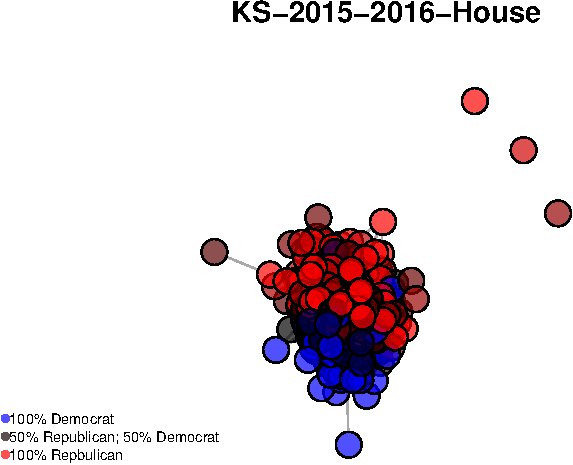
\includegraphics{Final_Project_RMarkdown_Updated_files/figure-latex/unnamed-chunk-10-15.pdf}
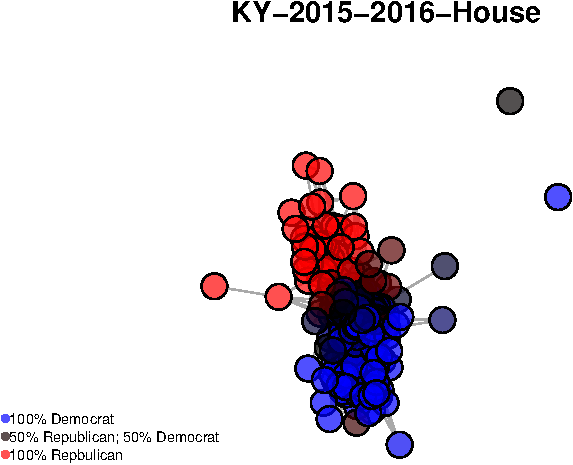
\includegraphics{Final_Project_RMarkdown_Updated_files/figure-latex/unnamed-chunk-10-16.pdf}
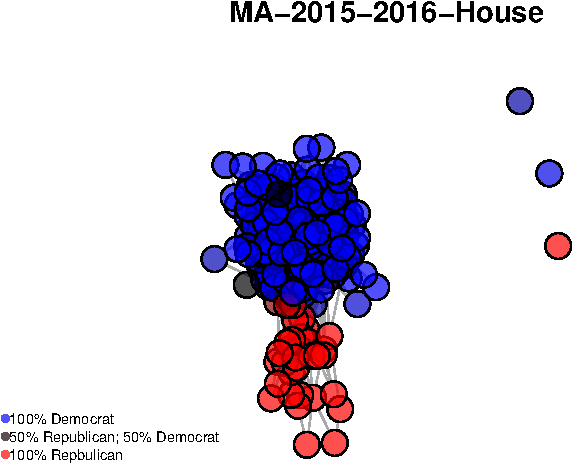
\includegraphics{Final_Project_RMarkdown_Updated_files/figure-latex/unnamed-chunk-10-17.pdf}
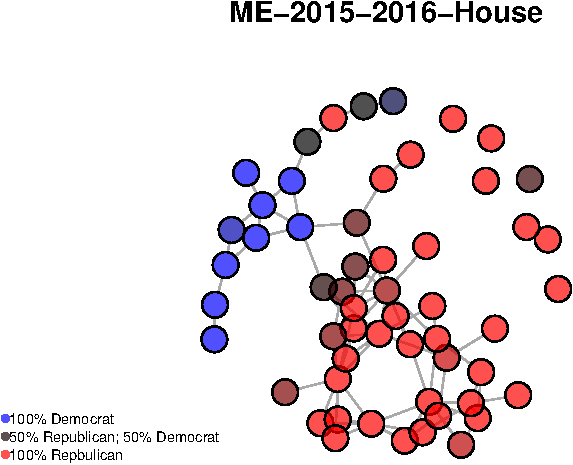
\includegraphics{Final_Project_RMarkdown_Updated_files/figure-latex/unnamed-chunk-10-18.pdf}
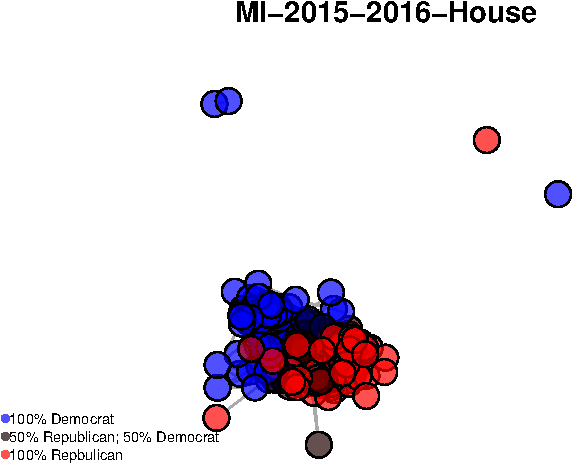
\includegraphics{Final_Project_RMarkdown_Updated_files/figure-latex/unnamed-chunk-10-19.pdf}
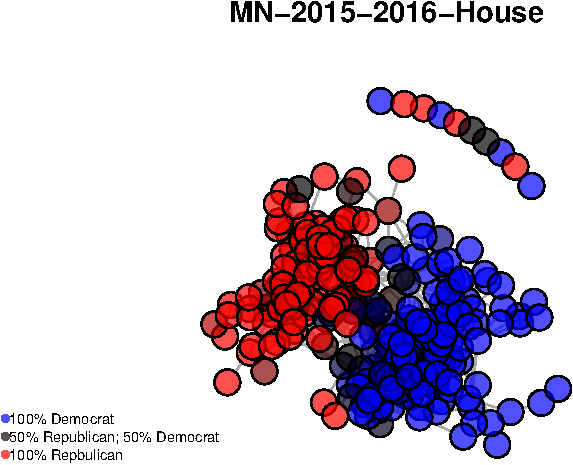
\includegraphics{Final_Project_RMarkdown_Updated_files/figure-latex/unnamed-chunk-10-20.pdf}
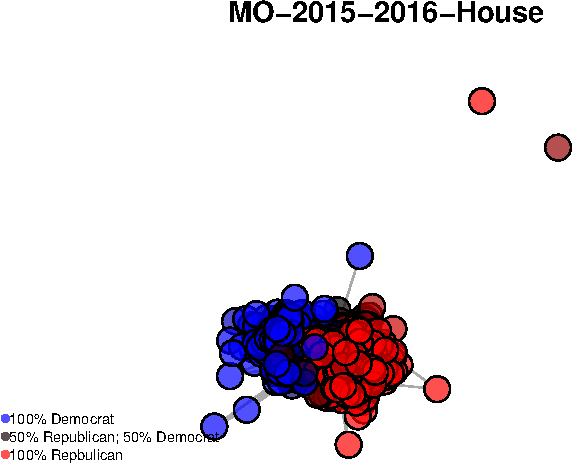
\includegraphics{Final_Project_RMarkdown_Updated_files/figure-latex/unnamed-chunk-10-21.pdf}
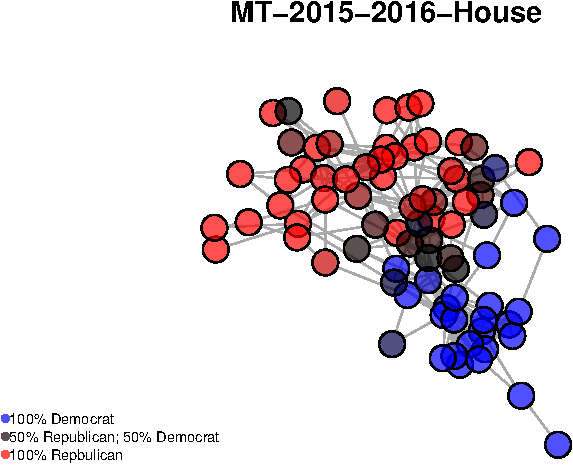
\includegraphics{Final_Project_RMarkdown_Updated_files/figure-latex/unnamed-chunk-10-22.pdf}
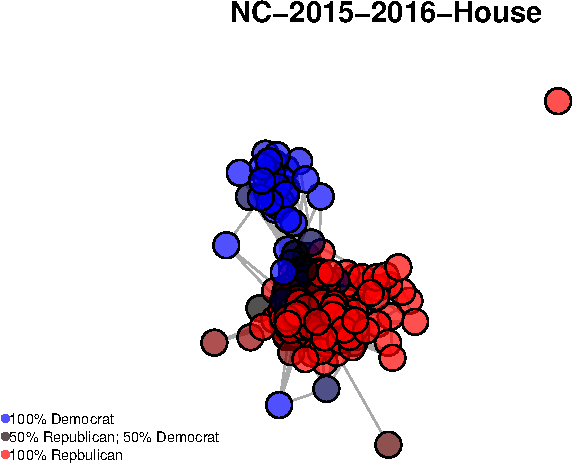
\includegraphics{Final_Project_RMarkdown_Updated_files/figure-latex/unnamed-chunk-10-23.pdf}
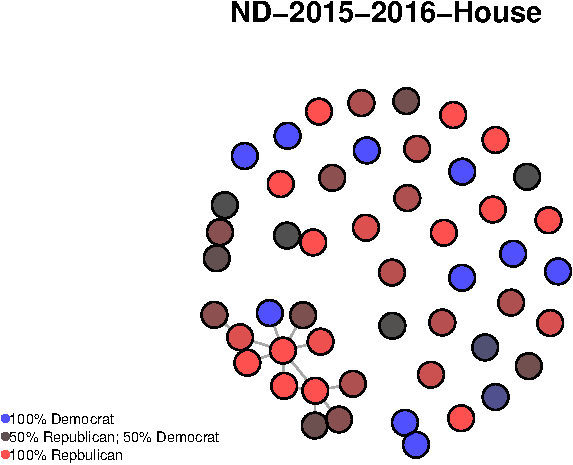
\includegraphics{Final_Project_RMarkdown_Updated_files/figure-latex/unnamed-chunk-10-24.pdf}
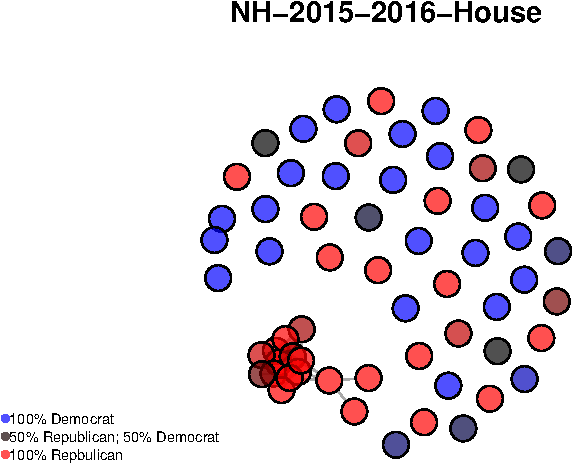
\includegraphics{Final_Project_RMarkdown_Updated_files/figure-latex/unnamed-chunk-10-25.pdf}
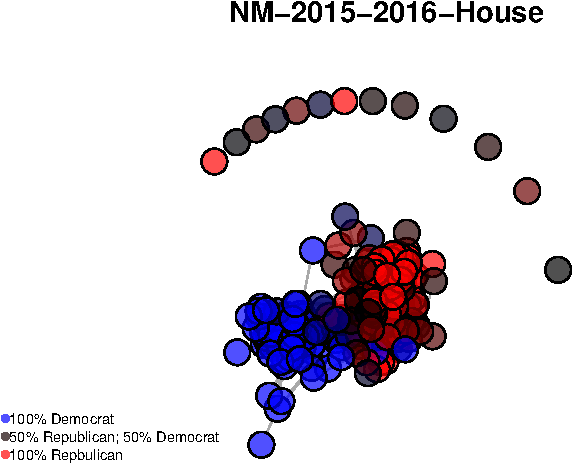
\includegraphics{Final_Project_RMarkdown_Updated_files/figure-latex/unnamed-chunk-10-26.pdf}
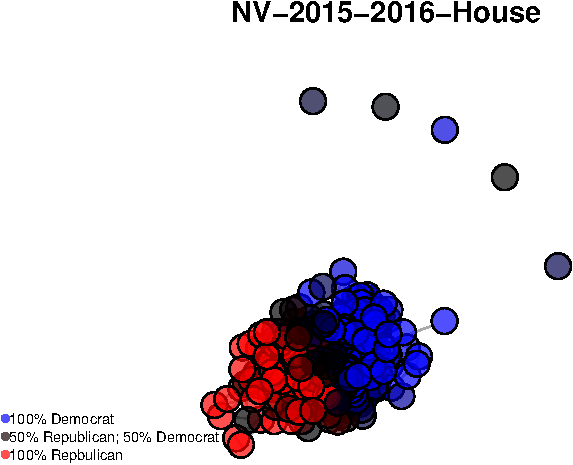
\includegraphics{Final_Project_RMarkdown_Updated_files/figure-latex/unnamed-chunk-10-27.pdf}
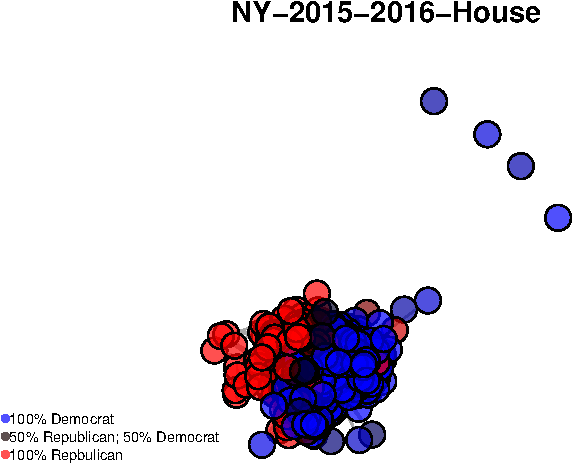
\includegraphics{Final_Project_RMarkdown_Updated_files/figure-latex/unnamed-chunk-10-28.pdf}
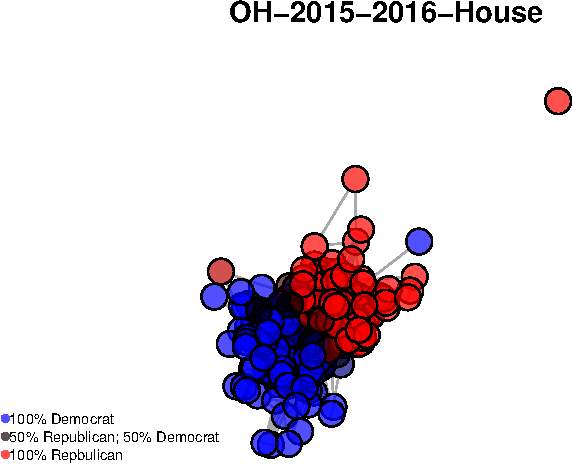
\includegraphics{Final_Project_RMarkdown_Updated_files/figure-latex/unnamed-chunk-10-29.pdf}
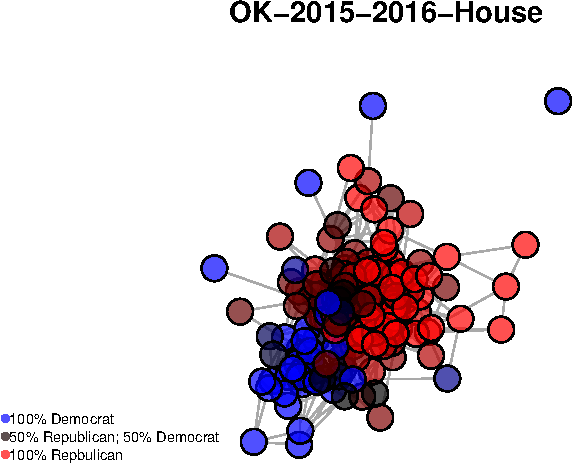
\includegraphics{Final_Project_RMarkdown_Updated_files/figure-latex/unnamed-chunk-10-30.pdf}
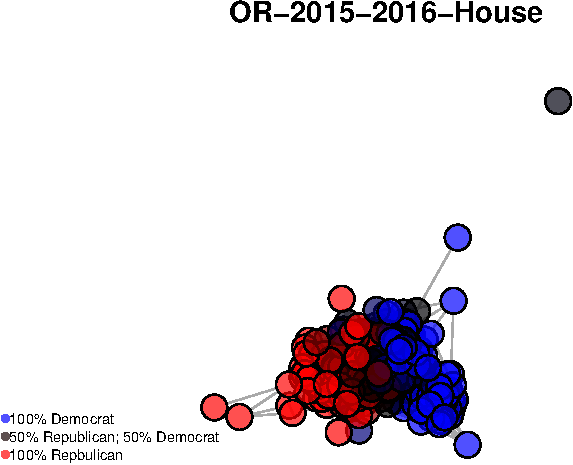
\includegraphics{Final_Project_RMarkdown_Updated_files/figure-latex/unnamed-chunk-10-31.pdf}
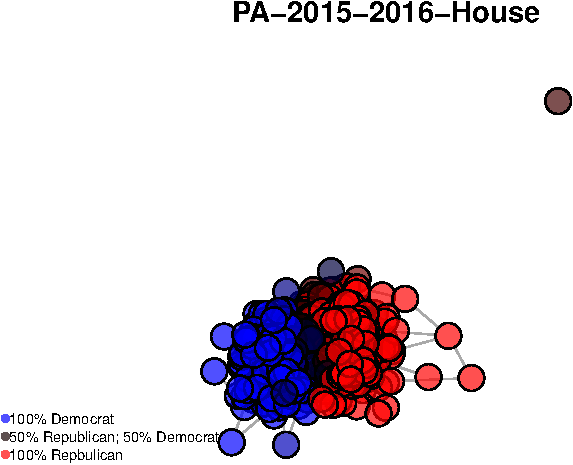
\includegraphics{Final_Project_RMarkdown_Updated_files/figure-latex/unnamed-chunk-10-32.pdf}
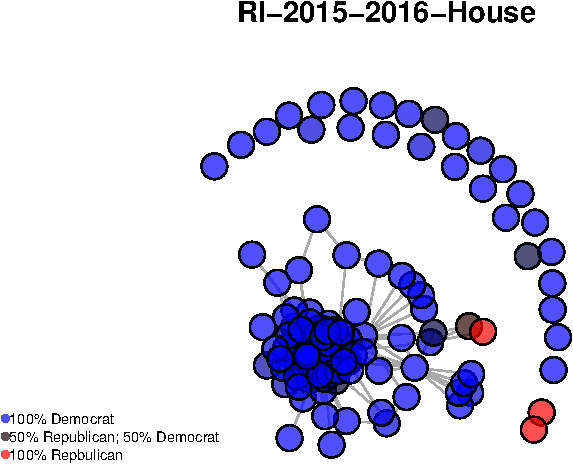
\includegraphics{Final_Project_RMarkdown_Updated_files/figure-latex/unnamed-chunk-10-33.pdf}
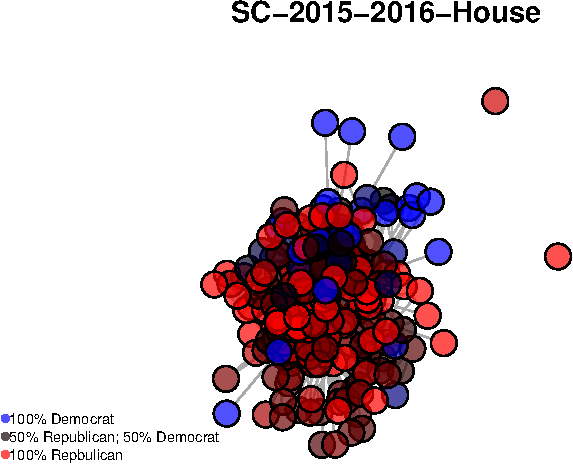
\includegraphics{Final_Project_RMarkdown_Updated_files/figure-latex/unnamed-chunk-10-34.pdf}
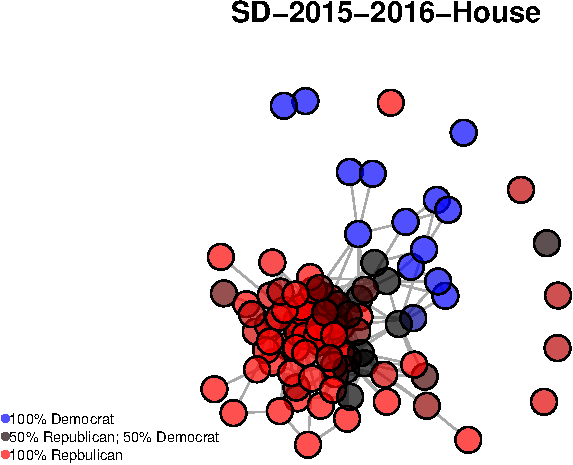
\includegraphics{Final_Project_RMarkdown_Updated_files/figure-latex/unnamed-chunk-10-35.pdf}
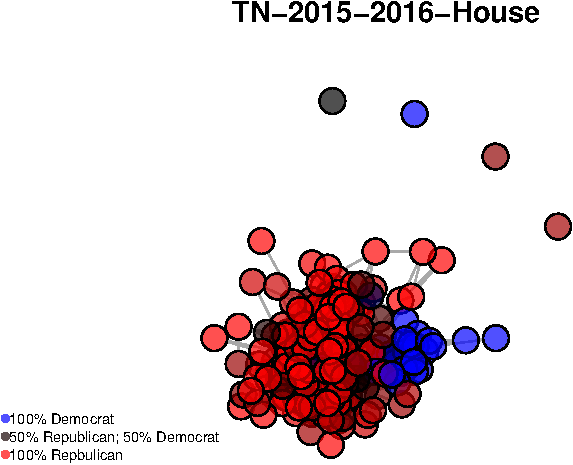
\includegraphics{Final_Project_RMarkdown_Updated_files/figure-latex/unnamed-chunk-10-36.pdf}
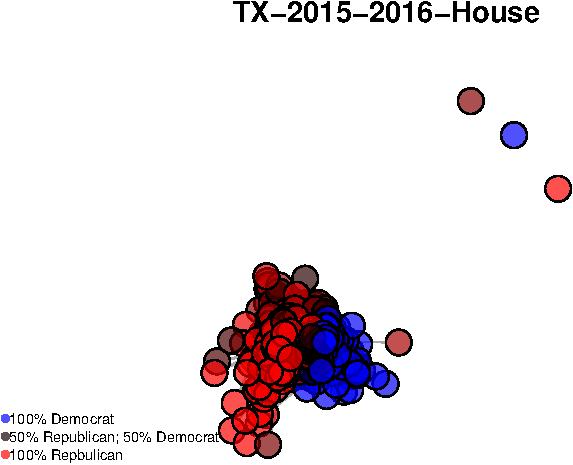
\includegraphics{Final_Project_RMarkdown_Updated_files/figure-latex/unnamed-chunk-10-37.pdf}
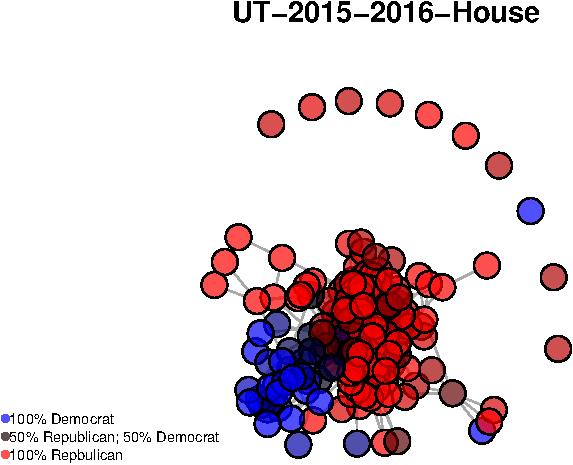
\includegraphics{Final_Project_RMarkdown_Updated_files/figure-latex/unnamed-chunk-10-38.pdf}
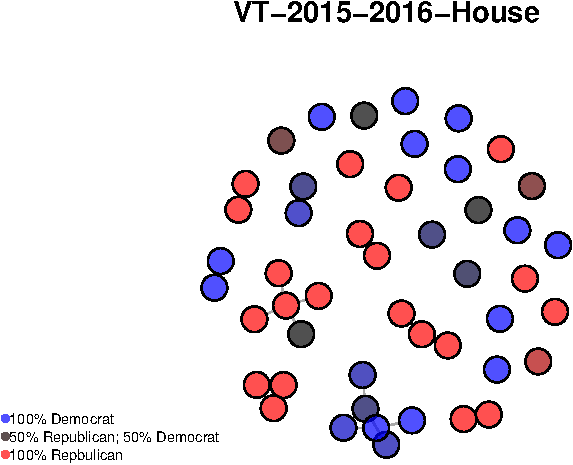
\includegraphics{Final_Project_RMarkdown_Updated_files/figure-latex/unnamed-chunk-10-39.pdf}
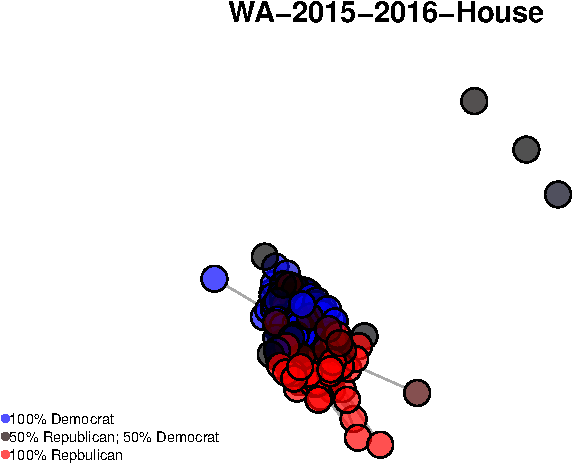
\includegraphics{Final_Project_RMarkdown_Updated_files/figure-latex/unnamed-chunk-10-40.pdf}
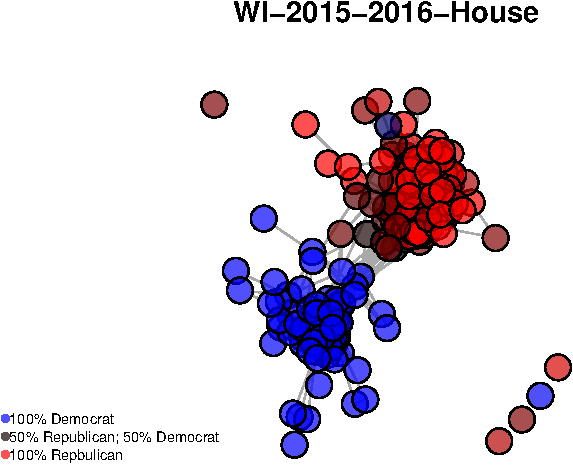
\includegraphics{Final_Project_RMarkdown_Updated_files/figure-latex/unnamed-chunk-10-41.pdf}
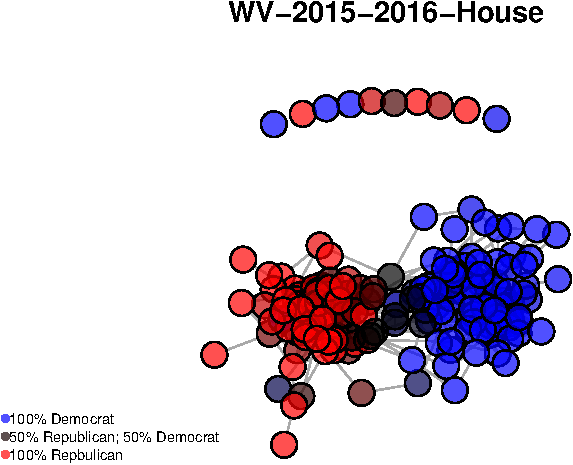
\includegraphics{Final_Project_RMarkdown_Updated_files/figure-latex/unnamed-chunk-10-42.pdf}
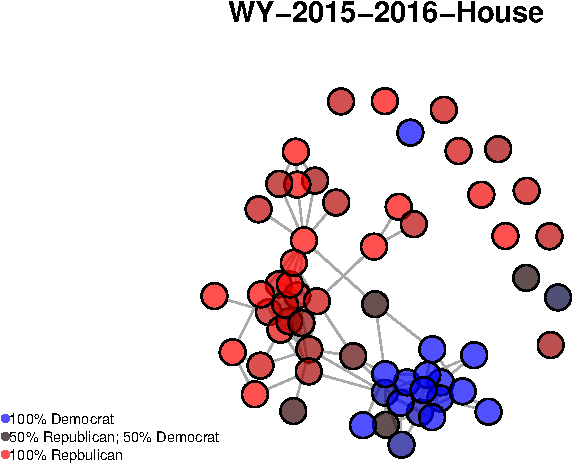
\includegraphics{Final_Project_RMarkdown_Updated_files/figure-latex/unnamed-chunk-10-43.pdf}
{[},1{]} {[},2{]} {[},3{]} {[},4{]} {[},5{]} {[},6{]} {[},7{]} {[},8{]}
{[},9{]} {[},10{]} rect List,4 List,4 List,4 List,4 List,4 List,4 List,4
List,4 List,4 List,4 text List,2 List,2 List,2 List,2 List,2 List,2
List,2 List,2 List,2 List,2 {[},11{]} {[},12{]} {[},13{]} {[},14{]}
{[},15{]} {[},16{]} {[},17{]} {[},18{]} {[},19{]} {[},20{]} rect List,4
List,4 List,4 List,4 List,4 List,4 List,4 List,4 List,4 List,4 text
List,2 List,2 List,2 List,2 List,2 List,2 List,2 List,2 List,2 List,2
{[},21{]} {[},22{]} {[},23{]} {[},24{]} {[},25{]} {[},26{]} {[},27{]}
{[},28{]} {[},29{]} {[},30{]} rect List,4 List,4 List,4 List,4 List,4
List,4 List,4 List,4 List,4 List,4 text List,2 List,2 List,2 List,2
List,2 List,2 List,2 List,2 List,2 List,2 {[},31{]} {[},32{]} {[},33{]}
{[},34{]} {[},35{]} {[},36{]} {[},37{]} {[},38{]} {[},39{]} {[},40{]}
rect List,4 List,4 List,4 List,4 List,4 List,4 List,4 List,4 List,4
List,4 text List,2 List,2 List,2 List,2 List,2 List,2 List,2 List,2
List,2 List,2 {[},41{]} {[},42{]} {[},43{]} rect List,4 List,4 List,4
text List,2 List,2 List,2

\begin{Shaded}
\begin{Highlighting}[]
\NormalTok{label <-}\StringTok{ }\KeywordTok{substr}\NormalTok{(y,}\DecValTok{1}\NormalTok{,}\DecValTok{2}\NormalTok{)}
\NormalTok{table <-}\StringTok{ }\KeywordTok{data.frame}\NormalTok{(label,}\DataTypeTok{density=}\KeywordTok{round}\NormalTok{(}\KeywordTok{unlist}\NormalTok{(density), }\DecValTok{3}\NormalTok{), }\DataTypeTok{diameter=}\KeywordTok{round}\NormalTok{(}\KeywordTok{unlist}\NormalTok{(diameter),}\DecValTok{3}\NormalTok{), }\DataTypeTok{mean_dist=}\KeywordTok{round}\NormalTok{(}\KeywordTok{unlist}\NormalTok{(mean_dist),}\DecValTok{3}\NormalTok{), }\DataTypeTok{cd=}\KeywordTok{round}\NormalTok{(}\KeywordTok{unlist}\NormalTok{(cd),}\DecValTok{3}\NormalTok{),}\DataTypeTok{cb=}\KeywordTok{round}\NormalTok{(}\KeywordTok{unlist}\NormalTok{(cb),}\DecValTok{3}\NormalTok{),}\DataTypeTok{ce=}\KeywordTok{round}\NormalTok{(}\KeywordTok{unlist}\NormalTok{(ce),}\DecValTok{3}\NormalTok{))}
\NormalTok{col_names <-}\StringTok{ }\KeywordTok{c}\NormalTok{(}\StringTok{"State"}\NormalTok{,}\StringTok{"Density"}\NormalTok{,}\StringTok{"Diameter"}\NormalTok{,}\StringTok{"Mean}\CharTok{\textbackslash{}n}\StringTok{Distance"}\NormalTok{,}\StringTok{"Degree}\CharTok{\textbackslash{}n}\StringTok{Centrality"}\NormalTok{,}\StringTok{"Betweeness}\CharTok{\textbackslash{}n}\StringTok{Centrality"}\NormalTok{,}\StringTok{"Eigenvector}\CharTok{\textbackslash{}n}\StringTok{Centrality"}\NormalTok{)}
\end{Highlighting}
\end{Shaded}

Below is a table showing the values for different centrality measures
for each state for the 2016 election:

\begin{Shaded}
\begin{Highlighting}[]
\NormalTok{table }\OperatorTok
\KeywordTok{mutate_all}\NormalTok{(linebreak) }\OperatorTok
\KeywordTok{kable}\NormalTok{(}\DataTypeTok{format=}\StringTok{"latex"}\NormalTok{,}\DataTypeTok{escape=}\NormalTok{F,}\DataTypeTok{row.names=}\OtherTok{FALSE}\NormalTok{,}\DataTypeTok{col.names=}\KeywordTok{linebreak}\NormalTok{(col_names), }\DataTypeTok{caption=}\StringTok{"Network Level Summary Statistics }\CharTok{\textbackslash{}n}\StringTok{ Election Year 2016"}\NormalTok{)}\OperatorTok
\KeywordTok{kable_styling}\NormalTok{(}\DataTypeTok{latex_options =} \KeywordTok{c}\NormalTok{(}\StringTok{"striped"}\NormalTok{, }\StringTok{"hold_position"}\NormalTok{))}
\end{Highlighting}
\end{Shaded}

\begin{table}[!h]

\caption{\label{tab:unnamed-chunk-12}Network Level Summary Statistics 
 Election Year 2016}
\centering
\begin{tabular}{l|r|r|r|r|r|r}
\hline
State & Density & Diameter & \makecell[l]{Mean\\Distance} & \makecell[l]{Degree\\Centrality} & \makecell[l]{Betweeness\\Centrality} & \makecell[l]{Eigenvector\\Centrality}\\
\hline
\rowcolor{gray!6}  AK & 0.118 & 6 & 2.563 & 0.145 & 0.182 & 0.740\\
\hline
AR & 0.110 & 5 & 2.298 & 0.200 & 0.035 & 0.753\\
\hline
\rowcolor{gray!6}  AZ & 0.078 & 7 & 2.612 & 0.354 & 0.150 & 0.819\\
\hline
CA & 0.229 & 4 & 1.782 & 0.285 & 0.002 & 0.584\\
\hline
\rowcolor{gray!6}  CO & 0.040 & 8 & 2.913 & 0.129 & 0.060 & 0.865\\
\hline
CT & 0.036 & 1 & 1.000 & 0.064 & 0.000 & 1.000\\
\hline
\rowcolor{gray!6}  DE & 0.056 & 8 & 3.086 & 0.222 & 0.110 & 0.831\\
\hline
FL & 0.173 & 4 & 1.860 & 0.377 & 0.006 & 0.659\\
\hline
\rowcolor{gray!6}  GA & 0.081 & 8 & 2.504 & 0.296 & 0.038 & 0.788\\
\hline
HI & 0.117 & 7 & 2.518 & 0.272 & 0.105 & 0.743\\
\hline
\rowcolor{gray!6}  IA & 0.365 & 5 & 1.723 & 0.310 & 0.025 & 0.447\\
\hline
ID & 0.073 & 6 & 2.769 & 0.185 & 0.087 & 0.797\\
\hline
\rowcolor{gray!6}  IL & 0.249 & 4 & 1.765 & 0.348 & 0.004 & 0.589\\
\hline
IN & 0.187 & 4 & 1.946 & 0.310 & 0.031 & 0.651\\
\hline
\rowcolor{gray!6}  KS & 0.078 & 5 & 2.317 & 0.200 & 0.025 & 0.797\\
\hline
KY & 0.171 & 5 & 2.059 & 0.218 & 0.034 & 0.654\\
\hline
\rowcolor{gray!6}  MA & 0.081 & 6 & 2.349 & 0.169 & 0.023 & 0.775\\
\hline
ME & 0.063 & 11 & 4.021 & 0.140 & 0.262 & 0.794\\
\hline
\rowcolor{gray!6}  MI & 0.160 & 4 & 1.965 & 0.253 & 0.015 & 0.685\\
\hline
MN & 0.031 & 10 & 3.591 & 0.075 & 0.064 & 0.901\\
\hline
\rowcolor{gray!6}  MO & 0.110 & 5 & 2.126 & 0.225 & 0.012 & 0.755\\
\hline
MT & 0.082 & 7 & 2.927 & 0.184 & 0.212 & 0.788\\
\hline
\rowcolor{gray!6}  NC & 0.305 & 5 & 1.857 & 0.320 & 0.021 & 0.528\\
\hline
ND & 0.015 & 4 & 2.113 & 0.128 & 0.035 & 0.931\\
\hline
\rowcolor{gray!6}  NH & 0.033 & 3 & 1.575 & 0.167 & 0.014 & 0.853\\
\hline
NM & 0.112 & 6 & 2.500 & 0.260 & 0.062 & 0.759\\
\hline
\rowcolor{gray!6}  NV & 0.108 & 5 & 2.263 & 0.280 & 0.022 & 0.765\\
\hline
NY & 0.109 & 5 & 2.166 & 0.248 & 0.014 & 0.744\\
\hline
\rowcolor{gray!6}  OH & 0.244 & 5 & 1.879 & 0.305 & 0.012 & 0.575\\
\hline
OK & 0.139 & 6 & 2.222 & 0.253 & 0.031 & 0.708\\
\hline
\rowcolor{gray!6}  OR & 0.172 & 5 & 2.006 & 0.319 & 0.023 & 0.687\\
\hline
PA & 0.100 & 5 & 2.157 & 0.241 & 0.011 & 0.761\\
\hline
\rowcolor{gray!6}  RI & 0.137 & 5 & 2.107 & 0.438 & 0.085 & 0.700\\
\hline
SC & 0.068 & 6 & 2.583 & 0.218 & 0.116 & 0.817\\
\hline
\rowcolor{gray!6}  SD & 0.123 & 6 & 2.388 & 0.265 & 0.058 & 0.713\\
\hline
TN & 0.112 & 6 & 2.292 & 0.260 & 0.040 & 0.739\\
\hline
\rowcolor{gray!6}  TX & 0.124 & 5 & 2.034 & 0.272 & 0.007 & 0.719\\
\hline
UT & 0.100 & 6 & 2.536 & 0.302 & 0.039 & 0.755\\
\hline
\rowcolor{gray!6}  VT & 0.019 & 3 & 1.444 & 0.066 & 0.005 & 0.953\\
\hline
WA & 0.212 & 4 & 1.854 & 0.274 & 0.006 & 0.620\\
\hline
\rowcolor{gray!6}  WI & 0.112 & 7 & 2.715 & 0.165 & 0.144 & 0.812\\
\hline
WV & 0.099 & 7 & 2.770 & 0.237 & 0.051 & 0.772\\
\hline
\rowcolor{gray!6}  WY & 0.086 & 6 & 2.936 & 0.134 & 0.152 & 0.795\\
\hline
\end{tabular}
\end{table}

\begin{Shaded}
\begin{Highlighting}[]
\NormalTok{tablesub <-}\StringTok{ }\NormalTok{table[table}\OperatorTok{$}\NormalTok{label}\OperatorTok{==}\StringTok{"MN"} \OperatorTok{|}\StringTok{ }\NormalTok{table}\OperatorTok{$}\NormalTok{label}\OperatorTok{==}\StringTok{"IA"} \OperatorTok{|}\StringTok{ }\NormalTok{table}\OperatorTok{$}\NormalTok{label}\OperatorTok{==}\StringTok{"WI"} \OperatorTok{|}\NormalTok{table}\OperatorTok{$}\NormalTok{label }\OperatorTok{==}\StringTok{"OH"} \OperatorTok{|}\StringTok{ }\NormalTok{table}\OperatorTok{$}\NormalTok{label}\OperatorTok{==}\StringTok{"ND"} \OperatorTok{|}\StringTok{ }\NormalTok{table}\OperatorTok{$}\NormalTok{label}\OperatorTok{==}\StringTok{"SD"} \OperatorTok{|}\StringTok{ }\NormalTok{table}\OperatorTok{$}\NormalTok{label}\OperatorTok{==}\StringTok{"MI"} \OperatorTok{|}\StringTok{ }\NormalTok{table}\OperatorTok{$}\NormalTok{label}\OperatorTok{==}\StringTok{"ID"} \OperatorTok{|}\NormalTok{table}\OperatorTok{$}\NormalTok{label}\OperatorTok{==}\StringTok{"IL"}\NormalTok{,]}
\KeywordTok{ggplot}\NormalTok{(tablesub)}\OperatorTok{+}
\StringTok{  }\KeywordTok{geom_point}\NormalTok{(}\KeywordTok{aes}\NormalTok{(label, }\KeywordTok{as.numeric}\NormalTok{(density), }\DataTypeTok{color=}\StringTok{"purple"}\NormalTok{))}\OperatorTok{+}
\StringTok{  }\KeywordTok{geom_point}\NormalTok{(}\KeywordTok{aes}\NormalTok{(label, }\KeywordTok{as.numeric}\NormalTok{(cd), }\DataTypeTok{color=}\StringTok{"red"}\NormalTok{))}\OperatorTok{+}
\StringTok{  }\KeywordTok{geom_point}\NormalTok{(}\KeywordTok{aes}\NormalTok{(label, }\KeywordTok{as.numeric}\NormalTok{(cb), }\DataTypeTok{color=}\StringTok{"blue"}\NormalTok{))}\OperatorTok{+}
\StringTok{  }\KeywordTok{geom_point}\NormalTok{(}\KeywordTok{aes}\NormalTok{(label, }\KeywordTok{as.numeric}\NormalTok{(ce), }\DataTypeTok{color=}\StringTok{"green"}\NormalTok{))}\OperatorTok{+}
\StringTok{  }\KeywordTok{labs}\NormalTok{(}\DataTypeTok{title=}\StringTok{"Network Centrality Measures}\CharTok{\textbackslash{}n}\StringTok{Electoral Years for Upper Midwest"}\NormalTok{, }\DataTypeTok{x=}\StringTok{"Electoral Year"}\NormalTok{, }\DataTypeTok{y=}\StringTok{"Centrality Measure"}\NormalTok{, }\DataTypeTok{color=}\StringTok{"Legend"}\NormalTok{)}\OperatorTok{+}
\StringTok{  }\KeywordTok{scale_color_manual}\NormalTok{(}\DataTypeTok{labels =}\KeywordTok{c}\NormalTok{(}\StringTok{"Density"}\NormalTok{,}\StringTok{"Degree Centrality"}\NormalTok{,}\StringTok{"Degree Betweeness"}\NormalTok{,}\StringTok{"Degree Eigenvector"}\NormalTok{), }\DataTypeTok{values=}\KeywordTok{c}\NormalTok{(}\StringTok{"purple"}\NormalTok{,}\StringTok{"red"}\NormalTok{,}\StringTok{"blue"}\NormalTok{,}\StringTok{"green"}\NormalTok{))}
\end{Highlighting}
\end{Shaded}

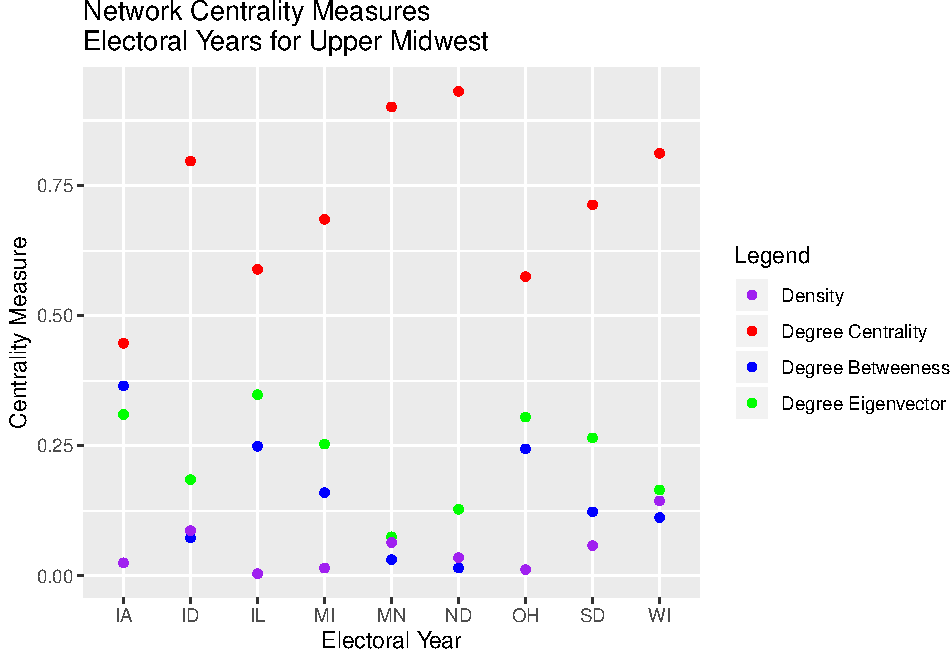
\includegraphics{Final_Project_RMarkdown_Updated_files/figure-latex/unnamed-chunk-13-1.pdf}

Degree centrality is consistently higher than the other centrality
measures in each state. Interestingly, there is no clear indication that
a particular state has a higher network level centrality. For instance,
North Dakota has the highest degree centrality but has the lowest degree
betweeness. This means that there is one or a few donor groups that have
many connections, but there aren't many donor groups that act as a
bridge to other donor groups. Looking at the plot of North Dakota in
2016 on the previous page, this makes a lot of sense. There appears to
be one or two donor groups that are connected to other donor groups and
a lot of isolate donor groups. In contrast, South Dakota's centrality
measures are closer together and this makes sense when looking at the
plot for South Dakota. It is clear that there are two clusters of donor
groups-one Republican and one Democrat-but there appear to be many donor
groups that are connected to others and far fewer isolates than in North
Dakota.

\subsection{First Set}\label{first-set-1}

\subsection{Scenario 1}\label{scenario-1}

\subsubsection{Same number of Republican and Democratic candidates as
reality}\label{same-number-of-republican-and-democratic-candidates-as-reality}

\begin{Shaded}
\begin{Highlighting}[]
\NormalTok{##I create a vector that captures the unique ID for state and year}
\NormalTok{y <-}\StringTok{ }\NormalTok{x[}\KeywordTok{str_detect}\NormalTok{(x,}\StringTok{"House"}\NormalTok{,}\DataTypeTok{negate=}\OtherTok{FALSE}\NormalTok{)}\OperatorTok{==}\OtherTok{TRUE}\NormalTok{]}
\NormalTok{seq <-}\StringTok{ }\KeywordTok{seq}\NormalTok{(}\DecValTok{1}\NormalTok{,}\DataTypeTok{by=}\DecValTok{1}\NormalTok{, }\DataTypeTok{len=}\KeywordTok{length}\NormalTok{(y))}

\NormalTok{##Create a variables}
\NormalTok{s <-}\StringTok{ }\KeywordTok{list}\NormalTok{()}
\NormalTok{m <-}\StringTok{ }\KeywordTok{list}\NormalTok{()}
\NormalTok{cd <-}\StringTok{ }\KeywordTok{vector}\NormalTok{()}
\NormalTok{cb <-}\StringTok{ }\KeywordTok{vector}\NormalTok{()}
\NormalTok{ce <-}\StringTok{ }\KeywordTok{vector}\NormalTok{()}
\NormalTok{d <-}\StringTok{ }\KeywordTok{vector}\NormalTok{()}
\NormalTok{n <-}\StringTok{ }\KeywordTok{list}\NormalTok{()}
\NormalTok{mean_cd1 <-}\StringTok{ }\KeywordTok{vector}\NormalTok{()}
\NormalTok{mean_cb1 <-}\StringTok{ }\KeywordTok{vector}\NormalTok{()}
\NormalTok{mean_ce1 <-}\StringTok{ }\KeywordTok{vector}\NormalTok{()}
\NormalTok{mean_d1 <-}\StringTok{ }\KeywordTok{vector}\NormalTok{()}
\NormalTok{l <-}\StringTok{ }\DecValTok{10}
\end{Highlighting}
\end{Shaded}

I first create a list with all of the datasets broken up by state and
election year.

\begin{Shaded}
\begin{Highlighting}[]
\NormalTok{md_subdata <-}\StringTok{ }\KeywordTok{lapply}\NormalTok{(seq, }\ControlFlowTok{function}\NormalTok{(k) md_house[}\KeywordTok{endsWith}\NormalTok{(md_house}\OperatorTok{$}\NormalTok{filename,y[k]),] )}
\NormalTok{full <-}\StringTok{ }\KeywordTok{lapply}\NormalTok{(}\DecValTok{1}\OperatorTok{:}\KeywordTok{length}\NormalTok{(md_subdata), }\ControlFlowTok{function}\NormalTok{(x) }\KeywordTok{merge}\NormalTok{(md_subdata[[x]], vote_cand, }\DataTypeTok{by=}\StringTok{"cat"}\NormalTok{))}
\NormalTok{n <-}\StringTok{ }\KeywordTok{lapply}\NormalTok{(}\DecValTok{1}\OperatorTok{:}\KeywordTok{length}\NormalTok{(full), }\ControlFlowTok{function}\NormalTok{(x) }\KeywordTok{nrow}\NormalTok{(full[[x]]))}
\end{Highlighting}
\end{Shaded}

Then I create vectors for the candidates that each donor had donated to
for each election in each state using the number of Democratic and
Republican candidates and the probability of a donor group donating to a
Democratic or Republican candidate.

\begin{Shaded}
\begin{Highlighting}[]
\NormalTok{s <-}\StringTok{ }\KeywordTok{replicate}\NormalTok{(l,}\KeywordTok{lapply}\NormalTok{(}\DecValTok{1}\OperatorTok{:}\KeywordTok{length}\NormalTok{(n), }\ControlFlowTok{function}\NormalTok{(x) }\KeywordTok{lapply}\NormalTok{(}\DecValTok{1}\OperatorTok{:}\NormalTok{n[[x]], }\ControlFlowTok{function}\NormalTok{(i) }\KeywordTok{c}\NormalTok{(}\KeywordTok{rbinom}\NormalTok{(full[[x]]}\OperatorTok{$}\NormalTok{num_dem[}\DecValTok{1}\NormalTok{], }\DecValTok{1}\NormalTok{,full[[x]]}\OperatorTok{$}\NormalTok{PerDem[i]}\OperatorTok{/}\DecValTok{100}\NormalTok{),}\KeywordTok{rbinom}\NormalTok{(full[[x]]}\OperatorTok{$}\NormalTok{num_rep[}\DecValTok{1}\NormalTok{],}\DecValTok{1}\NormalTok{,full[[x]]}\OperatorTok{$}\NormalTok{PerRep[i]}\OperatorTok{/}\DecValTok{100}\NormalTok{)))))}
\end{Highlighting}
\end{Shaded}

I create a function that will create a bipartite matrix and then an
incident matrix of donor groups.

\begin{Shaded}
\begin{Highlighting}[]
\NormalTok{matrix_graph_function <-}\StringTok{ }\ControlFlowTok{function}\NormalTok{(j,k,p)\{}
\NormalTok{  ##Below, I combine these vectors to create a bipartite network incidence matrix with the candidates as columns and the groups of donors as rows making it a GxC matrix.}

\NormalTok{  vec <-}\StringTok{ }\KeywordTok{unlist}\NormalTok{(j[k,p])}
\NormalTok{  m <-}\StringTok{ }\KeywordTok{matrix}\NormalTok{(vec,}\DataTypeTok{nrow=}\NormalTok{full[[k]]}\OperatorTok{$}\NormalTok{num_dem[}\DecValTok{1}\NormalTok{]}\OperatorTok{+}\NormalTok{full[[k]]}\OperatorTok{$}\NormalTok{num_rep[}\DecValTok{1}\NormalTok{], }\DataTypeTok{ncol=}\NormalTok{n[[k]])}
  
\NormalTok{##Now that I have the incidence matrix, I can convert the incidence matrix into a graph object and then project the bipartite graph to two one-mode networks. The second projection gives the GxG matrix, which is the one-mode network for groups of donors.}

\NormalTok{  g <-}\StringTok{ }\KeywordTok{graph_from_incidence_matrix}\NormalTok{(m)}
\NormalTok{  b <-}\StringTok{ }\KeywordTok{bipartite.projection}\NormalTok{(g)}\OperatorTok{$}\NormalTok{proj2}
  \KeywordTok{return}\NormalTok{(b)}
\NormalTok{\}}
\end{Highlighting}
\end{Shaded}

Now I have the function to create the donor group networks and all of
the simulated data, which is stored in s. I next create a list that
includes all of the one-mode graphs for all states and all simulations.

\begin{Shaded}
\begin{Highlighting}[]
\NormalTok{all_graphs <-}\StringTok{ }\KeywordTok{lapply}\NormalTok{(}\DecValTok{1}\OperatorTok{:}\KeywordTok{nrow}\NormalTok{(s), }\ControlFlowTok{function}\NormalTok{(t) }\KeywordTok{lapply}\NormalTok{(}\DecValTok{1}\OperatorTok{:}\KeywordTok{ncol}\NormalTok{(s), }\ControlFlowTok{function}\NormalTok{(x) }\KeywordTok{matrix_graph_function}\NormalTok{(s,t,x)))}
\end{Highlighting}
\end{Shaded}

Now I use those graphs to calculate network level centrality measures

\begin{Shaded}
\begin{Highlighting}[]
\NormalTok{##I now can calculate the centrality of the network.}
\NormalTok{  d <-}\StringTok{ }\KeywordTok{lapply}\NormalTok{(}\DecValTok{1}\OperatorTok{:}\KeywordTok{nrow}\NormalTok{(s), }\ControlFlowTok{function}\NormalTok{(t) }\KeywordTok{lapply}\NormalTok{(}\DecValTok{1}\OperatorTok{:}\KeywordTok{ncol}\NormalTok{(s), }\ControlFlowTok{function}\NormalTok{(x) }\KeywordTok{edge_density}\NormalTok{(all_graphs[[t]][[x]], }\DataTypeTok{loops=}\OtherTok{FALSE}\NormalTok{)))}
\NormalTok{  cd <-}\StringTok{ }\KeywordTok{lapply}\NormalTok{(}\DecValTok{1}\OperatorTok{:}\KeywordTok{nrow}\NormalTok{(s), }\ControlFlowTok{function}\NormalTok{(t) }\KeywordTok{lapply}\NormalTok{(}\DecValTok{1}\OperatorTok{:}\KeywordTok{ncol}\NormalTok{(s), }\ControlFlowTok{function}\NormalTok{(x) }\KeywordTok{centr_degree}\NormalTok{(all_graphs[[t]][[x]])}\OperatorTok{$}\NormalTok{centralization))}
  \CommentTok{#cb <- lapply(1:nrow(s), function(t) lapply(1:ncol(s), function(x) centr_betw(all_graphs[[t]][[x]])$centralization))}
\NormalTok{  ce <-}\StringTok{ }\KeywordTok{lapply}\NormalTok{(}\DecValTok{1}\OperatorTok{:}\KeywordTok{nrow}\NormalTok{(s), }\ControlFlowTok{function}\NormalTok{(t) }\KeywordTok{lapply}\NormalTok{(}\DecValTok{1}\OperatorTok{:}\KeywordTok{ncol}\NormalTok{(s), }\ControlFlowTok{function}\NormalTok{(x) }\KeywordTok{centr_eigen}\NormalTok{(all_graphs[[t]][[x]])}\OperatorTok{$}\NormalTok{centralization))}

\NormalTok{mean_cd1 <-}\StringTok{ }\KeywordTok{lapply}\NormalTok{(}\DecValTok{1}\OperatorTok{:}\KeywordTok{nrow}\NormalTok{(s), }\ControlFlowTok{function}\NormalTok{(x) }\KeywordTok{mean}\NormalTok{(}\KeywordTok{unlist}\NormalTok{(cd[[x]])))}
\CommentTok{#mean_cb1 <- lapply(1:nrow(s), function(x) mean(unlist(cb[[x]])))}
\NormalTok{mean_ce1 <-}\StringTok{ }\KeywordTok{lapply}\NormalTok{(}\DecValTok{1}\OperatorTok{:}\KeywordTok{nrow}\NormalTok{(s), }\ControlFlowTok{function}\NormalTok{(x) }\KeywordTok{mean}\NormalTok{(}\KeywordTok{unlist}\NormalTok{(ce[[x]])))}
\NormalTok{mean_d1 <-}\StringTok{ }\KeywordTok{lapply}\NormalTok{(}\DecValTok{1}\OperatorTok{:}\KeywordTok{nrow}\NormalTok{(s), }\ControlFlowTok{function}\NormalTok{(x) }\KeywordTok{mean}\NormalTok{(}\KeywordTok{unlist}\NormalTok{(d[[x]])))}
\end{Highlighting}
\end{Shaded}

\subsection{Scenario 2}\label{scenario-2}

\subsubsection{One more Republican candidate and same number of
Democratic candidates as
reality}\label{one-more-republican-candidate-and-same-number-of-democratic-candidates-as-reality}

I do not include the comments between each step to save space. The
methodology is exactly the same as in scenario one except for the number
of cnadiates changes.

\begin{Shaded}
\begin{Highlighting}[]
\NormalTok{##Create a variables}
\NormalTok{s <-}\StringTok{ }\KeywordTok{list}\NormalTok{()}
\NormalTok{m <-}\StringTok{ }\KeywordTok{list}\NormalTok{()}
\NormalTok{cd <-}\StringTok{ }\KeywordTok{vector}\NormalTok{()}
\NormalTok{cb <-}\StringTok{ }\KeywordTok{vector}\NormalTok{()}
\NormalTok{ce <-}\StringTok{ }\KeywordTok{vector}\NormalTok{()}
\NormalTok{d <-}\StringTok{ }\KeywordTok{vector}\NormalTok{()}
\NormalTok{n <-}\StringTok{ }\KeywordTok{list}\NormalTok{()}
\NormalTok{mean_cd2 <-}\StringTok{ }\KeywordTok{vector}\NormalTok{()}
\NormalTok{mean_cb2 <-}\StringTok{ }\KeywordTok{vector}\NormalTok{()}
\NormalTok{mean_ce2 <-}\StringTok{ }\KeywordTok{vector}\NormalTok{()}
\NormalTok{mean_d2 <-}\StringTok{ }\KeywordTok{vector}\NormalTok{()}
\NormalTok{l <-}\StringTok{ }\DecValTok{10}
\end{Highlighting}
\end{Shaded}

\begin{Shaded}
\begin{Highlighting}[]
\NormalTok{md_subdata <-}\StringTok{ }\KeywordTok{lapply}\NormalTok{(seq, }\ControlFlowTok{function}\NormalTok{(k) md_house[}\KeywordTok{endsWith}\NormalTok{(md_house}\OperatorTok{$}\NormalTok{filename,y[k]),] )}
\NormalTok{full <-}\StringTok{ }\KeywordTok{lapply}\NormalTok{(}\DecValTok{1}\OperatorTok{:}\KeywordTok{length}\NormalTok{(md_subdata), }\ControlFlowTok{function}\NormalTok{(x) }\KeywordTok{merge}\NormalTok{(md_subdata[[x]], vote_cand, }\DataTypeTok{by=}\StringTok{"cat"}\NormalTok{))}
\NormalTok{n <-}\StringTok{ }\KeywordTok{lapply}\NormalTok{(}\DecValTok{1}\OperatorTok{:}\KeywordTok{length}\NormalTok{(full), }\ControlFlowTok{function}\NormalTok{(x) }\KeywordTok{nrow}\NormalTok{(full[[x]]))}
\end{Highlighting}
\end{Shaded}

\begin{Shaded}
\begin{Highlighting}[]
\NormalTok{s <-}\StringTok{ }\KeywordTok{replicate}\NormalTok{(l,}\KeywordTok{lapply}\NormalTok{(}\DecValTok{1}\OperatorTok{:}\KeywordTok{length}\NormalTok{(n), }\ControlFlowTok{function}\NormalTok{(x) }\KeywordTok{lapply}\NormalTok{(}\DecValTok{1}\OperatorTok{:}\NormalTok{n[[x]], }\ControlFlowTok{function}\NormalTok{(i) }\KeywordTok{c}\NormalTok{(}\KeywordTok{rbinom}\NormalTok{(full[[x]]}\OperatorTok{$}\NormalTok{num_dem[}\DecValTok{1}\NormalTok{], }\DecValTok{1}\NormalTok{,full[[x]]}\OperatorTok{$}\NormalTok{PerDem[i]}\OperatorTok{/}\DecValTok{100}\NormalTok{),}\KeywordTok{rbinom}\NormalTok{(full[[x]]}\OperatorTok{$}\NormalTok{num_rep[}\DecValTok{1}\NormalTok{]}\OperatorTok{+}\DecValTok{1}\NormalTok{,}\DecValTok{1}\NormalTok{,full[[x]]}\OperatorTok{$}\NormalTok{PerRep[i]}\OperatorTok{/}\DecValTok{100}\NormalTok{)))))}
\end{Highlighting}
\end{Shaded}

\begin{Shaded}
\begin{Highlighting}[]
\NormalTok{matrix_graph_function <-}\StringTok{ }\ControlFlowTok{function}\NormalTok{(j,k,p)\{}
\NormalTok{  ##Below, I combine these vectors to create a bipartite network incidence matrix with the candidates as columns and the groups of donors as rows making it a GxC matrix.}

\NormalTok{  vec <-}\StringTok{ }\KeywordTok{unlist}\NormalTok{(j[k,p])}
\NormalTok{  m <-}\StringTok{ }\KeywordTok{matrix}\NormalTok{(vec,}\DataTypeTok{nrow=}\NormalTok{full[[k]]}\OperatorTok{$}\NormalTok{num_dem[}\DecValTok{1}\NormalTok{]}\OperatorTok{+}\NormalTok{full[[k]]}\OperatorTok{$}\NormalTok{num_rep[}\DecValTok{1}\NormalTok{]}\OperatorTok{+}\DecValTok{1}\NormalTok{, }\DataTypeTok{ncol=}\NormalTok{n[[k]])}
  

\NormalTok{  g <-}\StringTok{ }\KeywordTok{graph_from_incidence_matrix}\NormalTok{(m)}
\NormalTok{  b <-}\StringTok{ }\KeywordTok{bipartite.projection}\NormalTok{(g)}\OperatorTok{$}\NormalTok{proj2}
  \KeywordTok{return}\NormalTok{(b)}
\NormalTok{\}}
\end{Highlighting}
\end{Shaded}

\begin{Shaded}
\begin{Highlighting}[]
\NormalTok{all_graphs <-}\StringTok{ }\KeywordTok{lapply}\NormalTok{(}\DecValTok{1}\OperatorTok{:}\KeywordTok{nrow}\NormalTok{(s), }\ControlFlowTok{function}\NormalTok{(t) }\KeywordTok{lapply}\NormalTok{(}\DecValTok{1}\OperatorTok{:}\KeywordTok{ncol}\NormalTok{(s), }\ControlFlowTok{function}\NormalTok{(x) }\KeywordTok{matrix_graph_function}\NormalTok{(s,t,x)))}
\end{Highlighting}
\end{Shaded}

\begin{Shaded}
\begin{Highlighting}[]
\NormalTok{##I now can calculate the centrality of the network.}
\NormalTok{  d <-}\StringTok{ }\KeywordTok{lapply}\NormalTok{(}\DecValTok{1}\OperatorTok{:}\KeywordTok{nrow}\NormalTok{(s), }\ControlFlowTok{function}\NormalTok{(t) }\KeywordTok{lapply}\NormalTok{(}\DecValTok{1}\OperatorTok{:}\KeywordTok{ncol}\NormalTok{(s), }\ControlFlowTok{function}\NormalTok{(x) }\KeywordTok{edge_density}\NormalTok{(all_graphs[[t]][[x]], }\DataTypeTok{loops=}\OtherTok{FALSE}\NormalTok{)))}
\NormalTok{  cd <-}\StringTok{ }\KeywordTok{lapply}\NormalTok{(}\DecValTok{1}\OperatorTok{:}\KeywordTok{nrow}\NormalTok{(s), }\ControlFlowTok{function}\NormalTok{(t) }\KeywordTok{lapply}\NormalTok{(}\DecValTok{1}\OperatorTok{:}\KeywordTok{ncol}\NormalTok{(s), }\ControlFlowTok{function}\NormalTok{(x) }\KeywordTok{centr_degree}\NormalTok{(all_graphs[[t]][[x]])}\OperatorTok{$}\NormalTok{centralization))}
  \CommentTok{#cb <- lapply(1:nrow(s), function(t) lapply(1:ncol(s), function(x) centr_betw(all_graphs[[t]][[x]])$centralization))}
\NormalTok{  ce <-}\StringTok{ }\KeywordTok{lapply}\NormalTok{(}\DecValTok{1}\OperatorTok{:}\KeywordTok{nrow}\NormalTok{(s), }\ControlFlowTok{function}\NormalTok{(t) }\KeywordTok{lapply}\NormalTok{(}\DecValTok{1}\OperatorTok{:}\KeywordTok{ncol}\NormalTok{(s), }\ControlFlowTok{function}\NormalTok{(x) }\KeywordTok{centr_eigen}\NormalTok{(all_graphs[[t]][[x]])}\OperatorTok{$}\NormalTok{centralization))}

\NormalTok{mean_cd2 <-}\StringTok{ }\KeywordTok{lapply}\NormalTok{(}\DecValTok{1}\OperatorTok{:}\KeywordTok{nrow}\NormalTok{(s), }\ControlFlowTok{function}\NormalTok{(x) }\KeywordTok{mean}\NormalTok{(}\KeywordTok{unlist}\NormalTok{(cd[[x]])))}
\CommentTok{#mean_cb2 <- lapply(1:nrow(s), function(x) mean(unlist(cb[[x]])))}
\NormalTok{mean_ce2 <-}\StringTok{ }\KeywordTok{lapply}\NormalTok{(}\DecValTok{1}\OperatorTok{:}\KeywordTok{nrow}\NormalTok{(s), }\ControlFlowTok{function}\NormalTok{(x) }\KeywordTok{mean}\NormalTok{(}\KeywordTok{unlist}\NormalTok{(ce[[x]])))}
\NormalTok{mean_d2 <-}\StringTok{ }\KeywordTok{lapply}\NormalTok{(}\DecValTok{1}\OperatorTok{:}\KeywordTok{nrow}\NormalTok{(s), }\ControlFlowTok{function}\NormalTok{(x) }\KeywordTok{mean}\NormalTok{(}\KeywordTok{unlist}\NormalTok{(d[[x]])))}
\end{Highlighting}
\end{Shaded}

\subsection{Scenario 3}\label{scenario-3}

\subsubsection{One more Democratic candidate and same number of
Republican candidates as
reality}\label{one-more-democratic-candidate-and-same-number-of-republican-candidates-as-reality}

I do not include the comments between each step to save space. The
methodology is exactly the same as in scenario one except for the number
of cnadiates changes.

\begin{Shaded}
\begin{Highlighting}[]
\NormalTok{##Create a variables}
\NormalTok{s <-}\StringTok{ }\KeywordTok{list}\NormalTok{()}
\NormalTok{m <-}\StringTok{ }\KeywordTok{list}\NormalTok{()}
\NormalTok{cd <-}\StringTok{ }\KeywordTok{vector}\NormalTok{()}
\NormalTok{cb <-}\StringTok{ }\KeywordTok{vector}\NormalTok{()}
\NormalTok{ce <-}\StringTok{ }\KeywordTok{vector}\NormalTok{()}
\NormalTok{d <-}\StringTok{ }\KeywordTok{vector}\NormalTok{()}
\NormalTok{n <-}\StringTok{ }\KeywordTok{list}\NormalTok{()}
\NormalTok{mean_cd3 <-}\StringTok{ }\KeywordTok{vector}\NormalTok{()}
\NormalTok{mean_cb3 <-}\StringTok{ }\KeywordTok{vector}\NormalTok{()}
\NormalTok{mean_ce3 <-}\StringTok{ }\KeywordTok{vector}\NormalTok{()}
\NormalTok{mean_d3 <-}\StringTok{ }\KeywordTok{vector}\NormalTok{()}
\NormalTok{l <-}\StringTok{ }\DecValTok{10}
\end{Highlighting}
\end{Shaded}

\begin{Shaded}
\begin{Highlighting}[]
\NormalTok{md_subdata <-}\StringTok{ }\KeywordTok{lapply}\NormalTok{(seq, }\ControlFlowTok{function}\NormalTok{(k) md_house[}\KeywordTok{endsWith}\NormalTok{(md_house}\OperatorTok{$}\NormalTok{filename,y[k]),] )}
\NormalTok{full <-}\StringTok{ }\KeywordTok{lapply}\NormalTok{(}\DecValTok{1}\OperatorTok{:}\KeywordTok{length}\NormalTok{(md_subdata), }\ControlFlowTok{function}\NormalTok{(x) }\KeywordTok{merge}\NormalTok{(md_subdata[[x]], vote_cand, }\DataTypeTok{by=}\StringTok{"cat"}\NormalTok{))}
\NormalTok{n <-}\StringTok{ }\KeywordTok{lapply}\NormalTok{(}\DecValTok{1}\OperatorTok{:}\KeywordTok{length}\NormalTok{(full), }\ControlFlowTok{function}\NormalTok{(x) }\KeywordTok{nrow}\NormalTok{(full[[x]]))}
\end{Highlighting}
\end{Shaded}

\begin{Shaded}
\begin{Highlighting}[]
\NormalTok{s <-}\StringTok{ }\KeywordTok{replicate}\NormalTok{(l,}\KeywordTok{lapply}\NormalTok{(}\DecValTok{1}\OperatorTok{:}\KeywordTok{length}\NormalTok{(n), }\ControlFlowTok{function}\NormalTok{(x) }\KeywordTok{lapply}\NormalTok{(}\DecValTok{1}\OperatorTok{:}\NormalTok{n[[x]], }\ControlFlowTok{function}\NormalTok{(i) }\KeywordTok{c}\NormalTok{(}\KeywordTok{rbinom}\NormalTok{(full[[x]]}\OperatorTok{$}\NormalTok{num_dem[}\DecValTok{1}\NormalTok{]}\OperatorTok{+}\DecValTok{1}\NormalTok{, }\DecValTok{1}\NormalTok{,full[[x]]}\OperatorTok{$}\NormalTok{PerDem[i]}\OperatorTok{/}\DecValTok{100}\NormalTok{),}\KeywordTok{rbinom}\NormalTok{(full[[x]]}\OperatorTok{$}\NormalTok{num_rep[}\DecValTok{1}\NormalTok{],}\DecValTok{1}\NormalTok{,full[[x]]}\OperatorTok{$}\NormalTok{PerRep[i]}\OperatorTok{/}\DecValTok{100}\NormalTok{)))))}
\end{Highlighting}
\end{Shaded}

\begin{Shaded}
\begin{Highlighting}[]
\NormalTok{matrix_graph_function <-}\StringTok{ }\ControlFlowTok{function}\NormalTok{(j,k,p)\{}
\NormalTok{  ##Below, I combine these vectors to create a bipartite network incidence matrix with the candidates as columns and the groups of donors as rows making it a GxC matrix.}

\NormalTok{  vec <-}\StringTok{ }\KeywordTok{unlist}\NormalTok{(j[k,p])}
\NormalTok{  m <-}\StringTok{ }\KeywordTok{matrix}\NormalTok{(vec,}\DataTypeTok{nrow=}\NormalTok{full[[k]]}\OperatorTok{$}\NormalTok{num_dem[}\DecValTok{1}\NormalTok{]}\OperatorTok{+}\DecValTok{1}\OperatorTok{+}\NormalTok{full[[k]]}\OperatorTok{$}\NormalTok{num_rep[}\DecValTok{1}\NormalTok{], }\DataTypeTok{ncol=}\NormalTok{n[[k]])}
  
\NormalTok{##Now that I have the incidence matrix, I can convert the incidence matrix into a graph object and then project the bipartite graph to two one-mode networks. The second projection gives the GxG matrix, which is the one-mode network for groups of donors.}

\NormalTok{  g <-}\StringTok{ }\KeywordTok{graph_from_incidence_matrix}\NormalTok{(m)}
\NormalTok{  b <-}\StringTok{ }\KeywordTok{bipartite.projection}\NormalTok{(g)}\OperatorTok{$}\NormalTok{proj2}
  \KeywordTok{return}\NormalTok{(b)}
\NormalTok{\}}
\end{Highlighting}
\end{Shaded}

\begin{Shaded}
\begin{Highlighting}[]
\NormalTok{all_graphs <-}\StringTok{ }\KeywordTok{lapply}\NormalTok{(}\DecValTok{1}\OperatorTok{:}\KeywordTok{nrow}\NormalTok{(s), }\ControlFlowTok{function}\NormalTok{(t) }\KeywordTok{lapply}\NormalTok{(}\DecValTok{1}\OperatorTok{:}\KeywordTok{ncol}\NormalTok{(s), }\ControlFlowTok{function}\NormalTok{(x) }\KeywordTok{matrix_graph_function}\NormalTok{(s,t,x)))}
\end{Highlighting}
\end{Shaded}

\begin{Shaded}
\begin{Highlighting}[]
\NormalTok{##I now can calculate the centrality of the network.}
\NormalTok{  d <-}\StringTok{ }\KeywordTok{lapply}\NormalTok{(}\DecValTok{1}\OperatorTok{:}\KeywordTok{nrow}\NormalTok{(s), }\ControlFlowTok{function}\NormalTok{(t) }\KeywordTok{lapply}\NormalTok{(}\DecValTok{1}\OperatorTok{:}\KeywordTok{ncol}\NormalTok{(s), }\ControlFlowTok{function}\NormalTok{(x) }\KeywordTok{edge_density}\NormalTok{(all_graphs[[t]][[x]], }\DataTypeTok{loops=}\OtherTok{FALSE}\NormalTok{)))}
\NormalTok{  cd <-}\StringTok{ }\KeywordTok{lapply}\NormalTok{(}\DecValTok{1}\OperatorTok{:}\KeywordTok{nrow}\NormalTok{(s), }\ControlFlowTok{function}\NormalTok{(t) }\KeywordTok{lapply}\NormalTok{(}\DecValTok{1}\OperatorTok{:}\KeywordTok{ncol}\NormalTok{(s), }\ControlFlowTok{function}\NormalTok{(x) }\KeywordTok{centr_degree}\NormalTok{(all_graphs[[t]][[x]])}\OperatorTok{$}\NormalTok{centralization))}
 \CommentTok{# cb <- lapply(1:nrow(s), function(t) lapply(1:ncol(s), function(x) centr_betw(all_graphs[[t]][[x]])$centralization))}
\NormalTok{  ce <-}\StringTok{ }\KeywordTok{lapply}\NormalTok{(}\DecValTok{1}\OperatorTok{:}\KeywordTok{nrow}\NormalTok{(s), }\ControlFlowTok{function}\NormalTok{(t) }\KeywordTok{lapply}\NormalTok{(}\DecValTok{1}\OperatorTok{:}\KeywordTok{ncol}\NormalTok{(s), }\ControlFlowTok{function}\NormalTok{(x) }\KeywordTok{centr_eigen}\NormalTok{(all_graphs[[t]][[x]])}\OperatorTok{$}\NormalTok{centralization))}

\NormalTok{mean_cd3 <-}\StringTok{ }\KeywordTok{lapply}\NormalTok{(}\DecValTok{1}\OperatorTok{:}\KeywordTok{nrow}\NormalTok{(s), }\ControlFlowTok{function}\NormalTok{(x) }\KeywordTok{mean}\NormalTok{(}\KeywordTok{unlist}\NormalTok{(cd[[x]])))}
\CommentTok{#mean_cb3 <- lapply(1:nrow(s), function(x) mean(unlist(cb[[x]])))}
\NormalTok{mean_ce3 <-}\StringTok{ }\KeywordTok{lapply}\NormalTok{(}\DecValTok{1}\OperatorTok{:}\KeywordTok{nrow}\NormalTok{(s), }\ControlFlowTok{function}\NormalTok{(x) }\KeywordTok{mean}\NormalTok{(}\KeywordTok{unlist}\NormalTok{(ce[[x]])))}
\NormalTok{mean_d3 <-}\StringTok{ }\KeywordTok{lapply}\NormalTok{(}\DecValTok{1}\OperatorTok{:}\KeywordTok{nrow}\NormalTok{(s), }\ControlFlowTok{function}\NormalTok{(x) }\KeywordTok{mean}\NormalTok{(}\KeywordTok{unlist}\NormalTok{(d[[x]])))}
\end{Highlighting}
\end{Shaded}

\subsection{Scenario 4}\label{scenario-4}

\subsubsection{One less Republican candidate and same number of
Democratic candidates as
reality}\label{one-less-republican-candidate-and-same-number-of-democratic-candidates-as-reality}

I do not include the comments between each step to save space. The
methodology is exactly the same as in scenario one except for the number
of cnadiates changes.

\begin{Shaded}
\begin{Highlighting}[]
\NormalTok{##Create a variables}
\NormalTok{s <-}\StringTok{ }\KeywordTok{list}\NormalTok{()}
\NormalTok{m <-}\StringTok{ }\KeywordTok{list}\NormalTok{()}
\NormalTok{cd <-}\StringTok{ }\KeywordTok{vector}\NormalTok{()}
\NormalTok{cb <-}\StringTok{ }\KeywordTok{vector}\NormalTok{()}
\NormalTok{ce <-}\StringTok{ }\KeywordTok{vector}\NormalTok{()}
\NormalTok{d <-}\StringTok{ }\KeywordTok{vector}\NormalTok{()}
\NormalTok{n <-}\StringTok{ }\KeywordTok{list}\NormalTok{()}
\NormalTok{mean_cd4 <-}\StringTok{ }\KeywordTok{vector}\NormalTok{()}
\NormalTok{mean_cb4 <-}\StringTok{ }\KeywordTok{vector}\NormalTok{()}
\NormalTok{mean_ce4 <-}\StringTok{ }\KeywordTok{vector}\NormalTok{()}
\NormalTok{mean_d4 <-}\StringTok{ }\KeywordTok{vector}\NormalTok{()}
\NormalTok{l <-}\StringTok{ }\DecValTok{10}
\end{Highlighting}
\end{Shaded}

\begin{Shaded}
\begin{Highlighting}[]
\NormalTok{md_subdata <-}\StringTok{ }\KeywordTok{lapply}\NormalTok{(seq, }\ControlFlowTok{function}\NormalTok{(k) md_house[}\KeywordTok{endsWith}\NormalTok{(md_house}\OperatorTok{$}\NormalTok{filename,y[k]),] )}
\NormalTok{full <-}\StringTok{ }\KeywordTok{lapply}\NormalTok{(}\DecValTok{1}\OperatorTok{:}\KeywordTok{length}\NormalTok{(md_subdata), }\ControlFlowTok{function}\NormalTok{(x) }\KeywordTok{merge}\NormalTok{(md_subdata[[x]], vote_cand, }\DataTypeTok{by=}\StringTok{"cat"}\NormalTok{))}
\NormalTok{n <-}\StringTok{ }\KeywordTok{lapply}\NormalTok{(}\DecValTok{1}\OperatorTok{:}\KeywordTok{length}\NormalTok{(full), }\ControlFlowTok{function}\NormalTok{(x) }\KeywordTok{nrow}\NormalTok{(full[[x]]))}
\end{Highlighting}
\end{Shaded}

\begin{Shaded}
\begin{Highlighting}[]
\NormalTok{s <-}\StringTok{ }\KeywordTok{replicate}\NormalTok{(l,}\KeywordTok{lapply}\NormalTok{(}\DecValTok{1}\OperatorTok{:}\KeywordTok{length}\NormalTok{(n), }\ControlFlowTok{function}\NormalTok{(x) }\KeywordTok{lapply}\NormalTok{(}\DecValTok{1}\OperatorTok{:}\NormalTok{n[[x]], }\ControlFlowTok{function}\NormalTok{(i) }\KeywordTok{c}\NormalTok{(}\KeywordTok{rbinom}\NormalTok{(full[[x]]}\OperatorTok{$}\NormalTok{num_dem[}\DecValTok{1}\NormalTok{], }\DecValTok{1}\NormalTok{,full[[x]]}\OperatorTok{$}\NormalTok{PerDem[i]}\OperatorTok{/}\DecValTok{100}\NormalTok{),}\KeywordTok{rbinom}\NormalTok{(}\KeywordTok{ifelse}\NormalTok{(full[[x]]}\OperatorTok{$}\NormalTok{num_rep[}\DecValTok{1}\NormalTok{]}\OperatorTok{-}\DecValTok{1}\OperatorTok{<}\DecValTok{0}\NormalTok{,}\DecValTok{0}\NormalTok{,full[[x]]}\OperatorTok{$}\NormalTok{num_rep[}\DecValTok{1}\NormalTok{]),}\DecValTok{1}\NormalTok{,full[[x]]}\OperatorTok{$}\NormalTok{PerRep[i]}\OperatorTok{/}\DecValTok{100}\NormalTok{)))))}
\end{Highlighting}
\end{Shaded}

\begin{Shaded}
\begin{Highlighting}[]
\NormalTok{matrix_graph_function <-}\StringTok{ }\ControlFlowTok{function}\NormalTok{(j,k,p)\{}
\NormalTok{  ##Below, I combine these vectors to create a bipartite network incidence matrix with the candidates as columns and the groups of donors as rows making it a GxC matrix.}

\NormalTok{  vec <-}\StringTok{ }\KeywordTok{unlist}\NormalTok{(j[k,p])}
\NormalTok{  m <-}\StringTok{ }\KeywordTok{matrix}\NormalTok{(vec,}\DataTypeTok{nrow=}\NormalTok{full[[k]]}\OperatorTok{$}\NormalTok{num_dem[}\DecValTok{1}\NormalTok{]}\OperatorTok{+}\NormalTok{full[[k]]}\OperatorTok{$}\NormalTok{num_rep[}\DecValTok{1}\NormalTok{]}\OperatorTok{-}\DecValTok{1}\NormalTok{, }\DataTypeTok{ncol=}\NormalTok{n[[k]])}
  
\NormalTok{##Now that I have the incidence matrix, I can convert the incidence matrix into a graph object and then project the bipartite graph to two one-mode networks. The second projection gives the GxG matrix, which is the one-mode network for groups of donors.}

\NormalTok{  g <-}\StringTok{ }\KeywordTok{graph_from_incidence_matrix}\NormalTok{(m)}
\NormalTok{  b <-}\StringTok{ }\KeywordTok{bipartite.projection}\NormalTok{(g)}\OperatorTok{$}\NormalTok{proj2}
  \KeywordTok{return}\NormalTok{(b)}
\NormalTok{\}}
\end{Highlighting}
\end{Shaded}

\begin{Shaded}
\begin{Highlighting}[]
\NormalTok{all_graphs <-}\StringTok{ }\KeywordTok{lapply}\NormalTok{(}\DecValTok{1}\OperatorTok{:}\KeywordTok{nrow}\NormalTok{(s), }\ControlFlowTok{function}\NormalTok{(t) }\KeywordTok{lapply}\NormalTok{(}\DecValTok{1}\OperatorTok{:}\KeywordTok{ncol}\NormalTok{(s), }\ControlFlowTok{function}\NormalTok{(x) }\KeywordTok{matrix_graph_function}\NormalTok{(s,t,x)))}
\end{Highlighting}
\end{Shaded}

\begin{Shaded}
\begin{Highlighting}[]
\NormalTok{##I now can calculate the centrality of the network.}
\NormalTok{  d <-}\StringTok{ }\KeywordTok{lapply}\NormalTok{(}\DecValTok{1}\OperatorTok{:}\KeywordTok{nrow}\NormalTok{(s), }\ControlFlowTok{function}\NormalTok{(t) }\KeywordTok{lapply}\NormalTok{(}\DecValTok{1}\OperatorTok{:}\KeywordTok{ncol}\NormalTok{(s), }\ControlFlowTok{function}\NormalTok{(x) }\KeywordTok{edge_density}\NormalTok{(all_graphs[[t]][[x]], }\DataTypeTok{loops=}\OtherTok{FALSE}\NormalTok{)))}
\NormalTok{  cd <-}\StringTok{ }\KeywordTok{lapply}\NormalTok{(}\DecValTok{1}\OperatorTok{:}\KeywordTok{nrow}\NormalTok{(s), }\ControlFlowTok{function}\NormalTok{(t) }\KeywordTok{lapply}\NormalTok{(}\DecValTok{1}\OperatorTok{:}\KeywordTok{ncol}\NormalTok{(s), }\ControlFlowTok{function}\NormalTok{(x) }\KeywordTok{centr_degree}\NormalTok{(all_graphs[[t]][[x]])}\OperatorTok{$}\NormalTok{centralization))}
  \CommentTok{#cb <- lapply(1:nrow(s), function(t) lapply(1:ncol(s), function(x) centr_betw(all_graphs[[t]][[x]])$centralization))}
\NormalTok{  ce <-}\StringTok{ }\KeywordTok{lapply}\NormalTok{(}\DecValTok{1}\OperatorTok{:}\KeywordTok{nrow}\NormalTok{(s), }\ControlFlowTok{function}\NormalTok{(t) }\KeywordTok{lapply}\NormalTok{(}\DecValTok{1}\OperatorTok{:}\KeywordTok{ncol}\NormalTok{(s), }\ControlFlowTok{function}\NormalTok{(x) }\KeywordTok{centr_eigen}\NormalTok{(all_graphs[[t]][[x]])}\OperatorTok{$}\NormalTok{centralization))}

\NormalTok{mean_cd4 <-}\StringTok{ }\KeywordTok{lapply}\NormalTok{(}\DecValTok{1}\OperatorTok{:}\KeywordTok{nrow}\NormalTok{(s), }\ControlFlowTok{function}\NormalTok{(x) }\KeywordTok{mean}\NormalTok{(}\KeywordTok{unlist}\NormalTok{(cd[[x]])))}
\CommentTok{#mean_cb4 <- lapply(1:nrow(s), function(x) mean(unlist(cb[[x]])))}
\NormalTok{mean_ce4 <-}\StringTok{ }\KeywordTok{lapply}\NormalTok{(}\DecValTok{1}\OperatorTok{:}\KeywordTok{nrow}\NormalTok{(s), }\ControlFlowTok{function}\NormalTok{(x) }\KeywordTok{mean}\NormalTok{(}\KeywordTok{unlist}\NormalTok{(ce[[x]])))}
\NormalTok{mean_d4 <-}\StringTok{ }\KeywordTok{lapply}\NormalTok{(}\DecValTok{1}\OperatorTok{:}\KeywordTok{nrow}\NormalTok{(s), }\ControlFlowTok{function}\NormalTok{(x) }\KeywordTok{mean}\NormalTok{(}\KeywordTok{unlist}\NormalTok{(d[[x]])))}
\end{Highlighting}
\end{Shaded}

\subsection{Scenario 5}\label{scenario-5}

\subsubsection{One less Democratic candidate and same number of
Republican candidates as
reality}\label{one-less-democratic-candidate-and-same-number-of-republican-candidates-as-reality}

I do not include the comments between each step to save space. The
methodology is exactly the same as in scenario one except for the number
of cnadiates changes.

\begin{Shaded}
\begin{Highlighting}[]
\NormalTok{##Create a variables}
\NormalTok{s <-}\StringTok{ }\KeywordTok{list}\NormalTok{()}
\NormalTok{m <-}\StringTok{ }\KeywordTok{list}\NormalTok{()}
\NormalTok{cd <-}\StringTok{ }\KeywordTok{vector}\NormalTok{()}
\NormalTok{cb <-}\StringTok{ }\KeywordTok{vector}\NormalTok{()}
\NormalTok{ce <-}\StringTok{ }\KeywordTok{vector}\NormalTok{()}
\NormalTok{d <-}\StringTok{ }\KeywordTok{vector}\NormalTok{()}
\NormalTok{n <-}\StringTok{ }\KeywordTok{list}\NormalTok{()}
\NormalTok{mean_cd5 <-}\StringTok{ }\KeywordTok{vector}\NormalTok{()}
\NormalTok{mean_cb5 <-}\StringTok{ }\KeywordTok{vector}\NormalTok{()}
\NormalTok{mean_ce5 <-}\StringTok{ }\KeywordTok{vector}\NormalTok{()}
\NormalTok{mean_d5 <-}\StringTok{ }\KeywordTok{vector}\NormalTok{()}
\NormalTok{l <-}\StringTok{ }\DecValTok{10}
\end{Highlighting}
\end{Shaded}

\begin{Shaded}
\begin{Highlighting}[]
\NormalTok{md_subdata <-}\StringTok{ }\KeywordTok{lapply}\NormalTok{(seq, }\ControlFlowTok{function}\NormalTok{(k) md_house[}\KeywordTok{endsWith}\NormalTok{(md_house}\OperatorTok{$}\NormalTok{filename,y[k]),] )}
\NormalTok{full <-}\StringTok{ }\KeywordTok{lapply}\NormalTok{(}\DecValTok{1}\OperatorTok{:}\KeywordTok{length}\NormalTok{(md_subdata), }\ControlFlowTok{function}\NormalTok{(x) }\KeywordTok{merge}\NormalTok{(md_subdata[[x]], vote_cand, }\DataTypeTok{by=}\StringTok{"cat"}\NormalTok{))}
\NormalTok{n <-}\StringTok{ }\KeywordTok{lapply}\NormalTok{(}\DecValTok{1}\OperatorTok{:}\KeywordTok{length}\NormalTok{(full), }\ControlFlowTok{function}\NormalTok{(x) }\KeywordTok{nrow}\NormalTok{(full[[x]]))}
\end{Highlighting}
\end{Shaded}

\begin{Shaded}
\begin{Highlighting}[]
\NormalTok{s <-}\StringTok{ }\KeywordTok{replicate}\NormalTok{(l,}\KeywordTok{lapply}\NormalTok{(}\DecValTok{1}\OperatorTok{:}\KeywordTok{length}\NormalTok{(n), }\ControlFlowTok{function}\NormalTok{(x) }\KeywordTok{lapply}\NormalTok{(}\DecValTok{1}\OperatorTok{:}\NormalTok{n[[x]], }\ControlFlowTok{function}\NormalTok{(i) }\KeywordTok{c}\NormalTok{(}\KeywordTok{rbinom}\NormalTok{(}\KeywordTok{ifelse}\NormalTok{(full[[x]]}\OperatorTok{$}\NormalTok{num_dem[}\DecValTok{1}\NormalTok{]}\OperatorTok{-}\DecValTok{1}\OperatorTok{<}\DecValTok{0}\NormalTok{,}\DecValTok{0}\NormalTok{,full[[x]]}\OperatorTok{$}\NormalTok{num_dem[}\DecValTok{1}\NormalTok{]), }\DecValTok{1}\NormalTok{,full[[x]]}\OperatorTok{$}\NormalTok{PerDem[i]}\OperatorTok{/}\DecValTok{100}\NormalTok{),}\KeywordTok{rbinom}\NormalTok{(full[[x]]}\OperatorTok{$}\NormalTok{num_rep[}\DecValTok{1}\NormalTok{],}\DecValTok{1}\NormalTok{,full[[x]]}\OperatorTok{$}\NormalTok{PerRep[i]}\OperatorTok{/}\DecValTok{100}\NormalTok{)))))}
\end{Highlighting}
\end{Shaded}

\begin{Shaded}
\begin{Highlighting}[]
\NormalTok{matrix_graph_function <-}\StringTok{ }\ControlFlowTok{function}\NormalTok{(j,k,p)\{}
\NormalTok{  ##Below, I combine these vectors to create a bipartite network incidence matrix with the candidates as columns and the groups of donors as rows making it a GxC matrix.}

\NormalTok{  vec <-}\StringTok{ }\KeywordTok{unlist}\NormalTok{(j[k,p])}
\NormalTok{  m <-}\StringTok{ }\KeywordTok{matrix}\NormalTok{(vec,}\DataTypeTok{nrow=}\NormalTok{full[[k]]}\OperatorTok{$}\NormalTok{num_dem[}\DecValTok{1}\NormalTok{]}\OperatorTok{-}\DecValTok{1}\OperatorTok{+}\NormalTok{full[[k]]}\OperatorTok{$}\NormalTok{num_rep[}\DecValTok{1}\NormalTok{], }\DataTypeTok{ncol=}\NormalTok{n[[k]])}
  
\NormalTok{##Now that I have the incidence matrix, I can convert the incidence matrix into a graph object and then project the bipartite graph to two one-mode networks. The second projection gives the GxG matrix, which is the one-mode network for groups of donors.}

\NormalTok{  g <-}\StringTok{ }\KeywordTok{graph_from_incidence_matrix}\NormalTok{(m)}
\NormalTok{  b <-}\StringTok{ }\KeywordTok{bipartite.projection}\NormalTok{(g)}\OperatorTok{$}\NormalTok{proj2}
  \KeywordTok{return}\NormalTok{(b)}
\NormalTok{\}}
\end{Highlighting}
\end{Shaded}

\begin{Shaded}
\begin{Highlighting}[]
\NormalTok{all_graphs <-}\StringTok{ }\KeywordTok{lapply}\NormalTok{(}\DecValTok{1}\OperatorTok{:}\KeywordTok{nrow}\NormalTok{(s), }\ControlFlowTok{function}\NormalTok{(t) }\KeywordTok{lapply}\NormalTok{(}\DecValTok{1}\OperatorTok{:}\KeywordTok{ncol}\NormalTok{(s), }\ControlFlowTok{function}\NormalTok{(x) }\KeywordTok{matrix_graph_function}\NormalTok{(s,t,x)))}
\end{Highlighting}
\end{Shaded}

\begin{Shaded}
\begin{Highlighting}[]
\NormalTok{##I now can calculate the centrality of the network.}
\NormalTok{  d <-}\StringTok{ }\KeywordTok{lapply}\NormalTok{(}\DecValTok{1}\OperatorTok{:}\KeywordTok{nrow}\NormalTok{(s), }\ControlFlowTok{function}\NormalTok{(t) }\KeywordTok{lapply}\NormalTok{(}\DecValTok{1}\OperatorTok{:}\KeywordTok{ncol}\NormalTok{(s), }\ControlFlowTok{function}\NormalTok{(x) }\KeywordTok{edge_density}\NormalTok{(all_graphs[[t]][[x]], }\DataTypeTok{loops=}\OtherTok{FALSE}\NormalTok{)))}
\NormalTok{  cd <-}\StringTok{ }\KeywordTok{lapply}\NormalTok{(}\DecValTok{1}\OperatorTok{:}\KeywordTok{nrow}\NormalTok{(s), }\ControlFlowTok{function}\NormalTok{(t) }\KeywordTok{lapply}\NormalTok{(}\DecValTok{1}\OperatorTok{:}\KeywordTok{ncol}\NormalTok{(s), }\ControlFlowTok{function}\NormalTok{(x) }\KeywordTok{centr_degree}\NormalTok{(all_graphs[[t]][[x]])}\OperatorTok{$}\NormalTok{centralization))}
  \CommentTok{#cb <- lapply(1:nrow(s), function(t) lapply(1:ncol(s), function(x) centr_betw(all_graphs[[t]][[x]])$centralization))}
\NormalTok{  ce <-}\StringTok{ }\KeywordTok{lapply}\NormalTok{(}\DecValTok{1}\OperatorTok{:}\KeywordTok{nrow}\NormalTok{(s), }\ControlFlowTok{function}\NormalTok{(t) }\KeywordTok{lapply}\NormalTok{(}\DecValTok{1}\OperatorTok{:}\KeywordTok{ncol}\NormalTok{(s), }\ControlFlowTok{function}\NormalTok{(x) }\KeywordTok{centr_eigen}\NormalTok{(all_graphs[[t]][[x]])}\OperatorTok{$}\NormalTok{centralization))}

\NormalTok{mean_cd5 <-}\StringTok{ }\KeywordTok{lapply}\NormalTok{(}\DecValTok{1}\OperatorTok{:}\KeywordTok{nrow}\NormalTok{(s), }\ControlFlowTok{function}\NormalTok{(x) }\KeywordTok{mean}\NormalTok{(}\KeywordTok{unlist}\NormalTok{(cd[[x]])))}
\CommentTok{#mean_cb5 <- lapply(1:nrow(s), function(x) mean(unlist(cb[[x]])))}
\NormalTok{mean_ce5 <-}\StringTok{ }\KeywordTok{lapply}\NormalTok{(}\DecValTok{1}\OperatorTok{:}\KeywordTok{nrow}\NormalTok{(s), }\ControlFlowTok{function}\NormalTok{(x) }\KeywordTok{mean}\NormalTok{(}\KeywordTok{unlist}\NormalTok{(ce[[x]])))}
\NormalTok{mean_d5 <-}\StringTok{ }\KeywordTok{lapply}\NormalTok{(}\DecValTok{1}\OperatorTok{:}\KeywordTok{nrow}\NormalTok{(s), }\ControlFlowTok{function}\NormalTok{(x) }\KeywordTok{mean}\NormalTok{(}\KeywordTok{unlist}\NormalTok{(d[[x]])))}
\end{Highlighting}
\end{Shaded}

I can now compare the centrality measures across all five scenarios.

Mean Density:

\begin{Shaded}
\begin{Highlighting}[]
\NormalTok{##Combine centrality measures}
\NormalTok{label <-}\StringTok{ }\KeywordTok{paste0}\NormalTok{(}\KeywordTok{substr}\NormalTok{(y,}\DecValTok{1}\NormalTok{,}\DecValTok{2}\NormalTok{))}
\NormalTok{table <-}\StringTok{ }\KeywordTok{data.frame}\NormalTok{(label,}\KeywordTok{round}\NormalTok{(}\KeywordTok{as.numeric}\NormalTok{(}\KeywordTok{unlist}\NormalTok{(mean_d1)),}\DecValTok{3}\NormalTok{),}\KeywordTok{round}\NormalTok{(}\KeywordTok{as.numeric}\NormalTok{(}\KeywordTok{unlist}\NormalTok{(mean_d2)),}\DecValTok{3}\NormalTok{),}\KeywordTok{round}\NormalTok{(}\KeywordTok{as.numeric}\NormalTok{(}\KeywordTok{unlist}\NormalTok{(mean_d3)),}\DecValTok{3}\NormalTok{),}\KeywordTok{round}\NormalTok{(}\KeywordTok{as.numeric}\NormalTok{(}\KeywordTok{unlist}\NormalTok{(mean_d4)),}\DecValTok{3}\NormalTok{),}\KeywordTok{round}\NormalTok{(}\KeywordTok{as.numeric}\NormalTok{(}\KeywordTok{unlist}\NormalTok{(mean_d5)),}\DecValTok{3}\NormalTok{))}
\NormalTok{col_names <-}\StringTok{ }\KeywordTok{c}\NormalTok{(}\StringTok{"State"}\NormalTok{,}\StringTok{"Scenario 1"}\NormalTok{,}\StringTok{"Scenario 2"}\NormalTok{,}\StringTok{"Scenario 3"}\NormalTok{,}\StringTok{"Scenario 4"}\NormalTok{,}\StringTok{"Scenario 5"}\NormalTok{)}
\end{Highlighting}
\end{Shaded}

Below is a table showing the values for different centrality measures by
state for election year 2016:

\begin{Shaded}
\begin{Highlighting}[]
\NormalTok{table }\OperatorTok
\KeywordTok{mutate_all}\NormalTok{(linebreak) }\OperatorTok
\KeywordTok{kable}\NormalTok{(}\DataTypeTok{format=}\StringTok{"latex"}\NormalTok{,}\DataTypeTok{escape=}\NormalTok{F,}\DataTypeTok{row.names=}\OtherTok{FALSE}\NormalTok{,}\DataTypeTok{col.names=}\KeywordTok{linebreak}\NormalTok{(col_names), }\DataTypeTok{caption=}\StringTok{"Network Level Density for All Five Scenarios"}\NormalTok{)}\OperatorTok
\KeywordTok{kable_styling}\NormalTok{(}\DataTypeTok{latex_options =} \KeywordTok{c}\NormalTok{(}\StringTok{"striped"}\NormalTok{, }\StringTok{"hold_position"}\NormalTok{))}
\end{Highlighting}
\end{Shaded}

\begin{table}[!h]

\caption{\label{tab:unnamed-chunk-45}Network Level Density for All Five Scenarios}
\centering
\begin{tabular}{l|r|r|r|r|r}
\hline
State & Scenario 1 & Scenario 2 & Scenario 3 & Scenario 4 & Scenario 5\\
\hline
\rowcolor{gray!6}  AK & 0.432 & 0.533 & 0.508 & 0.202 & 0.205\\
\hline
AR & 0.775 & 0.787 & 0.801 & 0.780 & 0.769\\
\hline
\rowcolor{gray!6}  AZ & 0.946 & 0.945 & 0.946 & 0.975 & 0.977\\
\hline
CA & 0.923 & 0.923 & 0.923 & 0.990 & 0.990\\
\hline
\rowcolor{gray!6}  CO & 0.837 & 0.845 & 0.842 & 0.908 & 0.910\\
\hline
CT & 1.000 & 0.984 & 0.982 & 0.911 & 0.920\\
\hline
\rowcolor{gray!6}  DE & 0.533 & 0.586 & 0.629 & 0.234 & 0.259\\
\hline
FL & 0.927 & 0.928 & 0.928 & 0.981 & 0.981\\
\hline
\rowcolor{gray!6}  GA & 0.898 & 0.899 & 0.901 & 0.983 & 0.983\\
\hline
HI & 0.835 & 0.831 & 0.849 & 0.616 & 0.612\\
\hline
\rowcolor{gray!6}  IA & 0.769 & 0.788 & 0.807 & 0.814 & 0.814\\
\hline
ID & 0.779 & 0.804 & 0.780 & 0.605 & 0.593\\
\hline
\rowcolor{gray!6}  IL & 0.902 & 0.903 & 0.903 & 0.966 & 0.967\\
\hline
IN & 0.822 & 0.828 & 0.828 & 0.921 & 0.921\\
\hline
\rowcolor{gray!6}  KS & 0.814 & 0.840 & 0.838 & 0.829 & 0.828\\
\hline
KY & 0.797 & 0.808 & 0.811 & 0.816 & 0.824\\
\hline
\rowcolor{gray!6}  MA & 0.848 & 0.852 & 0.852 & 0.949 & 0.949\\
\hline
ME & 0.724 & 0.742 & 0.724 & 0.610 & 0.607\\
\hline
\rowcolor{gray!6}  MI & 0.858 & 0.860 & 0.863 & 0.962 & 0.962\\
\hline
MN & 0.657 & 0.662 & 0.660 & 0.851 & 0.848\\
\hline
\rowcolor{gray!6}  MO & 0.792 & 0.795 & 0.797 & 0.912 & 0.912\\
\hline
MT & 0.527 & 0.569 & 0.557 & 0.252 & 0.251\\
\hline
\rowcolor{gray!6}  NC & 0.884 & 0.886 & 0.887 & 0.959 & 0.958\\
\hline
ND & 0.502 & 0.615 & 0.555 & 0.248 & 0.256\\
\hline
\rowcolor{gray!6}  NH & 0.578 & 0.599 & 0.607 & 0.564 & 0.562\\
\hline
NM & 0.717 & 0.721 & 0.726 & 0.727 & 0.733\\
\hline
\rowcolor{gray!6}  NV & 0.820 & 0.836 & 0.837 & 0.830 & 0.829\\
\hline
NY & 0.865 & 0.864 & 0.864 & 0.980 & 0.980\\
\hline
\rowcolor{gray!6}  OH & 0.838 & 0.838 & 0.838 & 0.943 & 0.944\\
\hline
OK & 0.832 & 0.836 & 0.848 & 0.889 & 0.890\\
\hline
\rowcolor{gray!6}  OR & 0.791 & 0.808 & 0.807 & 0.824 & 0.826\\
\hline
PA & 0.847 & 0.846 & 0.847 & 0.960 & 0.959\\
\hline
\rowcolor{gray!6}  RI & 0.943 & 0.942 & 0.945 & 0.612 & 0.613\\
\hline
SC & 0.921 & 0.927 & 0.927 & 0.950 & 0.951\\
\hline
\rowcolor{gray!6}  SD & 0.612 & 0.723 & 0.667 & 0.243 & 0.247\\
\hline
TN & 0.908 & 0.907 & 0.907 & 0.943 & 0.940\\
\hline
\rowcolor{gray!6}  TX & 0.934 & 0.935 & 0.935 & 0.989 & 0.989\\
\hline
UT & 0.847 & 0.853 & 0.855 & 0.831 & 0.830\\
\hline
\rowcolor{gray!6}  VT & 0.194 & 0.467 & 0.246 & 0.000 & 0.000\\
\hline
WA & 0.866 & 0.865 & 0.868 & 0.933 & 0.932\\
\hline
\rowcolor{gray!6}  WI & 0.671 & 0.673 & 0.677 & 0.847 & 0.847\\
\hline
WV & 0.652 & 0.673 & 0.675 & 0.739 & 0.747\\
\hline
\rowcolor{gray!6}  WY & 0.471 & 0.586 & 0.541 & 0.258 & 0.248\\
\hline
\end{tabular}
\end{table}

From the table above, it appears that the density is dependent on the
number of candidates running in the election for some states. Scenarios
2 and 3 tend to have higher mean density than scenario 1 and scenarios 4
and 5 tend to have lower mean density than scenario 1. It seems like
this trend is greater in states with fewer candidates running such as
Alaska, North Dakota, Wyoming, Vermont, etc. In other states, the degree
centrality is fairly constant across scenarios.

Degree Centrality:

\begin{Shaded}
\begin{Highlighting}[]
\NormalTok{##Combine centrality measures}
\NormalTok{label <-}\StringTok{ }\KeywordTok{paste0}\NormalTok{(}\KeywordTok{substr}\NormalTok{(y,}\DecValTok{1}\NormalTok{,}\DecValTok{2}\NormalTok{))}
\NormalTok{table <-}\StringTok{ }\KeywordTok{data.frame}\NormalTok{(label,}\KeywordTok{round}\NormalTok{(}\KeywordTok{as.numeric}\NormalTok{(}\KeywordTok{unlist}\NormalTok{(mean_cd1)),}\DecValTok{3}\NormalTok{),}\KeywordTok{round}\NormalTok{(}\KeywordTok{as.numeric}\NormalTok{(}\KeywordTok{unlist}\NormalTok{(mean_cd2)),}\DecValTok{3}\NormalTok{),}\KeywordTok{round}\NormalTok{(}\KeywordTok{as.numeric}\NormalTok{(}\KeywordTok{unlist}\NormalTok{(mean_cd3)),}\DecValTok{3}\NormalTok{),}\KeywordTok{round}\NormalTok{(}\KeywordTok{as.numeric}\NormalTok{(}\KeywordTok{unlist}\NormalTok{(mean_cd4)),}\DecValTok{3}\NormalTok{),}\KeywordTok{round}\NormalTok{(}\KeywordTok{as.numeric}\NormalTok{(}\KeywordTok{unlist}\NormalTok{(mean_cd5)),}\DecValTok{3}\NormalTok{))}
\NormalTok{col_names <-}\StringTok{ }\KeywordTok{c}\NormalTok{(}\StringTok{"State"}\NormalTok{,}\StringTok{"Scenario 1"}\NormalTok{,}\StringTok{"Scenario 2"}\NormalTok{,}\StringTok{"Scenario 3"}\NormalTok{,}\StringTok{"Scenario 4"}\NormalTok{,}\StringTok{"Scenario 5"}\NormalTok{)}
\end{Highlighting}
\end{Shaded}

Below is a table showing the values for different centrality measures by
state for election year 2016:

\begin{Shaded}
\begin{Highlighting}[]
\NormalTok{table }\OperatorTok
\KeywordTok{mutate_all}\NormalTok{(linebreak) }\OperatorTok
\KeywordTok{kable}\NormalTok{(}\DataTypeTok{format=}\StringTok{"latex"}\NormalTok{,}\DataTypeTok{escape=}\NormalTok{F,}\DataTypeTok{row.names=}\OtherTok{FALSE}\NormalTok{,}\DataTypeTok{col.names=}\KeywordTok{linebreak}\NormalTok{(col_names), }\DataTypeTok{caption=}\StringTok{"Network Level Degree Centrality for All Five Scenarios"}\NormalTok{)}\OperatorTok
\KeywordTok{kable_styling}\NormalTok{(}\DataTypeTok{latex_options =} \KeywordTok{c}\NormalTok{(}\StringTok{"striped"}\NormalTok{, }\StringTok{"hold_position"}\NormalTok{))}
\end{Highlighting}
\end{Shaded}

\begin{table}[!h]

\caption{\label{tab:unnamed-chunk-47}Network Level Degree Centrality for All Five Scenarios}
\centering
\begin{tabular}{l|r|r|r|r|r}
\hline
State & Scenario 1 & Scenario 2 & Scenario 3 & Scenario 4 & Scenario 5\\
\hline
\rowcolor{gray!6}  AK & 0.401 & 0.355 & 0.413 & 0.243 & 0.244\\
\hline
AR & 0.215 & 0.203 & 0.194 & 0.150 & 0.155\\
\hline
\rowcolor{gray!6}  AZ & 0.054 & 0.055 & 0.054 & 0.025 & 0.023\\
\hline
CA & 0.077 & 0.077 & 0.077 & 0.010 & 0.010\\
\hline
\rowcolor{gray!6}  CO & 0.163 & 0.155 & 0.158 & 0.080 & 0.079\\
\hline
CT & 0.000 & 0.016 & 0.008 & 0.079 & 0.080\\
\hline
\rowcolor{gray!6}  DE & 0.383 & 0.365 & 0.326 & 0.248 & 0.248\\
\hline
FL & 0.073 & 0.072 & 0.072 & 0.018 & 0.018\\
\hline
\rowcolor{gray!6}  GA & 0.102 & 0.101 & 0.099 & 0.017 & 0.017\\
\hline
HI & 0.153 & 0.156 & 0.141 & 0.353 & 0.353\\
\hline
\rowcolor{gray!6}  IA & 0.230 & 0.212 & 0.192 & 0.160 & 0.161\\
\hline
ID & 0.213 & 0.195 & 0.212 & 0.329 & 0.331\\
\hline
\rowcolor{gray!6}  IL & 0.098 & 0.097 & 0.097 & 0.030 & 0.030\\
\hline
IN & 0.178 & 0.172 & 0.172 & 0.073 & 0.072\\
\hline
\rowcolor{gray!6}  KS & 0.181 & 0.159 & 0.160 & 0.143 & 0.143\\
\hline
KY & 0.203 & 0.192 & 0.189 & 0.159 & 0.152\\
\hline
\rowcolor{gray!6}  MA & 0.149 & 0.145 & 0.146 & 0.037 & 0.037\\
\hline
ME & 0.265 & 0.256 & 0.268 & 0.338 & 0.330\\
\hline
\rowcolor{gray!6}  MI & 0.142 & 0.140 & 0.137 & 0.037 & 0.037\\
\hline
MN & 0.343 & 0.338 & 0.340 & 0.123 & 0.127\\
\hline
\rowcolor{gray!6}  MO & 0.208 & 0.205 & 0.203 & 0.081 & 0.082\\
\hline
MT & 0.421 & 0.393 & 0.403 & 0.246 & 0.246\\
\hline
\rowcolor{gray!6}  NC & 0.116 & 0.114 & 0.113 & 0.038 & 0.039\\
\hline
ND & 0.396 & 0.349 & 0.376 & 0.244 & 0.242\\
\hline
\rowcolor{gray!6}  NH & 0.404 & 0.389 & 0.386 & 0.328 & 0.331\\
\hline
NM & 0.281 & 0.277 & 0.272 & 0.230 & 0.226\\
\hline
\rowcolor{gray!6}  NV & 0.179 & 0.163 & 0.162 & 0.148 & 0.148\\
\hline
NY & 0.135 & 0.135 & 0.136 & 0.020 & 0.020\\
\hline
\rowcolor{gray!6}  OH & 0.162 & 0.162 & 0.162 & 0.053 & 0.052\\
\hline
OK & 0.168 & 0.164 & 0.152 & 0.096 & 0.098\\
\hline
\rowcolor{gray!6}  OR & 0.207 & 0.190 & 0.193 & 0.147 & 0.146\\
\hline
PA & 0.153 & 0.154 & 0.153 & 0.039 & 0.039\\
\hline
\rowcolor{gray!6}  RI & 0.044 & 0.051 & 0.045 & 0.366 & 0.364\\
\hline
SC & 0.079 & 0.073 & 0.073 & 0.049 & 0.047\\
\hline
\rowcolor{gray!6}  SD & 0.304 & 0.249 & 0.289 & 0.247 & 0.246\\
\hline
TN & 0.092 & 0.093 & 0.093 & 0.053 & 0.054\\
\hline
\rowcolor{gray!6}  TX & 0.066 & 0.065 & 0.065 & 0.010 & 0.010\\
\hline
UT & 0.153 & 0.147 & 0.145 & 0.158 & 0.159\\
\hline
\rowcolor{gray!6}  VT & 0.240 & 0.458 & 0.250 & 0.000 & 0.000\\
\hline
WA & 0.129 & 0.129 & 0.126 & 0.059 & 0.058\\
\hline
\rowcolor{gray!6}  WI & 0.329 & 0.327 & 0.323 & 0.131 & 0.131\\
\hline
WV & 0.345 & 0.325 & 0.324 & 0.226 & 0.220\\
\hline
\rowcolor{gray!6}  WY & 0.396 & 0.369 & 0.377 & 0.245 & 0.245\\
\hline
\end{tabular}
\end{table}

There doesn't appear to be a pattern in mean degree centrality over the
five scenarios. In some states, adding an additional candidate-either a
Republican or a Democrat-increases degree centrality and in other
states, adding an additional candidate decreases degree centrality. The
same applies for decreasing a candidate. It also doesn't appear to make
much of a difference whether the candidate added or removed was a
Republican or Democrat. Most states have the same-if not very
similar-degree centrality measures for scenarios 2 and 3 and similarly
for scenarios 4 and 5.

Eigenvector Centrality:

\begin{Shaded}
\begin{Highlighting}[]
\NormalTok{##Combine centrality measures}
\NormalTok{label <-}\StringTok{ }\KeywordTok{paste0}\NormalTok{(}\KeywordTok{substr}\NormalTok{(y,}\DecValTok{1}\NormalTok{,}\DecValTok{2}\NormalTok{))}
\NormalTok{table <-}\StringTok{ }\KeywordTok{data.frame}\NormalTok{(label,}\KeywordTok{round}\NormalTok{(}\KeywordTok{as.numeric}\NormalTok{(}\KeywordTok{unlist}\NormalTok{(mean_ce1)),}\DecValTok{3}\NormalTok{),}\KeywordTok{round}\NormalTok{(}\KeywordTok{as.numeric}\NormalTok{(}\KeywordTok{unlist}\NormalTok{(mean_ce2)),}\DecValTok{3}\NormalTok{),}\KeywordTok{round}\NormalTok{(}\KeywordTok{as.numeric}\NormalTok{(}\KeywordTok{unlist}\NormalTok{(mean_ce3)),}\DecValTok{3}\NormalTok{),}\KeywordTok{round}\NormalTok{(}\KeywordTok{as.numeric}\NormalTok{(}\KeywordTok{unlist}\NormalTok{(mean_ce4)),}\DecValTok{3}\NormalTok{),}\KeywordTok{round}\NormalTok{(}\KeywordTok{as.numeric}\NormalTok{(}\KeywordTok{unlist}\NormalTok{(mean_ce5)),}\DecValTok{3}\NormalTok{))}
\NormalTok{col_names <-}\StringTok{ }\KeywordTok{c}\NormalTok{(}\StringTok{"State"}\NormalTok{,}\StringTok{"Scenario 1"}\NormalTok{,}\StringTok{"Scenario 2"}\NormalTok{,}\StringTok{"Scenario 3"}\NormalTok{,}\StringTok{"Scenario 4"}\NormalTok{,}\StringTok{"Scenario 5"}\NormalTok{)}
\end{Highlighting}
\end{Shaded}

Below is a table showing the values for different centrality measures by
state for election year 2016:

\begin{Shaded}
\begin{Highlighting}[]
\NormalTok{table }\OperatorTok
\KeywordTok{mutate_all}\NormalTok{(linebreak) }\OperatorTok
\KeywordTok{kable}\NormalTok{(}\DataTypeTok{format=}\StringTok{"latex"}\NormalTok{,}\DataTypeTok{escape=}\NormalTok{F,}\DataTypeTok{row.names=}\OtherTok{FALSE}\NormalTok{,}\DataTypeTok{col.names=}\KeywordTok{linebreak}\NormalTok{(col_names), }\DataTypeTok{caption=}\StringTok{"Network Level Eigenvector Centrality for All Five Scenarios"}\NormalTok{)}\OperatorTok
\KeywordTok{kable_styling}\NormalTok{(}\DataTypeTok{latex_options =} \KeywordTok{c}\NormalTok{(}\StringTok{"striped"}\NormalTok{, }\StringTok{"hold_position"}\NormalTok{))}
\end{Highlighting}
\end{Shaded}

\begin{table}[!h]

\caption{\label{tab:unnamed-chunk-49}Network Level Eigenvector Centrality for All Five Scenarios}
\centering
\begin{tabular}{l|r|r|r|r|r}
\hline
State & Scenario 1 & Scenario 2 & Scenario 3 & Scenario 4 & Scenario 5\\
\hline
\rowcolor{gray!6}  AK & 0.433 & 0.351 & 0.413 & 0.561 & 0.557\\
\hline
AR & 0.165 & 0.156 & 0.156 & 0.151 & 0.157\\
\hline
\rowcolor{gray!6}  AZ & 0.043 & 0.043 & 0.043 & 0.021 & 0.020\\
\hline
CA & 0.062 & 0.062 & 0.062 & 0.009 & 0.009\\
\hline
\rowcolor{gray!6}  CO & 0.142 & 0.135 & 0.137 & 0.074 & 0.073\\
\hline
CT & 0.000 & 0.011 & 0.011 & 0.083 & 0.080\\
\hline
\rowcolor{gray!6}  DE & 0.353 & 0.333 & 0.277 & 0.521 & 0.495\\
\hline
FL & 0.055 & 0.055 & 0.055 & 0.017 & 0.017\\
\hline
\rowcolor{gray!6}  GA & 0.076 & 0.075 & 0.074 & 0.015 & 0.015\\
\hline
HI & 0.095 & 0.100 & 0.088 & 0.336 & 0.338\\
\hline
\rowcolor{gray!6}  IA & 0.205 & 0.188 & 0.171 & 0.149 & 0.149\\
\hline
ID & 0.147 & 0.129 & 0.150 & 0.323 & 0.329\\
\hline
\rowcolor{gray!6}  IL & 0.078 & 0.077 & 0.078 & 0.028 & 0.027\\
\hline
IN & 0.152 & 0.146 & 0.147 & 0.067 & 0.067\\
\hline
\rowcolor{gray!6}  KS & 0.148 & 0.129 & 0.134 & 0.133 & 0.134\\
\hline
KY & 0.173 & 0.164 & 0.161 & 0.148 & 0.142\\
\hline
\rowcolor{gray!6}  MA & 0.091 & 0.089 & 0.089 & 0.035 & 0.035\\
\hline
ME & 0.196 & 0.179 & 0.198 & 0.328 & 0.326\\
\hline
\rowcolor{gray!6}  MI & 0.125 & 0.122 & 0.120 & 0.033 & 0.033\\
\hline
MN & 0.305 & 0.301 & 0.302 & 0.116 & 0.118\\
\hline
\rowcolor{gray!6}  MO & 0.171 & 0.168 & 0.168 & 0.074 & 0.074\\
\hline
MT & 0.397 & 0.357 & 0.393 & 0.508 & 0.509\\
\hline
\rowcolor{gray!6}  NC & 0.088 & 0.088 & 0.087 & 0.035 & 0.036\\
\hline
ND & 0.397 & 0.303 & 0.372 & 0.519 & 0.513\\
\hline
\rowcolor{gray!6}  NH & 0.386 & 0.361 & 0.362 & 0.346 & 0.348\\
\hline
NM & 0.250 & 0.244 & 0.242 & 0.219 & 0.214\\
\hline
\rowcolor{gray!6}  NV & 0.158 & 0.144 & 0.142 & 0.136 & 0.136\\
\hline
NY & 0.104 & 0.104 & 0.105 & 0.018 & 0.018\\
\hline
\rowcolor{gray!6}  OH & 0.139 & 0.139 & 0.139 & 0.047 & 0.046\\
\hline
OK & 0.139 & 0.136 & 0.128 & 0.089 & 0.089\\
\hline
\rowcolor{gray!6}  OR & 0.184 & 0.169 & 0.170 & 0.137 & 0.136\\
\hline
PA & 0.134 & 0.134 & 0.134 & 0.034 & 0.035\\
\hline
\rowcolor{gray!6}  RI & 0.030 & 0.031 & 0.029 & 0.346 & 0.343\\
\hline
SC & 0.065 & 0.061 & 0.061 & 0.045 & 0.044\\
\hline
\rowcolor{gray!6}  SD & 0.252 & 0.183 & 0.232 & 0.515 & 0.512\\
\hline
TN & 0.074 & 0.075 & 0.075 & 0.048 & 0.049\\
\hline
\rowcolor{gray!6}  TX & 0.057 & 0.057 & 0.056 & 0.009 & 0.009\\
\hline
UT & 0.107 & 0.103 & 0.104 & 0.147 & 0.148\\
\hline
\rowcolor{gray!6}  VT & 0.578 & 0.471 & 0.524 & 0.000 & 0.000\\
\hline
WA & 0.114 & 0.115 & 0.111 & 0.054 & 0.054\\
\hline
\rowcolor{gray!6}  WI & 0.298 & 0.296 & 0.292 & 0.122 & 0.122\\
\hline
WV & 0.317 & 0.296 & 0.294 & 0.215 & 0.209\\
\hline
\rowcolor{gray!6}  WY & 0.407 & 0.321 & 0.372 & 0.505 & 0.516\\
\hline
\end{tabular}
\end{table}

The same patterns found in degree centrality are found in eigenvector
centrality.

\subsection{Second Set}\label{second-set-1}

First, I need to create the probabilities for the scenarios.

\begin{Shaded}
\begin{Highlighting}[]
\NormalTok{md_house}\OperatorTok{$}\NormalTok{scen1r <-}\StringTok{ }\KeywordTok{ifelse}\NormalTok{(md_house}\OperatorTok{$}\NormalTok{PerRep}\OperatorTok{==}\DecValTok{100}\NormalTok{, }\DecValTok{90}\NormalTok{, md_house}\OperatorTok{$}\NormalTok{PerRep)}
\NormalTok{md_house}\OperatorTok{$}\NormalTok{scen1d <-}\StringTok{ }\KeywordTok{ifelse}\NormalTok{(md_house}\OperatorTok{$}\NormalTok{PerRep}\OperatorTok{==}\DecValTok{100}\NormalTok{,}\DecValTok{10}\NormalTok{,md_house}\OperatorTok{$}\NormalTok{PerDem)}

\NormalTok{md_house}\OperatorTok{$}\NormalTok{scen2r <-}\StringTok{ }\KeywordTok{ifelse}\NormalTok{(md_house}\OperatorTok{$}\NormalTok{PerDem}\OperatorTok{==}\DecValTok{100}\NormalTok{, }\DecValTok{10}\NormalTok{, md_house}\OperatorTok{$}\NormalTok{PerRep)}
\NormalTok{md_house}\OperatorTok{$}\NormalTok{scen2d <-}\StringTok{ }\KeywordTok{ifelse}\NormalTok{(md_house}\OperatorTok{$}\NormalTok{PerDem}\OperatorTok{==}\DecValTok{100}\NormalTok{, }\DecValTok{90}\NormalTok{, md_house}\OperatorTok{$}\NormalTok{PerDem)}

\NormalTok{md_house}\OperatorTok{$}\NormalTok{scen3r <-}\StringTok{ }\KeywordTok{ifelse}\NormalTok{(md_house}\OperatorTok{$}\NormalTok{PerRep }\OperatorTok{<}\StringTok{ }\DecValTok{100} \OperatorTok{&}\StringTok{ }\NormalTok{md_house}\OperatorTok{$}\NormalTok{PerRep }\OperatorTok{>}\StringTok{ }\DecValTok{0}\NormalTok{, }\DecValTok{100}\NormalTok{, md_house}\OperatorTok{$}\NormalTok{PerRep)}
\NormalTok{md_house}\OperatorTok{$}\NormalTok{scen3d <-}\StringTok{ }\KeywordTok{ifelse}\NormalTok{(md_house}\OperatorTok{$}\NormalTok{PerRep }\OperatorTok{<}\StringTok{ }\DecValTok{100} \OperatorTok{&}\StringTok{ }\NormalTok{md_house}\OperatorTok{$}\NormalTok{PerRep }\OperatorTok{>}\StringTok{ }\DecValTok{0}\NormalTok{, }\DecValTok{0}\NormalTok{,  md_house}\OperatorTok{$}\NormalTok{PerDem)}

\NormalTok{md_house}\OperatorTok{$}\NormalTok{scen4r <-}\StringTok{ }\KeywordTok{ifelse}\NormalTok{(md_house}\OperatorTok{$}\NormalTok{PerDem }\OperatorTok{<}\StringTok{ }\DecValTok{100} \OperatorTok{&}\StringTok{ }\NormalTok{md_house}\OperatorTok{$}\NormalTok{PerDem }\OperatorTok{>}\StringTok{ }\DecValTok{0}\NormalTok{,}\DecValTok{0}\NormalTok{, md_house}\OperatorTok{$}\NormalTok{PerRep)}
\NormalTok{md_house}\OperatorTok{$}\NormalTok{scen4d <-}\StringTok{ }\KeywordTok{ifelse}\NormalTok{(md_house}\OperatorTok{$}\NormalTok{PerDem }\OperatorTok{<}\StringTok{ }\DecValTok{100} \OperatorTok{&}\StringTok{ }\NormalTok{md_house}\OperatorTok{$}\NormalTok{PerDem }\OperatorTok{>}\StringTok{ }\DecValTok{0}\NormalTok{,}\DecValTok{100}\NormalTok{, md_house}\OperatorTok{$}\NormalTok{PerDem)}
\end{Highlighting}
\end{Shaded}

\subsection{Scenario 1}\label{scenario-1-1}

\begin{Shaded}
\begin{Highlighting}[]
\NormalTok{##Create a variables}
\NormalTok{s <-}\StringTok{ }\KeywordTok{list}\NormalTok{()}
\NormalTok{m <-}\StringTok{ }\KeywordTok{list}\NormalTok{()}
\NormalTok{cd <-}\StringTok{ }\KeywordTok{vector}\NormalTok{()}
\NormalTok{cb <-}\StringTok{ }\KeywordTok{vector}\NormalTok{()}
\NormalTok{ce <-}\StringTok{ }\KeywordTok{vector}\NormalTok{()}
\NormalTok{d <-}\StringTok{ }\KeywordTok{vector}\NormalTok{()}
\NormalTok{n <-}\StringTok{ }\KeywordTok{list}\NormalTok{()}
\NormalTok{mean_cd1 <-}\StringTok{ }\KeywordTok{vector}\NormalTok{()}
\NormalTok{mean_cb1 <-}\StringTok{ }\KeywordTok{vector}\NormalTok{()}
\NormalTok{mean_ce1 <-}\StringTok{ }\KeywordTok{vector}\NormalTok{()}
\NormalTok{mean_d1 <-}\StringTok{ }\KeywordTok{vector}\NormalTok{()}
\NormalTok{l <-}\StringTok{ }\DecValTok{10}
\end{Highlighting}
\end{Shaded}

\begin{Shaded}
\begin{Highlighting}[]
\NormalTok{md_subdata <-}\StringTok{ }\KeywordTok{lapply}\NormalTok{(seq, }\ControlFlowTok{function}\NormalTok{(k) md_house[}\KeywordTok{endsWith}\NormalTok{(md_house}\OperatorTok{$}\NormalTok{filename,y[k]),] )}
\NormalTok{full <-}\StringTok{ }\KeywordTok{lapply}\NormalTok{(}\DecValTok{1}\OperatorTok{:}\KeywordTok{length}\NormalTok{(md_subdata), }\ControlFlowTok{function}\NormalTok{(x) }\KeywordTok{merge}\NormalTok{(md_subdata[[x]], vote_cand, }\DataTypeTok{by=}\StringTok{"cat"}\NormalTok{))}
\NormalTok{n <-}\StringTok{ }\KeywordTok{lapply}\NormalTok{(}\DecValTok{1}\OperatorTok{:}\KeywordTok{length}\NormalTok{(full), }\ControlFlowTok{function}\NormalTok{(x) }\KeywordTok{nrow}\NormalTok{(full[[x]]))}
\end{Highlighting}
\end{Shaded}

\begin{Shaded}
\begin{Highlighting}[]
\NormalTok{s <-}\StringTok{ }\KeywordTok{replicate}\NormalTok{(l,}\KeywordTok{lapply}\NormalTok{(}\DecValTok{1}\OperatorTok{:}\KeywordTok{length}\NormalTok{(n), }\ControlFlowTok{function}\NormalTok{(x) }\KeywordTok{lapply}\NormalTok{(}\DecValTok{1}\OperatorTok{:}\NormalTok{n[[x]], }\ControlFlowTok{function}\NormalTok{(i) }\KeywordTok{c}\NormalTok{(}\KeywordTok{rbinom}\NormalTok{(full[[x]]}\OperatorTok{$}\NormalTok{num_dem[}\DecValTok{1}\NormalTok{], }\DecValTok{1}\NormalTok{,full[[x]]}\OperatorTok{$}\NormalTok{scen1d[i]}\OperatorTok{/}\DecValTok{100}\NormalTok{),}\KeywordTok{rbinom}\NormalTok{(full[[x]]}\OperatorTok{$}\NormalTok{num_rep[}\DecValTok{1}\NormalTok{],}\DecValTok{1}\NormalTok{,full[[x]]}\OperatorTok{$}\NormalTok{scen1r[i]}\OperatorTok{/}\DecValTok{100}\NormalTok{)))))}
\end{Highlighting}
\end{Shaded}

\begin{Shaded}
\begin{Highlighting}[]
\NormalTok{matrix_graph_function <-}\StringTok{ }\ControlFlowTok{function}\NormalTok{(j,k,p)\{}
\NormalTok{  ##Below, I combine these vectors to create a bipartite network incidence matrix with the candidates as columns and the groups of donors as rows making it a GxC matrix.}

\NormalTok{  vec <-}\StringTok{ }\KeywordTok{unlist}\NormalTok{(j[k,p])}
\NormalTok{  m <-}\StringTok{ }\KeywordTok{matrix}\NormalTok{(vec,}\DataTypeTok{nrow=}\NormalTok{full[[k]]}\OperatorTok{$}\NormalTok{num_dem[}\DecValTok{1}\NormalTok{]}\OperatorTok{+}\NormalTok{full[[k]]}\OperatorTok{$}\NormalTok{num_rep[}\DecValTok{1}\NormalTok{], }\DataTypeTok{ncol=}\NormalTok{n[[k]])}
  
\NormalTok{##Now that I have the incidence matrix, I can convert the incidence matrix into a graph object and then project the bipartite graph to two one-mode networks. The second projection gives the GxG matrix, which is the one-mode network for groups of donors.}

\NormalTok{  g <-}\StringTok{ }\KeywordTok{graph_from_incidence_matrix}\NormalTok{(m)}
\NormalTok{  b <-}\StringTok{ }\KeywordTok{bipartite.projection}\NormalTok{(g)}\OperatorTok{$}\NormalTok{proj2}
  \KeywordTok{return}\NormalTok{(b)}
\NormalTok{\}}
\end{Highlighting}
\end{Shaded}

\begin{Shaded}
\begin{Highlighting}[]
\NormalTok{all_graphs <-}\StringTok{ }\KeywordTok{lapply}\NormalTok{(}\DecValTok{1}\OperatorTok{:}\KeywordTok{nrow}\NormalTok{(s), }\ControlFlowTok{function}\NormalTok{(t) }\KeywordTok{lapply}\NormalTok{(}\DecValTok{1}\OperatorTok{:}\KeywordTok{ncol}\NormalTok{(s), }\ControlFlowTok{function}\NormalTok{(x) }\KeywordTok{matrix_graph_function}\NormalTok{(s,t,x)))}
\end{Highlighting}
\end{Shaded}

\begin{Shaded}
\begin{Highlighting}[]
\NormalTok{##I now can calculate the centrality of the network.}
\NormalTok{  d <-}\StringTok{ }\KeywordTok{lapply}\NormalTok{(}\DecValTok{1}\OperatorTok{:}\KeywordTok{nrow}\NormalTok{(s), }\ControlFlowTok{function}\NormalTok{(t) }\KeywordTok{lapply}\NormalTok{(}\DecValTok{1}\OperatorTok{:}\KeywordTok{ncol}\NormalTok{(s), }\ControlFlowTok{function}\NormalTok{(x) }\KeywordTok{edge_density}\NormalTok{(all_graphs[[t]][[x]], }\DataTypeTok{loops=}\OtherTok{FALSE}\NormalTok{)))}
\NormalTok{  cd <-}\StringTok{ }\KeywordTok{lapply}\NormalTok{(}\DecValTok{1}\OperatorTok{:}\KeywordTok{nrow}\NormalTok{(s), }\ControlFlowTok{function}\NormalTok{(t) }\KeywordTok{lapply}\NormalTok{(}\DecValTok{1}\OperatorTok{:}\KeywordTok{ncol}\NormalTok{(s), }\ControlFlowTok{function}\NormalTok{(x) }\KeywordTok{centr_degree}\NormalTok{(all_graphs[[t]][[x]])}\OperatorTok{$}\NormalTok{centralization))}
  \CommentTok{#cb <- lapply(1:nrow(s), function(t) lapply(1:ncol(s), function(x) centr_betw(all_graphs[[t]][[x]])$centralization))}
\NormalTok{  ce <-}\StringTok{ }\KeywordTok{lapply}\NormalTok{(}\DecValTok{1}\OperatorTok{:}\KeywordTok{nrow}\NormalTok{(s), }\ControlFlowTok{function}\NormalTok{(t) }\KeywordTok{lapply}\NormalTok{(}\DecValTok{1}\OperatorTok{:}\KeywordTok{ncol}\NormalTok{(s), }\ControlFlowTok{function}\NormalTok{(x) }\KeywordTok{centr_eigen}\NormalTok{(all_graphs[[t]][[x]])}\OperatorTok{$}\NormalTok{centralization))}

\NormalTok{mean_cd1 <-}\StringTok{ }\KeywordTok{lapply}\NormalTok{(}\DecValTok{1}\OperatorTok{:}\KeywordTok{nrow}\NormalTok{(s), }\ControlFlowTok{function}\NormalTok{(x) }\KeywordTok{mean}\NormalTok{(}\KeywordTok{unlist}\NormalTok{(cd[[x]])))}
\CommentTok{#mean_cb1 <- lapply(1:nrow(s), function(x) mean(unlist(cb[[x]])))}
\NormalTok{mean_ce1 <-}\StringTok{ }\KeywordTok{lapply}\NormalTok{(}\DecValTok{1}\OperatorTok{:}\KeywordTok{nrow}\NormalTok{(s), }\ControlFlowTok{function}\NormalTok{(x) }\KeywordTok{mean}\NormalTok{(}\KeywordTok{unlist}\NormalTok{(ce[[x]])))}
\NormalTok{mean_d1 <-}\StringTok{ }\KeywordTok{lapply}\NormalTok{(}\DecValTok{1}\OperatorTok{:}\KeywordTok{nrow}\NormalTok{(s), }\ControlFlowTok{function}\NormalTok{(x) }\KeywordTok{mean}\NormalTok{(}\KeywordTok{unlist}\NormalTok{(d[[x]])))}
\end{Highlighting}
\end{Shaded}

\subsection{Scenario 2}\label{scenario-2-1}

\begin{Shaded}
\begin{Highlighting}[]
\NormalTok{##Create a variables}
\NormalTok{s <-}\StringTok{ }\KeywordTok{list}\NormalTok{()}
\NormalTok{m <-}\StringTok{ }\KeywordTok{list}\NormalTok{()}
\NormalTok{cd <-}\StringTok{ }\KeywordTok{vector}\NormalTok{()}
\NormalTok{cb <-}\StringTok{ }\KeywordTok{vector}\NormalTok{()}
\NormalTok{ce <-}\StringTok{ }\KeywordTok{vector}\NormalTok{()}
\NormalTok{d <-}\StringTok{ }\KeywordTok{vector}\NormalTok{()}
\NormalTok{n <-}\StringTok{ }\KeywordTok{list}\NormalTok{()}
\NormalTok{mean_cd2 <-}\StringTok{ }\KeywordTok{vector}\NormalTok{()}
\NormalTok{mean_cb2 <-}\StringTok{ }\KeywordTok{vector}\NormalTok{()}
\NormalTok{mean_ce2 <-}\StringTok{ }\KeywordTok{vector}\NormalTok{()}
\NormalTok{mean_d2 <-}\StringTok{ }\KeywordTok{vector}\NormalTok{()}
\NormalTok{l <-}\StringTok{ }\DecValTok{10}
\end{Highlighting}
\end{Shaded}

\begin{Shaded}
\begin{Highlighting}[]
\NormalTok{md_subdata <-}\StringTok{ }\KeywordTok{lapply}\NormalTok{(seq, }\ControlFlowTok{function}\NormalTok{(k) md_house[}\KeywordTok{endsWith}\NormalTok{(md_house}\OperatorTok{$}\NormalTok{filename,y[k]),] )}
\NormalTok{full <-}\StringTok{ }\KeywordTok{lapply}\NormalTok{(}\DecValTok{1}\OperatorTok{:}\KeywordTok{length}\NormalTok{(md_subdata), }\ControlFlowTok{function}\NormalTok{(x) }\KeywordTok{merge}\NormalTok{(md_subdata[[x]], vote_cand, }\DataTypeTok{by=}\StringTok{"cat"}\NormalTok{))}
\NormalTok{n <-}\StringTok{ }\KeywordTok{lapply}\NormalTok{(}\DecValTok{1}\OperatorTok{:}\KeywordTok{length}\NormalTok{(full), }\ControlFlowTok{function}\NormalTok{(x) }\KeywordTok{nrow}\NormalTok{(full[[x]]))}
\end{Highlighting}
\end{Shaded}

\begin{Shaded}
\begin{Highlighting}[]
\NormalTok{s <-}\StringTok{ }\KeywordTok{replicate}\NormalTok{(l,}\KeywordTok{lapply}\NormalTok{(}\DecValTok{1}\OperatorTok{:}\KeywordTok{length}\NormalTok{(n), }\ControlFlowTok{function}\NormalTok{(x) }\KeywordTok{lapply}\NormalTok{(}\DecValTok{1}\OperatorTok{:}\NormalTok{n[[x]], }\ControlFlowTok{function}\NormalTok{(i) }\KeywordTok{c}\NormalTok{(}\KeywordTok{rbinom}\NormalTok{(full[[x]]}\OperatorTok{$}\NormalTok{num_dem[}\DecValTok{1}\NormalTok{], }\DecValTok{1}\NormalTok{,full[[x]]}\OperatorTok{$}\NormalTok{scen2d[i]}\OperatorTok{/}\DecValTok{100}\NormalTok{),}\KeywordTok{rbinom}\NormalTok{(full[[x]]}\OperatorTok{$}\NormalTok{num_rep[}\DecValTok{1}\NormalTok{],}\DecValTok{1}\NormalTok{,full[[x]]}\OperatorTok{$}\NormalTok{scen2r[i]}\OperatorTok{/}\DecValTok{100}\NormalTok{)))))}
\end{Highlighting}
\end{Shaded}

\begin{Shaded}
\begin{Highlighting}[]
\NormalTok{matrix_graph_function <-}\StringTok{ }\ControlFlowTok{function}\NormalTok{(j,k,p)\{}
\NormalTok{  ##Below, I combine these vectors to create a bipartite network incidence matrix with the candidates as columns and the groups of donors as rows making it a GxC matrix.}

\NormalTok{  vec <-}\StringTok{ }\KeywordTok{unlist}\NormalTok{(j[k,p])}
\NormalTok{  m <-}\StringTok{ }\KeywordTok{matrix}\NormalTok{(vec,}\DataTypeTok{nrow=}\NormalTok{full[[k]]}\OperatorTok{$}\NormalTok{num_dem[}\DecValTok{1}\NormalTok{]}\OperatorTok{+}\NormalTok{full[[k]]}\OperatorTok{$}\NormalTok{num_rep[}\DecValTok{1}\NormalTok{], }\DataTypeTok{ncol=}\NormalTok{n[[k]])}
  
\NormalTok{##Now that I have the incidence matrix, I can convert the incidence matrix into a graph object and then project the bipartite graph to two one-mode networks. The second projection gives the GxG matrix, which is the one-mode network for groups of donors.}

\NormalTok{  g <-}\StringTok{ }\KeywordTok{graph_from_incidence_matrix}\NormalTok{(m)}
\NormalTok{  b <-}\StringTok{ }\KeywordTok{bipartite.projection}\NormalTok{(g)}\OperatorTok{$}\NormalTok{proj2}
  \KeywordTok{return}\NormalTok{(b)}
\NormalTok{\}}
\end{Highlighting}
\end{Shaded}

\begin{Shaded}
\begin{Highlighting}[]
\NormalTok{all_graphs <-}\StringTok{ }\KeywordTok{lapply}\NormalTok{(}\DecValTok{1}\OperatorTok{:}\KeywordTok{nrow}\NormalTok{(s), }\ControlFlowTok{function}\NormalTok{(t) }\KeywordTok{lapply}\NormalTok{(}\DecValTok{1}\OperatorTok{:}\KeywordTok{ncol}\NormalTok{(s), }\ControlFlowTok{function}\NormalTok{(x) }\KeywordTok{matrix_graph_function}\NormalTok{(s,t,x)))}
\end{Highlighting}
\end{Shaded}

\begin{Shaded}
\begin{Highlighting}[]
\NormalTok{##I now can calculate the centrality of the network.}
\NormalTok{  d <-}\StringTok{ }\KeywordTok{lapply}\NormalTok{(}\DecValTok{1}\OperatorTok{:}\KeywordTok{nrow}\NormalTok{(s), }\ControlFlowTok{function}\NormalTok{(t) }\KeywordTok{lapply}\NormalTok{(}\DecValTok{1}\OperatorTok{:}\KeywordTok{ncol}\NormalTok{(s), }\ControlFlowTok{function}\NormalTok{(x) }\KeywordTok{edge_density}\NormalTok{(all_graphs[[t]][[x]], }\DataTypeTok{loops=}\OtherTok{FALSE}\NormalTok{)))}
\NormalTok{  cd <-}\StringTok{ }\KeywordTok{lapply}\NormalTok{(}\DecValTok{1}\OperatorTok{:}\KeywordTok{nrow}\NormalTok{(s), }\ControlFlowTok{function}\NormalTok{(t) }\KeywordTok{lapply}\NormalTok{(}\DecValTok{1}\OperatorTok{:}\KeywordTok{ncol}\NormalTok{(s), }\ControlFlowTok{function}\NormalTok{(x) }\KeywordTok{centr_degree}\NormalTok{(all_graphs[[t]][[x]])}\OperatorTok{$}\NormalTok{centralization))}
  \CommentTok{#cb <- lapply(1:nrow(s), function(t) lapply(1:ncol(s), function(x) centr_betw(all_graphs[[t]][[x]])$centralization))}
\NormalTok{  ce <-}\StringTok{ }\KeywordTok{lapply}\NormalTok{(}\DecValTok{1}\OperatorTok{:}\KeywordTok{nrow}\NormalTok{(s), }\ControlFlowTok{function}\NormalTok{(t) }\KeywordTok{lapply}\NormalTok{(}\DecValTok{1}\OperatorTok{:}\KeywordTok{ncol}\NormalTok{(s), }\ControlFlowTok{function}\NormalTok{(x) }\KeywordTok{centr_eigen}\NormalTok{(all_graphs[[t]][[x]])}\OperatorTok{$}\NormalTok{centralization))}

\NormalTok{mean_cd2 <-}\StringTok{ }\KeywordTok{lapply}\NormalTok{(}\DecValTok{1}\OperatorTok{:}\KeywordTok{nrow}\NormalTok{(s), }\ControlFlowTok{function}\NormalTok{(x) }\KeywordTok{mean}\NormalTok{(}\KeywordTok{unlist}\NormalTok{(cd[[x]])))}
\CommentTok{#mean_cb2 <- lapply(1:nrow(s), function(x) mean(unlist(cb[[x]])))}
\NormalTok{mean_ce2 <-}\StringTok{ }\KeywordTok{lapply}\NormalTok{(}\DecValTok{1}\OperatorTok{:}\KeywordTok{nrow}\NormalTok{(s), }\ControlFlowTok{function}\NormalTok{(x) }\KeywordTok{mean}\NormalTok{(}\KeywordTok{unlist}\NormalTok{(ce[[x]])))}
\NormalTok{mean_d2 <-}\StringTok{ }\KeywordTok{lapply}\NormalTok{(}\DecValTok{1}\OperatorTok{:}\KeywordTok{nrow}\NormalTok{(s), }\ControlFlowTok{function}\NormalTok{(x) }\KeywordTok{mean}\NormalTok{(}\KeywordTok{unlist}\NormalTok{(d[[x]])))}
\end{Highlighting}
\end{Shaded}

\subsection{Scenario 3}\label{scenario-3-1}

\begin{Shaded}
\begin{Highlighting}[]
\NormalTok{##Create a variables}
\NormalTok{s <-}\StringTok{ }\KeywordTok{list}\NormalTok{()}
\NormalTok{m <-}\StringTok{ }\KeywordTok{list}\NormalTok{()}
\NormalTok{cd <-}\StringTok{ }\KeywordTok{vector}\NormalTok{()}
\NormalTok{cb <-}\StringTok{ }\KeywordTok{vector}\NormalTok{()}
\NormalTok{ce <-}\StringTok{ }\KeywordTok{vector}\NormalTok{()}
\NormalTok{d <-}\StringTok{ }\KeywordTok{vector}\NormalTok{()}
\NormalTok{n <-}\StringTok{ }\KeywordTok{list}\NormalTok{()}
\NormalTok{mean_cd3 <-}\StringTok{ }\KeywordTok{vector}\NormalTok{()}
\NormalTok{mean_cb3 <-}\StringTok{ }\KeywordTok{vector}\NormalTok{()}
\NormalTok{mean_ce3 <-}\StringTok{ }\KeywordTok{vector}\NormalTok{()}
\NormalTok{mean_d3 <-}\StringTok{ }\KeywordTok{vector}\NormalTok{()}
\NormalTok{l <-}\StringTok{ }\DecValTok{10}
\end{Highlighting}
\end{Shaded}

\begin{Shaded}
\begin{Highlighting}[]
\NormalTok{md_subdata <-}\StringTok{ }\KeywordTok{lapply}\NormalTok{(seq, }\ControlFlowTok{function}\NormalTok{(k) md_house[}\KeywordTok{endsWith}\NormalTok{(md_house}\OperatorTok{$}\NormalTok{filename,y[k]),] )}
\NormalTok{full <-}\StringTok{ }\KeywordTok{lapply}\NormalTok{(}\DecValTok{1}\OperatorTok{:}\KeywordTok{length}\NormalTok{(md_subdata), }\ControlFlowTok{function}\NormalTok{(x) }\KeywordTok{merge}\NormalTok{(md_subdata[[x]], vote_cand, }\DataTypeTok{by=}\StringTok{"cat"}\NormalTok{))}
\NormalTok{n <-}\StringTok{ }\KeywordTok{lapply}\NormalTok{(}\DecValTok{1}\OperatorTok{:}\KeywordTok{length}\NormalTok{(full), }\ControlFlowTok{function}\NormalTok{(x) }\KeywordTok{nrow}\NormalTok{(full[[x]]))}
\end{Highlighting}
\end{Shaded}

\begin{Shaded}
\begin{Highlighting}[]
\NormalTok{s <-}\StringTok{ }\KeywordTok{replicate}\NormalTok{(l,}\KeywordTok{lapply}\NormalTok{(}\DecValTok{1}\OperatorTok{:}\KeywordTok{length}\NormalTok{(n), }\ControlFlowTok{function}\NormalTok{(x) }\KeywordTok{lapply}\NormalTok{(}\DecValTok{1}\OperatorTok{:}\NormalTok{n[[x]], }\ControlFlowTok{function}\NormalTok{(i) }\KeywordTok{c}\NormalTok{(}\KeywordTok{rbinom}\NormalTok{(full[[x]]}\OperatorTok{$}\NormalTok{num_dem[}\DecValTok{1}\NormalTok{], }\DecValTok{1}\NormalTok{,full[[x]]}\OperatorTok{$}\NormalTok{scen3d[i]}\OperatorTok{/}\DecValTok{100}\NormalTok{),}\KeywordTok{rbinom}\NormalTok{(full[[x]]}\OperatorTok{$}\NormalTok{num_rep[}\DecValTok{1}\NormalTok{],}\DecValTok{1}\NormalTok{,full[[x]]}\OperatorTok{$}\NormalTok{scen3r[i]}\OperatorTok{/}\DecValTok{100}\NormalTok{)))))}
\end{Highlighting}
\end{Shaded}

\begin{Shaded}
\begin{Highlighting}[]
\NormalTok{matrix_graph_function <-}\StringTok{ }\ControlFlowTok{function}\NormalTok{(j,k,p)\{}
\NormalTok{  ##Below, I combine these vectors to create a bipartite network incidence matrix with the candidates as columns and the groups of donors as rows making it a GxC matrix.}

\NormalTok{  vec <-}\StringTok{ }\KeywordTok{unlist}\NormalTok{(j[k,p])}
\NormalTok{  m <-}\StringTok{ }\KeywordTok{matrix}\NormalTok{(vec,}\DataTypeTok{nrow=}\NormalTok{full[[k]]}\OperatorTok{$}\NormalTok{num_dem[}\DecValTok{1}\NormalTok{]}\OperatorTok{+}\NormalTok{full[[k]]}\OperatorTok{$}\NormalTok{num_rep[}\DecValTok{1}\NormalTok{], }\DataTypeTok{ncol=}\NormalTok{n[[k]])}
  
\NormalTok{##Now that I have the incidence matrix, I can convert the incidence matrix into a graph object and then project the bipartite graph to two one-mode networks. The second projection gives the GxG matrix, which is the one-mode network for groups of donors.}

\NormalTok{  g <-}\StringTok{ }\KeywordTok{graph_from_incidence_matrix}\NormalTok{(m)}
\NormalTok{  b <-}\StringTok{ }\KeywordTok{bipartite.projection}\NormalTok{(g)}\OperatorTok{$}\NormalTok{proj2}
  \KeywordTok{return}\NormalTok{(b)}
\NormalTok{\}}
\end{Highlighting}
\end{Shaded}

\begin{Shaded}
\begin{Highlighting}[]
\NormalTok{all_graphs <-}\StringTok{ }\KeywordTok{lapply}\NormalTok{(}\DecValTok{1}\OperatorTok{:}\KeywordTok{nrow}\NormalTok{(s), }\ControlFlowTok{function}\NormalTok{(t) }\KeywordTok{lapply}\NormalTok{(}\DecValTok{1}\OperatorTok{:}\KeywordTok{ncol}\NormalTok{(s), }\ControlFlowTok{function}\NormalTok{(x) }\KeywordTok{matrix_graph_function}\NormalTok{(s,t,x)))}
\end{Highlighting}
\end{Shaded}

\begin{Shaded}
\begin{Highlighting}[]
\NormalTok{##I now can calculate the centrality of the network.}
\NormalTok{  d <-}\StringTok{ }\KeywordTok{lapply}\NormalTok{(}\DecValTok{1}\OperatorTok{:}\KeywordTok{nrow}\NormalTok{(s), }\ControlFlowTok{function}\NormalTok{(t) }\KeywordTok{lapply}\NormalTok{(}\DecValTok{1}\OperatorTok{:}\KeywordTok{ncol}\NormalTok{(s), }\ControlFlowTok{function}\NormalTok{(x) }\KeywordTok{edge_density}\NormalTok{(all_graphs[[t]][[x]], }\DataTypeTok{loops=}\OtherTok{FALSE}\NormalTok{)))}
\NormalTok{  cd <-}\StringTok{ }\KeywordTok{lapply}\NormalTok{(}\DecValTok{1}\OperatorTok{:}\KeywordTok{nrow}\NormalTok{(s), }\ControlFlowTok{function}\NormalTok{(t) }\KeywordTok{lapply}\NormalTok{(}\DecValTok{1}\OperatorTok{:}\KeywordTok{ncol}\NormalTok{(s), }\ControlFlowTok{function}\NormalTok{(x) }\KeywordTok{centr_degree}\NormalTok{(all_graphs[[t]][[x]])}\OperatorTok{$}\NormalTok{centralization))}
  \CommentTok{#cb <- lapply(1:nrow(s), function(t) lapply(1:ncol(s), function(x) centr_betw(all_graphs[[t]][[x]])$centralization))}
\NormalTok{  ce <-}\StringTok{ }\KeywordTok{lapply}\NormalTok{(}\DecValTok{1}\OperatorTok{:}\KeywordTok{nrow}\NormalTok{(s), }\ControlFlowTok{function}\NormalTok{(t) }\KeywordTok{lapply}\NormalTok{(}\DecValTok{1}\OperatorTok{:}\KeywordTok{ncol}\NormalTok{(s), }\ControlFlowTok{function}\NormalTok{(x) }\KeywordTok{centr_eigen}\NormalTok{(all_graphs[[t]][[x]])}\OperatorTok{$}\NormalTok{centralization))}

\NormalTok{mean_cd3 <-}\StringTok{ }\KeywordTok{lapply}\NormalTok{(}\DecValTok{1}\OperatorTok{:}\KeywordTok{nrow}\NormalTok{(s), }\ControlFlowTok{function}\NormalTok{(x) }\KeywordTok{mean}\NormalTok{(}\KeywordTok{unlist}\NormalTok{(cd[[x]])))}
\CommentTok{#mean_cb3 <- lapply(1:nrow(s), function(x) mean(unlist(cb[[x]])))}
\NormalTok{mean_ce3 <-}\StringTok{ }\KeywordTok{lapply}\NormalTok{(}\DecValTok{1}\OperatorTok{:}\KeywordTok{nrow}\NormalTok{(s), }\ControlFlowTok{function}\NormalTok{(x) }\KeywordTok{mean}\NormalTok{(}\KeywordTok{unlist}\NormalTok{(ce[[x]])))}
\NormalTok{mean_d3 <-}\StringTok{ }\KeywordTok{lapply}\NormalTok{(}\DecValTok{1}\OperatorTok{:}\KeywordTok{nrow}\NormalTok{(s), }\ControlFlowTok{function}\NormalTok{(x) }\KeywordTok{mean}\NormalTok{(}\KeywordTok{unlist}\NormalTok{(d[[x]])))}
\end{Highlighting}
\end{Shaded}

\subsection{Scenario 4}\label{scenario-4-1}

\begin{Shaded}
\begin{Highlighting}[]
\NormalTok{##Create a variables}
\NormalTok{s <-}\StringTok{ }\KeywordTok{list}\NormalTok{()}
\NormalTok{m <-}\StringTok{ }\KeywordTok{list}\NormalTok{()}
\NormalTok{cd <-}\StringTok{ }\KeywordTok{vector}\NormalTok{()}
\NormalTok{cb <-}\StringTok{ }\KeywordTok{vector}\NormalTok{()}
\NormalTok{ce <-}\StringTok{ }\KeywordTok{vector}\NormalTok{()}
\NormalTok{d <-}\StringTok{ }\KeywordTok{vector}\NormalTok{()}
\NormalTok{n <-}\StringTok{ }\KeywordTok{list}\NormalTok{()}
\NormalTok{mean_cd4 <-}\StringTok{ }\KeywordTok{vector}\NormalTok{()}
\NormalTok{mean_cb4 <-}\StringTok{ }\KeywordTok{vector}\NormalTok{()}
\NormalTok{mean_ce4 <-}\StringTok{ }\KeywordTok{vector}\NormalTok{()}
\NormalTok{mean_d4 <-}\StringTok{ }\KeywordTok{vector}\NormalTok{()}
\NormalTok{l <-}\StringTok{ }\DecValTok{10}
\end{Highlighting}
\end{Shaded}

\begin{Shaded}
\begin{Highlighting}[]
\NormalTok{md_subdata <-}\StringTok{ }\KeywordTok{lapply}\NormalTok{(seq, }\ControlFlowTok{function}\NormalTok{(k) md_house[}\KeywordTok{endsWith}\NormalTok{(md_house}\OperatorTok{$}\NormalTok{filename,y[k]),] )}
\NormalTok{full <-}\StringTok{ }\KeywordTok{lapply}\NormalTok{(}\DecValTok{1}\OperatorTok{:}\KeywordTok{length}\NormalTok{(md_subdata), }\ControlFlowTok{function}\NormalTok{(x) }\KeywordTok{merge}\NormalTok{(md_subdata[[x]], vote_cand, }\DataTypeTok{by=}\StringTok{"cat"}\NormalTok{))}
\NormalTok{n <-}\StringTok{ }\KeywordTok{lapply}\NormalTok{(}\DecValTok{1}\OperatorTok{:}\KeywordTok{length}\NormalTok{(full), }\ControlFlowTok{function}\NormalTok{(x) }\KeywordTok{nrow}\NormalTok{(full[[x]]))}
\end{Highlighting}
\end{Shaded}

\begin{Shaded}
\begin{Highlighting}[]
\NormalTok{s <-}\StringTok{ }\KeywordTok{replicate}\NormalTok{(l,}\KeywordTok{lapply}\NormalTok{(}\DecValTok{1}\OperatorTok{:}\KeywordTok{length}\NormalTok{(n), }\ControlFlowTok{function}\NormalTok{(x) }\KeywordTok{lapply}\NormalTok{(}\DecValTok{1}\OperatorTok{:}\NormalTok{n[[x]], }\ControlFlowTok{function}\NormalTok{(i) }\KeywordTok{c}\NormalTok{(}\KeywordTok{rbinom}\NormalTok{(full[[x]]}\OperatorTok{$}\NormalTok{num_dem[}\DecValTok{1}\NormalTok{], }\DecValTok{1}\NormalTok{,full[[x]]}\OperatorTok{$}\NormalTok{scen4d[i]}\OperatorTok{/}\DecValTok{100}\NormalTok{),}\KeywordTok{rbinom}\NormalTok{(full[[x]]}\OperatorTok{$}\NormalTok{num_rep[}\DecValTok{1}\NormalTok{],}\DecValTok{1}\NormalTok{,full[[x]]}\OperatorTok{$}\NormalTok{scen4r[i]}\OperatorTok{/}\DecValTok{100}\NormalTok{)))))}
\end{Highlighting}
\end{Shaded}

\begin{Shaded}
\begin{Highlighting}[]
\NormalTok{matrix_graph_function <-}\StringTok{ }\ControlFlowTok{function}\NormalTok{(j,k,p)\{}
\NormalTok{  ##Below, I combine these vectors to create a bipartite network incidence matrix with the candidates as columns and the groups of donors as rows making it a GxC matrix.}

\NormalTok{  vec <-}\StringTok{ }\KeywordTok{unlist}\NormalTok{(j[k,p])}
\NormalTok{  m <-}\StringTok{ }\KeywordTok{matrix}\NormalTok{(vec,}\DataTypeTok{nrow=}\NormalTok{full[[k]]}\OperatorTok{$}\NormalTok{num_dem[}\DecValTok{1}\NormalTok{]}\OperatorTok{+}\NormalTok{full[[k]]}\OperatorTok{$}\NormalTok{num_rep[}\DecValTok{1}\NormalTok{], }\DataTypeTok{ncol=}\NormalTok{n[[k]])}
  
\NormalTok{##Now that I have the incidence matrix, I can convert the incidence matrix into a graph object and then project the bipartite graph to two one-mode networks. The second projection gives the GxG matrix, which is the one-mode network for groups of donors.}

\NormalTok{  g <-}\StringTok{ }\KeywordTok{graph_from_incidence_matrix}\NormalTok{(m)}
\NormalTok{  b <-}\StringTok{ }\KeywordTok{bipartite.projection}\NormalTok{(g)}\OperatorTok{$}\NormalTok{proj2}
  \KeywordTok{return}\NormalTok{(b)}
\NormalTok{\}}
\end{Highlighting}
\end{Shaded}

\begin{Shaded}
\begin{Highlighting}[]
\NormalTok{all_graphs <-}\StringTok{ }\KeywordTok{lapply}\NormalTok{(}\DecValTok{1}\OperatorTok{:}\KeywordTok{nrow}\NormalTok{(s), }\ControlFlowTok{function}\NormalTok{(t) }\KeywordTok{lapply}\NormalTok{(}\DecValTok{1}\OperatorTok{:}\KeywordTok{ncol}\NormalTok{(s), }\ControlFlowTok{function}\NormalTok{(x) }\KeywordTok{matrix_graph_function}\NormalTok{(s,t,x)))}
\end{Highlighting}
\end{Shaded}

\begin{Shaded}
\begin{Highlighting}[]
\NormalTok{##I now can calculate the centrality of the network.}
\NormalTok{  d <-}\StringTok{ }\KeywordTok{lapply}\NormalTok{(}\DecValTok{1}\OperatorTok{:}\KeywordTok{nrow}\NormalTok{(s), }\ControlFlowTok{function}\NormalTok{(t) }\KeywordTok{lapply}\NormalTok{(}\DecValTok{1}\OperatorTok{:}\KeywordTok{ncol}\NormalTok{(s), }\ControlFlowTok{function}\NormalTok{(x) }\KeywordTok{edge_density}\NormalTok{(all_graphs[[t]][[x]], }\DataTypeTok{loops=}\OtherTok{FALSE}\NormalTok{)))}
\NormalTok{  cd <-}\StringTok{ }\KeywordTok{lapply}\NormalTok{(}\DecValTok{1}\OperatorTok{:}\KeywordTok{nrow}\NormalTok{(s), }\ControlFlowTok{function}\NormalTok{(t) }\KeywordTok{lapply}\NormalTok{(}\DecValTok{1}\OperatorTok{:}\KeywordTok{ncol}\NormalTok{(s), }\ControlFlowTok{function}\NormalTok{(x) }\KeywordTok{centr_degree}\NormalTok{(all_graphs[[t]][[x]])}\OperatorTok{$}\NormalTok{centralization))}
  \CommentTok{#cb <- lapply(1:nrow(s), function(t) lapply(1:ncol(s), function(x) centr_betw(all_graphs[[t]][[x]])$centralization))}
\NormalTok{  ce <-}\StringTok{ }\KeywordTok{lapply}\NormalTok{(}\DecValTok{1}\OperatorTok{:}\KeywordTok{nrow}\NormalTok{(s), }\ControlFlowTok{function}\NormalTok{(t) }\KeywordTok{lapply}\NormalTok{(}\DecValTok{1}\OperatorTok{:}\KeywordTok{ncol}\NormalTok{(s), }\ControlFlowTok{function}\NormalTok{(x) }\KeywordTok{centr_eigen}\NormalTok{(all_graphs[[t]][[x]])}\OperatorTok{$}\NormalTok{centralization))}

\NormalTok{mean_cd4 <-}\StringTok{ }\KeywordTok{lapply}\NormalTok{(}\DecValTok{1}\OperatorTok{:}\KeywordTok{nrow}\NormalTok{(s), }\ControlFlowTok{function}\NormalTok{(x) }\KeywordTok{mean}\NormalTok{(}\KeywordTok{unlist}\NormalTok{(cd[[x]])))}
\CommentTok{#mean_cb4 <- lapply(1:nrow(s), function(x) mean(unlist(cb[[x]])))}
\NormalTok{mean_ce4 <-}\StringTok{ }\KeywordTok{lapply}\NormalTok{(}\DecValTok{1}\OperatorTok{:}\KeywordTok{nrow}\NormalTok{(s), }\ControlFlowTok{function}\NormalTok{(x) }\KeywordTok{mean}\NormalTok{(}\KeywordTok{unlist}\NormalTok{(ce[[x]])))}
\NormalTok{mean_d4 <-}\StringTok{ }\KeywordTok{lapply}\NormalTok{(}\DecValTok{1}\OperatorTok{:}\KeywordTok{nrow}\NormalTok{(s), }\ControlFlowTok{function}\NormalTok{(x) }\KeywordTok{mean}\NormalTok{(}\KeywordTok{unlist}\NormalTok{(d[[x]])))}
\end{Highlighting}
\end{Shaded}

I can now compare the centrality measures across all four scenarios.

Mean Density:

\begin{Shaded}
\begin{Highlighting}[]
\NormalTok{##Combine centrality measures}
\NormalTok{label <-}\StringTok{ }\KeywordTok{paste0}\NormalTok{(}\KeywordTok{substr}\NormalTok{(y,}\DecValTok{1}\NormalTok{,}\DecValTok{2}\NormalTok{))}
\NormalTok{table <-}\StringTok{ }\KeywordTok{data.frame}\NormalTok{(label,}\KeywordTok{round}\NormalTok{(}\KeywordTok{as.numeric}\NormalTok{(}\KeywordTok{unlist}\NormalTok{(mean_d1)),}\DecValTok{3}\NormalTok{),}\KeywordTok{round}\NormalTok{(}\KeywordTok{as.numeric}\NormalTok{(}\KeywordTok{unlist}\NormalTok{(mean_d2)),}\DecValTok{3}\NormalTok{),}\KeywordTok{round}\NormalTok{(}\KeywordTok{as.numeric}\NormalTok{(}\KeywordTok{unlist}\NormalTok{(mean_d3)),}\DecValTok{3}\NormalTok{),}\KeywordTok{round}\NormalTok{(}\KeywordTok{as.numeric}\NormalTok{(}\KeywordTok{unlist}\NormalTok{(mean_d4)),}\DecValTok{3}\NormalTok{))}
\NormalTok{col_names <-}\StringTok{ }\KeywordTok{c}\NormalTok{(}\StringTok{"State"}\NormalTok{,}\StringTok{"Scenario 1"}\NormalTok{,}\StringTok{"Scenario 2"}\NormalTok{,}\StringTok{"Scenario 3"}\NormalTok{,}\StringTok{"Scenario 4"}\NormalTok{)}
\end{Highlighting}
\end{Shaded}

Below is a table showing the values for different centrality measures by
state for election year 2016:

\begin{Shaded}
\begin{Highlighting}[]
\NormalTok{table }\OperatorTok
\KeywordTok{mutate_all}\NormalTok{(linebreak) }\OperatorTok
\KeywordTok{kable}\NormalTok{(}\DataTypeTok{format=}\StringTok{"latex"}\NormalTok{,}\DataTypeTok{escape=}\NormalTok{F,}\DataTypeTok{row.names=}\OtherTok{FALSE}\NormalTok{,}\DataTypeTok{col.names=}\KeywordTok{linebreak}\NormalTok{(col_names), }\DataTypeTok{caption=}\StringTok{"Network Level Density for All Four Scenarios"}\NormalTok{)}\OperatorTok
\KeywordTok{kable_styling}\NormalTok{(}\DataTypeTok{latex_options =} \KeywordTok{c}\NormalTok{(}\StringTok{"striped"}\NormalTok{, }\StringTok{"hold_position"}\NormalTok{))}
\end{Highlighting}
\end{Shaded}

\begin{table}[!h]

\caption{\label{tab:unnamed-chunk-76}Network Level Density for All Four Scenarios}
\centering
\begin{tabular}{l|r|r|r|r}
\hline
State & Scenario 1 & Scenario 2 & Scenario 3 & Scenario 4\\
\hline
\rowcolor{gray!6}  AK & 0.428 & 0.425 & 0.731 & 0.564\\
\hline
AR & 0.772 & 0.819 & 0.779 & 0.597\\
\hline
\rowcolor{gray!6}  AZ & 0.966 & 0.978 & 0.893 & 0.559\\
\hline
CA & 1.000 & 0.998 & 0.512 & 0.837\\
\hline
\rowcolor{gray!6}  CO & 0.900 & 0.913 & 0.566 & 0.713\\
\hline
CT & 0.998 & 0.996 & 0.673 & 1.000\\
\hline
\rowcolor{gray!6}  DE & 0.520 & 0.503 & 0.528 & 0.715\\
\hline
FL & 0.994 & 0.993 & 0.869 & 0.500\\
\hline
\rowcolor{gray!6}  GA & 0.953 & 0.964 & 0.843 & 0.502\\
\hline
HI & 0.855 & 0.840 & 0.513 & 0.853\\
\hline
\rowcolor{gray!6}  IA & 0.817 & 0.829 & 0.578 & 0.715\\
\hline
ID & 0.781 & 0.805 & 0.799 & 0.498\\
\hline
\rowcolor{gray!6}  IL & 0.977 & 0.977 & 0.512 & 0.817\\
\hline
IN & 0.908 & 0.911 & 0.682 & 0.554\\
\hline
\rowcolor{gray!6}  KS & 0.843 & 0.864 & 0.779 & 0.626\\
\hline
KY & 0.861 & 0.862 & 0.538 & 0.692\\
\hline
\rowcolor{gray!6}  MA & 0.931 & 0.894 & 0.602 & 0.838\\
\hline
ME & 0.744 & 0.749 & 0.747 & 0.511\\
\hline
\rowcolor{gray!6}  MI & 0.953 & 0.961 & 0.633 & 0.641\\
\hline
MN & 0.844 & 0.844 & 0.504 & 0.556\\
\hline
\rowcolor{gray!6}  MO & 0.880 & 0.890 & 0.690 & 0.525\\
\hline
MT & 0.482 & 0.531 & 0.585 & 0.539\\
\hline
\rowcolor{gray!6}  NC & 0.958 & 0.938 & 0.812 & 0.501\\
\hline
ND & 0.506 & 0.511 & 0.673 & 0.607\\
\hline
\rowcolor{gray!6}  NH & 0.611 & 0.629 & 0.541 & 0.512\\
\hline
NM & 0.747 & 0.750 & 0.616 & 0.601\\
\hline
\rowcolor{gray!6}  NV & 0.857 & 0.854 & 0.628 & 0.719\\
\hline
NY & 0.986 & 0.977 & 0.499 & 0.782\\
\hline
\rowcolor{gray!6}  OH & 0.952 & 0.964 & 0.670 & 0.562\\
\hline
OK & 0.857 & 0.883 & 0.733 & 0.637\\
\hline
\rowcolor{gray!6}  OR & 0.841 & 0.824 & 0.624 & 0.704\\
\hline
PA & 0.965 & 0.964 & 0.649 & 0.585\\
\hline
\rowcolor{gray!6}  RI & 0.944 & 0.907 & 0.714 & 0.958\\
\hline
SC & 0.949 & 0.953 & 0.848 & 0.578\\
\hline
\rowcolor{gray!6}  SD & 0.574 & 0.649 & 0.794 & 0.514\\
\hline
TN & 0.942 & 0.955 & 0.824 & 0.580\\
\hline
\rowcolor{gray!6}  TX & 0.991 & 0.997 & 0.795 & 0.617\\
\hline
UT & 0.878 & 0.883 & 0.846 & 0.505\\
\hline
\rowcolor{gray!6}  VT & 0.242 & 0.180 & 0.104 & 0.311\\
\hline
WA & 0.918 & 0.899 & 0.595 & 0.717\\
\hline
\rowcolor{gray!6}  WI & 0.826 & 0.824 & 0.524 & 0.547\\
\hline
WV & 0.709 & 0.717 & 0.559 & 0.642\\
\hline
\rowcolor{gray!6}  WY & 0.504 & 0.492 & 0.629 & 0.648\\
\hline
\end{tabular}
\end{table}

There really does not appear to be a trend with network level density at
the probability of donor groups to donate to Republican or Democratic
candidates. In some states, the network level density does change based
on the polarization of donor groups. For example, it Missouri, lower
levels of polarization have higher mean densities and higher levels of
polarization have lower mean densities. In contrast, Montana's mean
density levels are fairly constant across donor group polarization. In
some states, it depends on whether the polarization is based from
Democrats or Republicans. For instance, in New York, density doesn't
change much except when donor groups that were donating candidates from
both parties start donating to only Republican candidates. A similar
pattern exists in Illinois.

Degree Centrality:

\begin{Shaded}
\begin{Highlighting}[]
\NormalTok{##Combine centrality measures}
\NormalTok{label <-}\StringTok{ }\KeywordTok{paste0}\NormalTok{(}\KeywordTok{substr}\NormalTok{(y,}\DecValTok{1}\NormalTok{,}\DecValTok{2}\NormalTok{))}
\NormalTok{table <-}\StringTok{ }\KeywordTok{data.frame}\NormalTok{(label,}\KeywordTok{round}\NormalTok{(}\KeywordTok{as.numeric}\NormalTok{(}\KeywordTok{unlist}\NormalTok{(mean_cd1)),}\DecValTok{3}\NormalTok{),}\KeywordTok{round}\NormalTok{(}\KeywordTok{as.numeric}\NormalTok{(}\KeywordTok{unlist}\NormalTok{(mean_cd2)),}\DecValTok{3}\NormalTok{),}\KeywordTok{round}\NormalTok{(}\KeywordTok{as.numeric}\NormalTok{(}\KeywordTok{unlist}\NormalTok{(mean_cd3)),}\DecValTok{3}\NormalTok{),}\KeywordTok{round}\NormalTok{(}\KeywordTok{as.numeric}\NormalTok{(}\KeywordTok{unlist}\NormalTok{(mean_cd4)),}\DecValTok{3}\NormalTok{))}
\NormalTok{col_names <-}\StringTok{ }\KeywordTok{c}\NormalTok{(}\StringTok{"State"}\NormalTok{,}\StringTok{"Scenario 1"}\NormalTok{,}\StringTok{"Scenario 2"}\NormalTok{,}\StringTok{"Scenario 3"}\NormalTok{,}\StringTok{"Scenario 4"}\NormalTok{)}
\end{Highlighting}
\end{Shaded}

Below is a table showing the values for different centrality measures by
state for election year 2016:

\begin{Shaded}
\begin{Highlighting}[]
\NormalTok{table }\OperatorTok
\KeywordTok{mutate_all}\NormalTok{(linebreak) }\OperatorTok
\KeywordTok{kable}\NormalTok{(}\DataTypeTok{format=}\StringTok{"latex"}\NormalTok{,}\DataTypeTok{escape=}\NormalTok{F,}\DataTypeTok{row.names=}\OtherTok{FALSE}\NormalTok{,}\DataTypeTok{col.names=}\KeywordTok{linebreak}\NormalTok{(col_names), }\DataTypeTok{caption=}\StringTok{"Network Level Degree Centrality for All Four Scenarios"}\NormalTok{)}\OperatorTok
\KeywordTok{kable_styling}\NormalTok{(}\DataTypeTok{latex_options =} \KeywordTok{c}\NormalTok{(}\StringTok{"striped"}\NormalTok{, }\StringTok{"hold_position"}\NormalTok{))}
\end{Highlighting}
\end{Shaded}

\begin{table}[!h]

\caption{\label{tab:unnamed-chunk-78}Network Level Degree Centrality for All Four Scenarios}
\centering
\begin{tabular}{l|r|r|r|r}
\hline
State & Scenario 1 & Scenario 2 & Scenario 3 & Scenario 4\\
\hline
\rowcolor{gray!6}  AK & 0.371 & 0.390 & 0.115 & 0.129\\
\hline
AR & 0.219 & 0.165 & 0.095 & 0.124\\
\hline
\rowcolor{gray!6}  AZ & 0.034 & 0.022 & 0.050 & 0.115\\
\hline
CA & 0.000 & 0.002 & 0.067 & 0.074\\
\hline
\rowcolor{gray!6}  CO & 0.100 & 0.087 & 0.117 & 0.113\\
\hline
CT & 0.002 & 0.004 & 0.127 & 0.000\\
\hline
\rowcolor{gray!6}  DE & 0.369 & 0.376 & 0.093 & 0.113\\
\hline
FL & 0.006 & 0.007 & 0.060 & 0.001\\
\hline
\rowcolor{gray!6}  GA & 0.047 & 0.036 & 0.071 & 0.032\\
\hline
HI & 0.127 & 0.144 & 0.090 & 0.068\\
\hline
\rowcolor{gray!6}  IA & 0.182 & 0.171 & 0.120 & 0.113\\
\hline
ID & 0.205 & 0.184 & 0.088 & 0.017\\
\hline
\rowcolor{gray!6}  IL & 0.023 & 0.023 & 0.066 & 0.081\\
\hline
IN & 0.092 & 0.089 & 0.120 & 0.111\\
\hline
\rowcolor{gray!6}  KS & 0.156 & 0.134 & 0.095 & 0.125\\
\hline
KY & 0.139 & 0.137 & 0.103 & 0.118\\
\hline
\rowcolor{gray!6}  MA & 0.066 & 0.103 & 0.126 & 0.074\\
\hline
ME & 0.247 & 0.237 & 0.105 & 0.081\\
\hline
\rowcolor{gray!6}  MI & 0.047 & 0.039 & 0.125 & 0.125\\
\hline
MN & 0.156 & 0.156 & 0.047 & 0.112\\
\hline
\rowcolor{gray!6}  MO & 0.120 & 0.110 & 0.118 & 0.087\\
\hline
MT & 0.418 & 0.393 & 0.124 & 0.106\\
\hline
\rowcolor{gray!6}  NC & 0.042 & 0.062 & 0.083 & 0.036\\
\hline
ND & 0.367 & 0.352 & 0.122 & 0.127\\
\hline
\rowcolor{gray!6}  NH & 0.372 & 0.341 & 0.109 & 0.088\\
\hline
NM & 0.249 & 0.246 & 0.125 & 0.124\\
\hline
\rowcolor{gray!6}  NV & 0.142 & 0.144 & 0.125 & 0.112\\
\hline
NY & 0.014 & 0.023 & 0.005 & 0.094\\
\hline
\rowcolor{gray!6}  OH & 0.048 & 0.036 & 0.122 & 0.115\\
\hline
OK & 0.143 & 0.117 & 0.109 & 0.125\\
\hline
\rowcolor{gray!6}  OR & 0.157 & 0.175 & 0.126 & 0.116\\
\hline
PA & 0.035 & 0.036 & 0.124 & 0.121\\
\hline
\rowcolor{gray!6}  RI & 0.048 & 0.072 & 0.115 & 0.021\\
\hline
SC & 0.051 & 0.047 & 0.069 & 0.120\\
\hline
\rowcolor{gray!6}  SD & 0.306 & 0.271 & 0.090 & 0.078\\
\hline
TN & 0.058 & 0.045 & 0.079 & 0.121\\
\hline
\rowcolor{gray!6}  TX & 0.009 & 0.003 & 0.089 & 0.125\\
\hline
UT & 0.122 & 0.116 & 0.070 & 0.053\\
\hline
\rowcolor{gray!6}  VT & 0.243 & 0.237 & 0.211 & 0.242\\
\hline
WA & 0.075 & 0.095 & 0.127 & 0.113\\
\hline
\rowcolor{gray!6}  WI & 0.174 & 0.176 & 0.089 & 0.108\\
\hline
WV & 0.288 & 0.280 & 0.114 & 0.125\\
\hline
\rowcolor{gray!6}  WY & 0.383 & 0.380 & 0.134 & 0.132\\
\hline
\end{tabular}
\end{table}

Once again, there's not a systematic pattern with degree centrality
across the four scenarios. However, it seems like it rarely matters
whether the polarization is from donor groups donating to Republican or
Democratic candidates. There are some states like South Carolina and
Arizona where scenario 5 has higher degree centrality, but overall
degree centrality is similar in scenarios 1 and 2 and similar in
scenarios 3 and 4. Eigenvector Centrality:

\begin{Shaded}
\begin{Highlighting}[]
\NormalTok{##Combine centrality measures}
\NormalTok{label <-}\StringTok{ }\KeywordTok{paste0}\NormalTok{(}\KeywordTok{substr}\NormalTok{(y,}\DecValTok{1}\NormalTok{,}\DecValTok{2}\NormalTok{))}
\NormalTok{table <-}\StringTok{ }\KeywordTok{data.frame}\NormalTok{(label,}\KeywordTok{round}\NormalTok{(}\KeywordTok{as.numeric}\NormalTok{(}\KeywordTok{unlist}\NormalTok{(mean_ce1)),}\DecValTok{3}\NormalTok{),}\KeywordTok{round}\NormalTok{(}\KeywordTok{as.numeric}\NormalTok{(}\KeywordTok{unlist}\NormalTok{(mean_ce2)),}\DecValTok{3}\NormalTok{),}\KeywordTok{round}\NormalTok{(}\KeywordTok{as.numeric}\NormalTok{(}\KeywordTok{unlist}\NormalTok{(mean_ce3)),}\DecValTok{3}\NormalTok{),}\KeywordTok{round}\NormalTok{(}\KeywordTok{as.numeric}\NormalTok{(}\KeywordTok{unlist}\NormalTok{(mean_ce4)),}\DecValTok{3}\NormalTok{))}
\NormalTok{col_names <-}\StringTok{ }\KeywordTok{c}\NormalTok{(}\StringTok{"State"}\NormalTok{,}\StringTok{"Scenario 1"}\NormalTok{,}\StringTok{"Scenario 2"}\NormalTok{,}\StringTok{"Scenario 3"}\NormalTok{,}\StringTok{"Scenario 4"}\NormalTok{)}
\end{Highlighting}
\end{Shaded}

Below is a table showing the values for different centrality measures by
state for election year 2016:

\begin{Shaded}
\begin{Highlighting}[]
\NormalTok{table }\OperatorTok
\KeywordTok{mutate_all}\NormalTok{(linebreak) }\OperatorTok
\KeywordTok{kable}\NormalTok{(}\DataTypeTok{format=}\StringTok{"latex"}\NormalTok{,}\DataTypeTok{escape=}\NormalTok{F,}\DataTypeTok{row.names=}\OtherTok{FALSE}\NormalTok{,}\DataTypeTok{col.names=}\KeywordTok{linebreak}\NormalTok{(col_names), }\DataTypeTok{caption=}\StringTok{"Network Level Eigenvector Centrality for All Four Scenarios"}\NormalTok{)}\OperatorTok
\KeywordTok{kable_styling}\NormalTok{(}\DataTypeTok{latex_options =} \KeywordTok{c}\NormalTok{(}\StringTok{"striped"}\NormalTok{, }\StringTok{"hold_position"}\NormalTok{))}
\end{Highlighting}
\end{Shaded}

\begin{table}[!h]

\caption{\label{tab:unnamed-chunk-80}Network Level Eigenvector Centrality for All Four Scenarios}
\centering
\begin{tabular}{l|r|r|r|r}
\hline
State & Scenario 1 & Scenario 2 & Scenario 3 & Scenario 4\\
\hline
\rowcolor{gray!6}  AK & 0.435 & 0.432 & 0.156 & 0.311\\
\hline
AR & 0.172 & 0.130 & 0.127 & 0.280\\
\hline
\rowcolor{gray!6}  AZ & 0.029 & 0.017 & 0.057 & 0.329\\
\hline
CA & 0.000 & 0.002 & 0.421 & 0.090\\
\hline
\rowcolor{gray!6}  CO & 0.086 & 0.078 & 0.319 & 0.174\\
\hline
CT & 0.002 & 0.004 & 0.222 & 0.000\\
\hline
\rowcolor{gray!6}  DE & 0.352 & 0.379 & 0.381 & 0.173\\
\hline
FL & 0.006 & 0.005 & 0.070 & 0.500\\
\hline
\rowcolor{gray!6}  GA & 0.041 & 0.026 & 0.086 & 0.467\\
\hline
HI & 0.083 & 0.106 & 0.400 & 0.080\\
\hline
\rowcolor{gray!6}  IA & 0.162 & 0.151 & 0.303 & 0.172\\
\hline
ID & 0.158 & 0.128 & 0.114 & 0.486\\
\hline
\rowcolor{gray!6}  IL & 0.018 & 0.021 & 0.422 & 0.102\\
\hline
IN & 0.082 & 0.073 & 0.198 & 0.335\\
\hline
\rowcolor{gray!6}  KS & 0.131 & 0.108 & 0.127 & 0.249\\
\hline
KY & 0.115 & 0.122 & 0.361 & 0.191\\
\hline
\rowcolor{gray!6}  MA & 0.041 & 0.077 & 0.273 & 0.089\\
\hline
ME & 0.197 & 0.173 & 0.151 & 0.415\\
\hline
\rowcolor{gray!6}  MI & 0.041 & 0.034 & 0.243 & 0.234\\
\hline
MN & 0.127 & 0.135 & 0.451 & 0.333\\
\hline
\rowcolor{gray!6}  MO & 0.105 & 0.087 & 0.192 & 0.388\\
\hline
MT & 0.436 & 0.378 & 0.295 & 0.359\\
\hline
\rowcolor{gray!6}  NC & 0.037 & 0.046 & 0.105 & 0.464\\
\hline
ND & 0.380 & 0.360 & 0.208 & 0.271\\
\hline
\rowcolor{gray!6}  NH & 0.353 & 0.316 & 0.356 & 0.407\\
\hline
NM & 0.223 & 0.213 & 0.259 & 0.275\\
\hline
\rowcolor{gray!6}  NV & 0.124 & 0.130 & 0.247 & 0.169\\
\hline
NY & 0.010 & 0.022 & 0.496 & 0.125\\
\hline
\rowcolor{gray!6}  OH & 0.043 & 0.030 & 0.209 & 0.324\\
\hline
OK & 0.123 & 0.096 & 0.160 & 0.239\\
\hline
\rowcolor{gray!6}  OR & 0.138 & 0.156 & 0.251 & 0.181\\
\hline
PA & 0.031 & 0.031 & 0.227 & 0.294\\
\hline
\rowcolor{gray!6}  RI & 0.030 & 0.059 & 0.173 & 0.022\\
\hline
SC & 0.045 & 0.039 & 0.083 & 0.303\\
\hline
\rowcolor{gray!6}  SD & 0.284 & 0.222 & 0.118 & 0.412\\
\hline
TN & 0.051 & 0.036 & 0.098 & 0.301\\
\hline
\rowcolor{gray!6}  TX & 0.008 & 0.003 & 0.116 & 0.258\\
\hline
UT & 0.095 & 0.081 & 0.084 & 0.444\\
\hline
\rowcolor{gray!6}  VT & 0.526 & 0.596 & 0.700 & 0.457\\
\hline
WA & 0.067 & 0.085 & 0.278 & 0.169\\
\hline
\rowcolor{gray!6}  WI & 0.149 & 0.150 & 0.388 & 0.347\\
\hline
WV & 0.258 & 0.251 & 0.329 & 0.234\\
\hline
\rowcolor{gray!6}  WY & 0.386 & 0.383 & 0.241 & 0.224\\
\hline
\end{tabular}
\end{table}

Eigenvector centrality measures are different for most states between
scenarios 3 and 4. It seems that more liberal states have higher
eigenvector centrality in scenario 3 and more conservative states have
higher eigenvector centrality in scenario 4. Scenario 3 is when donor
groups donating to candidates from both parties change to donating to
only candidates from the Republican party and scenario 4 is the
opposite. This might indicate that central donor groups are connected to
other central donor groups because the donor groups are becoming more
polarized so there are two clusters-one Republican and one Democratic.

\subsection{Conclusion}\label{conclusion}

Overall, there are some patterns that arise with the centrality measures
across the different scenarios where the number of candidates by party
varies and the probability of donor groups donating to candidates from
each party varies. However, these patterns are not systematic, which
indicates that there are other varying aspects of the networks that
would change the density of the network systematically. While varying
the number of candidates and the probability of donor groups donating to
certain candidates does change centrality measures, the direction of
change in centrality and the heterogeneity of the change across
scenarios indicates that there are aspects of the network that are
interacting with the scenarios and centrality measures that are not
measured in this project. For example, it could be the number of donor
groups, the overall number of candidates, the sparsity of the network,
the partisanship of the candidates, triads in the network, etc.

This project used campaign donor group networks to run scenarios varying
both the composition of the candidates running for House election and
the probability of a donor group donating to a Republican or Democratic
candidate. The probability measures came from the percentage of
donations a donor group gave to Republican and Democratic candidates.
This is a rough approximation for the probability of a donor group
donating to specific candidates. Currently, the composition of
candidates running for election are of equal quality except for the
difference between party affiliation. If this project were to be
extended, it would benefit from having a better measure for the
probability of donating to candidates that better approximate the actual
decision making processes of donor groups. Further, this project does
not account for the amount of donations given to candidates. This would
likely impact the network structure of donor groups and would give
greater weights to donor groups that donate more meaning that changing
the probability of donating to candidates would matter differently by
donor group depending on the amount of the potential donation. This is a
shortcoming of the analysis conducted above.

Citations:

HANSFORD, T., \& GOMEZ, B. (2010). Estimating the Electoral Effects of
Voter Turnout. The American Political Science Review, 104(2), 268-288.
Retrieved from www.jstor.org/stable/40863720

MIT Election Data and Science Lab, 2017,
``codebook-us-house-1976--2018.md'', U.S. House 1976--2018,
\url{https://doi.org/10.7910/DVN/IG0UN2/XEGE3X}, Harvard Dataverse, V5

Neal, Zachary. 2014. ``The Backbone of Bipartite Projections: Inferring
Relationships from Co-Authorship, Co-Sponsorship, Co-Attendance and
other Co-Behaviors.'' Social Networks 39:84--97.

Reuning, Kevin, 2019, ``Election Donation Networks'',
\url{https://doi.org/10.7910/DVN/YMDFPW}, Harvard Dataverse, V1. The
original data was in the form of a bipartite network where candidates
and donating groups were the modes-CxG matrix.


\end{document}
